\documentclass[12pt,a3paper]{article}

%% ── Packages ──────────────────────────────────────────────────────────
\usepackage{amsmath,amssymb}
\usepackage{geometry}
\usepackage{enumitem}
\usepackage{titlesec}
\usepackage[hidelinks,colorlinks=true,linkcolor=blue!70!black]{hyperref}
\usepackage{xcolor}
\usepackage{fancyhdr}
\usepackage{tcolorbox}
\usepackage{multicol}
\usepackage{needspace}
\usepackage[strings]{underscore}
\usepackage{array,booktabs}
\usepackage{multirow}
\usepackage[table]{xcolor}
\usepackage{tikz}
\usepackage{listings}
\usepackage{makecell}

\usetikzlibrary{shapes.geometric, positioning, arrows.meta, calc}
\usetikzlibrary{shapes.geometric, positioning}
\usetikzlibrary{matrix, positioning, arrows.meta, calc}
\usetikzlibrary{positioning, calc}
\usetikzlibrary{tikzmark, calc, arrows.meta}
\usetikzlibrary{shapes.geometric, positioning, arrows.meta}
\tcbuselibrary{skins,breakable}
\geometry{margin=2.5cm,headheight=20pt,top=3cm,bottom=3cm}
\usetikzlibrary{patterns}
%% ── Colors ────────────────────────────────────────────────────────────
\definecolor{pblue}{RGB}{13,71,161}
\definecolor{dgray}{RGB}{66,66,66}
\definecolor{cA}{RGB}{183,28,28}
\definecolor{cB}{RGB}{1,87,155}
\definecolor{cC}{RGB}{27,94,32}
\definecolor{cD}{RGB}{106,27,154}
\definecolor{cE}{RGB}{230,81,0}
\definecolor{cF}{RGB}{0,96,100}
\definecolor{cG}{RGB}{136,14,79}
\definecolor{cH}{RGB}{0,77,64}
\definecolor{cI}{RGB}{62,39,35}

\definecolor{tableblue}{RGB}{201, 233, 245}

% Define custom colors matching the image palette
\definecolor{entborder}{RGB}{85, 160, 219}   % Light blue for Entity borders
\definecolor{relborder}{RGB}{66, 168, 158}   % Teal for Relationship borders
\definecolor{attrborder}{RGB}{239, 202, 134} % Gold/Yellow for Attribute borders
\definecolor{linecol}{RGB}{165, 165, 165}    % Gray for connector lines
\definecolor{textcol}{RGB}{109, 134, 159}    % Slate blue/gray for text


% Define the schema colors matching the diagram
\definecolor{borderblue}{RGB}{79, 129, 189}
\definecolor{labelbg}{RGB}{240, 244, 250}

%% ── SQL listing style ─────────────────────────────────────────────────
\lstset{
  language=SQL,
  basicstyle=\small\ttfamily,
  keywordstyle=\bfseries\color{pblue},
  commentstyle=\itshape\color{gray},
  breaklines=true,
  frame=single,
  rulecolor=\color{gray!40},
  backgroundcolor=\color{gray!5},
  xleftmargin=6pt,
  xrightmargin=6pt,
  aboveskip=4pt,
  belowskip=4pt
}

%% ── Section headings ──────────────────────────────────────────────────
\titleformat{\section}{\large\bfseries\color{pblue}}{}{0em}{}[\titlerule]
\titleformat{\subsection}{\normalsize\bfseries}{}{0em}{}

%% ── Header / Footer ───────────────────────────────────────────────────
\pagestyle{fancy}\fancyhf{}
\renewcommand{\headrulewidth}{0.5pt}
\fancyhead[L]{\small\textcolor{pblue}{\textbf{BUET $|$ CSE 215 Question Bank}}}
\fancyhead[R]{\small\textcolor{dgray}{\textit{\nouppercase{\leftmark}}}}
\fancyfoot[C]{\small\thepage}



\newcommand{\btnode}[5]{%
    \node (#1) at #2 [minimum width=1.4cm, minimum height=0.8cm, inner sep=0pt] {};
    \begin{scope}[shift={(#1.south west)}]
        % Outer boundary
        \draw[line width=0.7pt] (0,0) rectangle (1.4,0.8);
        % Horizontal division line
        \draw[line width=0.5pt] (0,0.4) -- (1.4,0.4);
        % Vertical lines for the top row (3 equal slots)
        \draw[line width=0.5pt] (0.466,0.4) -- (0.466,0.8);
        \draw[line width=0.5pt] (0.933,0.4) -- (0.933,0.8);
        % Vertical lines for the bottom row (4 equal pointer slots)
        \draw[line width=0.5pt] (0.35,0) -- (0.35,0.4);
        \draw[line width=0.5pt] (0.70,0) -- (0.70,0.4);
        \draw[line width=0.5pt] (1.05,0) -- (1.05,0.4);
        % Key Text labels
        \node[font=\sffamily\small\bfseries] at (0.233, 0.6) {#3};
        \node[font=\sffamily\small\bfseries] at (0.700, 0.6) {#4};
        \node[font=\sffamily\small\bfseries] at (1.166, 0.6) {#5};
    \end{scope}
    % Define relative coordinates for pointer origins (p0, p1, p2, p3)
    \coordinate (#1-p0) at ($(#1.south west) + (0.175, 0.2)$);
    \coordinate (#1-p1) at ($(#1.south west) + (0.525, 0.2)$);
    \coordinate (#1-p2) at ($(#1.south west) + (0.875, 0.2)$);
    \coordinate (#1-p3) at ($(#1.south west) + (1.225, 0.2)$);
    % Define top target entry coordinate
    \coordinate (#1-top) at ($(#1.north west) + (0.7, 0)$);
    % Define left target entry coordinate for horizontal links
    \coordinate (#1-leftbtm) at ($(#1.south west) + (0, 0.2)$);
}


% Macro to draw a standard leaf node with 4 equally sized slots
% #1: Node Name identifier
% #2: Center Coordinate (x,y)
% #3..#6: Keys for the 4 slots
\newcommand{\leafnode}[6]{%
    \node[minimum width=2.8cm, minimum height=0.8cm, inner sep=0pt] (#1) at (#2) {};
    \begin{scope}[shift={(#1.south west)}]
        % Outer boundary
        \draw[line width=0.6pt] (0,0) rectangle (2.8,0.8);
        % Vertical dividers for 4 equal slots (each 0.7cm wide)
        \draw[line width=0.6pt] (0.7,0) -- (0.7,0.8);
        \draw[line width=0.6pt] (1.4,0) -- (1.4,0.8);
        \draw[line width=0.6pt] (2.1,0) -- (2.1,0.8);
        % Slot Text values
        \node[font=\sffamily\small] at (0.35, 0.4) {#3};
        \node[font=\sffamily\small] at (1.05, 0.4) {#4};
        \node[font=\sffamily\small] at (1.75, 0.4) {#5};
        \node[font=\sffamily\small] at (2.45, 0.4) {#6};
    \end{scope}
}


%% ── Utility macros ────────────────────────────────────────────────────
\newcommand{\yr}[1]{\hfill\textcolor{gray}{\small\textbf{[#1]}}}
\newcommand{\mk}[1]{\textcolor{orange!70!black}{\small\textbf{(#1 marks)}}}
\newcommand{\variant}[1]{\par\vspace{1pt}\textcolor{blue!50!black}%
  {\footnotesize\textit{$\hookrightarrow$ Similar: #1}}}
\newcommand{\visualnote}[1]{\par\vspace{2pt}%
  {\footnotesize\textcolor{cG}{\textit{\textbf{[Visual:} #1\textbf{]}}}}}

%% ── Subtopic heading macro ────────────────────────────────────────────
\newcommand{\subtopic}[2]{%
  \vspace{10pt}
  \noindent\begin{tcolorbox}[colback=#1!8,colframe=#1,boxrule=0.6pt,arc=4pt,
    left=6pt,right=6pt,top=4pt,bottom=4pt]
    \small\bfseries\textcolor{#1}{#2}
  \end{tcolorbox}
  \vspace{2pt}
}

%% ── Section divider page ──────────────────────────────────────────────
\newcommand{\secdivider}[4]{%
  \newpage\thispagestyle{empty}%
  \vspace*{\fill}%
  \begin{tcolorbox}[enhanced,colback=#4!7,colframe=#3,boxrule=1.5pt,arc=8pt,
    left=20pt,right=20pt,top=22pt,bottom=22pt,
    shadow={3pt}{-3pt}{0pt}{black!15}]
    \centering
    {\large\textcolor{gray}{\textbf{BUET $\cdot$ CSE 215 $\cdot$ Database}}}\\[8pt]
    {\fontsize{26}{32}\selectfont\bfseries\textcolor{#3}{#1}}\\[6pt]
    {\fontsize{15}{19}\selectfont\textcolor{dgray}{#2}}\\[12pt]
    \textcolor{#3!60}{\rule{0.5\textwidth}{0.5pt}}\\[6pt]
    {\small\textcolor{gray}{#2}}
  \end{tcolorbox}%
  \vspace*{\fill}\newpage%
}

%% ── List styles ───────────────────────────────────────────────────────
\setlist[enumerate,1]{label=\textbf{Q\arabic*.},leftmargin=*,itemsep=14pt,parsep=2pt}
\setlist[enumerate,2]{label=(\alph*),leftmargin=2em,itemsep=3pt}
\setlist[enumerate,3]{label=(\roman*),leftmargin=2.5em,itemsep=2pt}

\begin{document}

%% ══════════════════════════════════════════════════════════════════════
%%  COVER PAGE
%% ══════════════════════════════════════════════════════════════════════
\thispagestyle{empty}
\begin{tcolorbox}[enhanced,colback=pblue!5,colframe=pblue,boxrule=1.5pt,arc=6pt,
  top=28pt,bottom=28pt,left=22pt,right=22pt,
  shadow={4pt}{-4pt}{0pt}{black!20}]
  \centering
  
  % --- Logo Added Here ---
  
\includegraphics[height=2.5cm]{images/buet_logo.png}\\[8pt] 
  % -----------------------
  
  {\Large\bfseries\textcolor{pblue}{Bangladesh University of Engineering and Technology}}\\[4pt]
  {\normalsize\textcolor{dgray}{Department of Computer Science \& Engineering}}\\[18pt]
  \textcolor{pblue}{\rule{\textwidth}{1pt}}\\[14pt]
  {\fontsize{22}{28}\selectfont\bfseries\textcolor{pblue}{Database Question Bank}}\\[8pt]
  {\fontsize{14}{18}\selectfont\textcolor{dgray}{CSE 303 $\cdot$ CSE 215 $\cdot$ Database}}\\[4pt]
  \textcolor{pblue}{\rule{\textwidth}{0.5pt}}\\[14pt]
  {\small\textcolor{dgray}{Year Coverage:\;2010--11 to 2024--25 \\Topics:\;Database Fundamentals, Relational Model, ER Model,\\
  SQL \& Query Languages, Normalization, Storage \& Indexing,\\
  Query Processing, Transaction Management, NoSQL \& Big Data}}\\[16pt]
  \begin{tcolorbox}[colback=gray!6,colframe=gray!35,boxrule=0.6pt,arc=4pt,
    left=12pt,right=12pt,top=8pt,bottom=8pt,width=0.95\textwidth]
    \centering
    {\small\bfseries\textcolor{dgray}{Authors \& Contributors}}\\[6pt]
    \begin{tabular}{rl}
      \textcolor{dgray}{\textbf{Md Ratul Hasan}} \textcolor{dgray}{\small(2405009)} & --- Question Curation \& Organisation\\
      & --- \LaTeX\ Typesetting\\[3pt]
      \textbf{NotebookLM} & --- Research \& Extraction\\[3pt]
      \textbf{Claude AI} & --- \LaTeX\ Typesetting\\[3pt]
      \textbf{Gemini} & --- Daigram Generation\\[3pt]
    \end{tabular}
  \end{tcolorbox}
\end{tcolorbox}
\newpage

%% ══════════════════════════════════════════════════════════════════════
%%  TABLE OF CONTENTS
%% ══════════════════════════════════════════════════════════════════════
\thispagestyle{fancy}\markboth{Table of Contents}{}
\begin{center}
  {\LARGE\bfseries\textcolor{pblue}{Table of Contents}}\\[6pt]
  \textcolor{pblue}{\rule{0.6\textwidth}{0.8pt}}
\end{center}
\vspace{6pt}

%% Part I
\begin{tcolorbox}[breakable,colback=cA!5,colframe=cA,boxrule=1pt,arc=5pt,
  left=8pt,right=8pt,top=8pt,bottom=8pt,before skip=4pt]
  {\large\bfseries\textcolor{cA}{Part I --- Database Fundamentals \& Database Design}}\\[5pt]
  \textcolor{cA!40}{\rule{\textwidth}{0.4pt}}\\[3pt]
  \small\begin{itemize}[leftmargin=1.2em,itemsep=1pt,label={\textcolor{cA}{$\triangleright$}}]
    \item \hyperref[sec:S1]{\textbf{S1.} Database Fundamentals}
      \begin{itemize}[leftmargin=1.5em,itemsep=0pt,label={\textcolor{cA}{$\cdot$}}]
        \item \hyperref[sub:s1-concepts]{Concepts of Database Systems}
        \item \hyperref[sub:s1-relational]{Relational Model}
      \end{itemize}
    \item \hyperref[sec:S2]{\textbf{S2.} Database Design}
      \begin{itemize}[leftmargin=1.5em,itemsep=0pt,label={\textcolor{cA}{$\cdot$}}]
        \item \hyperref[sub:s2-er]{Entity-Relationship (ER) Model}
        \item \hyperref[sub:s2-erdiag]{ER Diagrams}
        \item \hyperref[sub:s2-schema]{Database Schema Design}
      \end{itemize}
  \end{itemize}
\end{tcolorbox}

%% Part II
\begin{tcolorbox}[breakable,colback=cB!5,colframe=cB,boxrule=1pt,arc=5pt,
  left=8pt,right=8pt,top=8pt,bottom=8pt,before skip=4pt]
  {\large\bfseries\textcolor{cB}{Part II --- Query Languages}}\\[5pt]
  \textcolor{cB!40}{\rule{\textwidth}{0.4pt}}\\[3pt]
  \small\begin{itemize}[leftmargin=1.2em,itemsep=1pt,label={\textcolor{cB}{$\triangleright$}}]
    \item \hyperref[sec:S3]{\textbf{S3.} Query Languages}
      \begin{itemize}[leftmargin=1.5em,itemsep=0pt,label={\textcolor{cB}{$\cdot$}}]
        \item \hyperref[sub:s3-sql]{SQL}
        \item \hyperref[sub:s3-relalg]{Relational Algebra}
        \item \hyperref[sub:s3-joins]{Joins}
        \item \hyperref[sub:s3-constraints]{Constraints, Assertions \& Triggers}
      \end{itemize}
  \end{itemize}
\end{tcolorbox}

%% Part III
\begin{tcolorbox}[breakable,colback=cC!5,colframe=cC,boxrule=1pt,arc=5pt,
  left=8pt,right=8pt,top=8pt,bottom=8pt,before skip=4pt]
  {\large\bfseries\textcolor{cC}{Part III --- Normalization}}\\[5pt]
  \textcolor{cC!40}{\rule{\textwidth}{0.4pt}}\\[3pt]
  \small\begin{itemize}[leftmargin=1.2em,itemsep=1pt,label={\textcolor{cC}{$\triangleright$}}]
    \item \hyperref[sec:S4]{\textbf{S4.} Normalization}
      \begin{itemize}[leftmargin=1.5em,itemsep=0pt,label={\textcolor{cC}{$\cdot$}}]
        \item \hyperref[sub:s4-fd]{Functional Dependencies}
        \item \hyperref[sub:s4-nf]{Normal Forms (1NF, 2NF, 3NF, BCNF, 4NF)}
        \item \hyperref[sub:s4-anomaly]{Anomalies \& Decomposition}
      \end{itemize}
  \end{itemize}
\end{tcolorbox}

%% Part IV
\begin{tcolorbox}[breakable,colback=cD!5,colframe=cD,boxrule=1pt,arc=5pt,
  left=8pt,right=8pt,top=8pt,bottom=8pt,before skip=4pt]
  {\large\bfseries\textcolor{cD}{Part IV --- Storage, Indexing \& Query Processing}}\\[5pt]
  \textcolor{cD!40}{\rule{\textwidth}{0.4pt}}\\[3pt]
  \small\begin{itemize}[leftmargin=1.2em,itemsep=1pt,label={\textcolor{cD}{$\triangleright$}}]
    \item \hyperref[sec:S5]{\textbf{S5.} Storage and Indexing}
      \begin{itemize}[leftmargin=1.5em,itemsep=0pt,label={\textcolor{cD}{$\cdot$}}]
        \item \hyperref[sub:s5-storage]{Data Storage Architecture \& RAID}
        \item \hyperref[sub:s5-primary]{Primary Index}
        \item \hyperref[sub:s5-secondary]{Secondary \& Bitmap Index}
        \item \hyperref[sub:s5-btree]{B\textsuperscript{+} Tree Index}
        \item \hyperref[sub:s5-hash]{Hash Index}
      \end{itemize}
    \item \hyperref[sec:S6]{\textbf{S6.} Query Processing}
      \begin{itemize}[leftmargin=1.5em,itemsep=0pt,label={\textcolor{cD}{$\cdot$}}]
        \item \hyperref[sub:s6-qp]{Query Processing}
        \item \hyperref[sub:s6-qo]{Query Optimization}
      \end{itemize}
  \end{itemize}
\end{tcolorbox}

%% Part V
\begin{tcolorbox}[breakable,colback=cE!5,colframe=cE,boxrule=1pt,arc=5pt,
  left=8pt,right=8pt,top=8pt,bottom=8pt,before skip=4pt]
  {\large\bfseries\textcolor{cE}{Part V --- Transaction Management \& Advanced Topics}}\\[5pt]
  \textcolor{cE!40}{\rule{\textwidth}{0.4pt}}\\[3pt]
  \small\begin{itemize}[leftmargin=1.2em,itemsep=1pt,label={\textcolor{cE}{$\triangleright$}}]
    \item \hyperref[sec:S7]{\textbf{S7.} Transaction Management}
      \begin{itemize}[leftmargin=1.5em,itemsep=0pt,label={\textcolor{cE}{$\cdot$}}]
        \item \hyperref[sub:s7-acid]{Transactions \& ACID Properties}
        \item \hyperref[sub:s7-cc]{Concurrency Control}
        \item \hyperref[sub:s7-deadlock]{Deadlock}
        \item \hyperref[sub:s7-recovery]{Recovery Systems}
      \end{itemize}
    \item \hyperref[sec:S8]{\textbf{S8.} Advanced Topics}
      \begin{itemize}[leftmargin=1.5em,itemsep=0pt,label={\textcolor{cE}{$\cdot$}}]
        \item \hyperref[sub:s8-dist]{Distributed \& Parallel Databases}
      \end{itemize}
  \end{itemize}
\end{tcolorbox}

\newpage

%% ══════════════════════════════════════════════════════════════════════
%%  PART I — DATABASE FUNDAMENTALS & DATABASE DESIGN
%% ══════════════════════════════════════════════════════════════════════
\secdivider{Part I}{Database Fundamentals \& Database Design}{cA}{cA}

%% ── S1: Database Fundamentals ─────────────────────────────────────────
\section{S1 --- Database Fundamentals}
\label{sec:S1}
\markboth{S1 --- Database Fundamentals}{}

%%──────────────────────────────────────────────────────────────────────
\subtopic{cA}{Concepts of Database Systems}
\label{sub:s1-concepts}

\begin{enumerate}

%% Q1
\item Describe the key properties that give a DBMS edge over a file system.
\mk{14} \yr{CSE 215 | L-3/T-1 | 2010--11}

%% Q2
\item Show the block diagram of database management system components.
\mk{14} \yr{CSE 215 | L-3/T-1 | 2010--11}

%% Q3
\item Discuss `Schema versus Data' and `DDL versus DML'.
\mk{7} \yr{CSE 215 | L-3/T-1 | 2010--11}

%% Q4
\item Explain the data dictionary schema for DBMS. List the advantages and disadvantages for storing a relational database as follows:
\begin{enumerate}
  \item Store each relation in one file.
  \item Store multiple relations in one file.
\end{enumerate}
\mk{10} \yr{CSE 215 | L-3/T-1 | 2010--11}

%% Q5
\item What are the key properties of a DBMS?
\mk{8} \yr{CSE 303 | L-3/T-1 | 2011--12}

%% Q6
\item Show the major components and their interactions in a DBMS. Briefly explain the functionalities of major components.
\mk{15} \yr{CSE 303 | L-3/T-1 | 2011--12}

%% Q7
\item What are bags in DBMS? How are they different from sets? Give examples of union, intersection and minus operation on bags to highlight the differences.
\mk{15} \yr{CSE 303 | L-3/T-1 | 2012--13}

%% Q8
\item Why does it yield current values when derived attributes are not stored in a database? Discuss with an example.
\mk{7} \yr{CSE 303 | L-3/T-1 | 2014--15}

%% Q9 — 2018-19
\item What are the requirements of an ideal DBMS? Define entity and attribute in the context of database with suitable example(s).
\mk{10} \yr{CSE 215 | L-2/T-2 | 2018--19}

%% Q10 — 2023-24 derived attributes and current values
\item Why does it yield current values when derived attributes are not stored in the database? Discuss with an example.
\mk{10} \yr{CSE 215 | L-2/T-1 | 2023--24}

%% Q11 — 2024-25 2-tier and 3-tier database architectures
\item Draw the diagram of 2-tier and 3-tier database architectures.
\mk{5} \yr{CSE 215 | L-2/T-1 | 2024--25}

%% Q12 — 2024-25 data abstraction and abstraction levels
\item Why do we use data abstraction? Describe the different data abstraction levels.
\mk{8} \yr{CSE 215 | L-2/T-1 | 2024--25}

\end{enumerate}

%%──────────────────────────────────────────────────────────────────────
\subtopic{cA}{Relational Model}
\label{sub:s1-relational}

\begin{enumerate}

%% Q1
\item Describe with an example, the object identity and reference types in SQL. How can you process queries using reference type?
\mk{10} \yr{CSE 215 | L-3/T-1 | 2010--11}

%% Q2
\item Should a primary key have any semantic meaning? Explain your answer.
\mk{6} \yr{CSE 303 | L-3/T-1 | 2014--15}

%% Q3 — 2020-21 min/max tuples for RA expressions (bags)
\item Suppose we have two relations $A$ and $B$ with the same set of attributes. Relation $A$ has $n_a$ tuples and relation $B$ has $n_b$ tuples. For each of the following relational algebra expressions, give the minimum and maximum number of tuples that can appear in the result. Assume that the produced results are bags, not sets.
\begin{enumerate}
  \item $A \cap B$
  \item $\sigma_c(A) - B$
  \item $A \cup B$
  \item $A \bowtie_L B$, where $\bowtie_L$ is the left outer join
\end{enumerate}
\mk{8} \yr{CSE 215 | L-2/T-2 | 2020--21}

%% Q4 — 2024-25 super key, candidate key, primary key with examples
\item Define super key, candidate key, and primary key with examples.
\mk{9} \yr{CSE 215 | L-2/T-1 | 2024--25}

\end{enumerate}

%% ── S2: Database Design ───────────────────────────────────────────────
\section{S2 --- Database Design}
\label{sec:S2}
\markboth{S2 --- Database Design}{}

%%──────────────────────────────────────────────────────────────────────
\subtopic{cA}{Entity-Relationship (ER) Model}
\label{sub:s2-er}

\begin{enumerate}

%% Q1
\item Consider the following scenario of a hospital:

\begin{itemize}[leftmargin=1.5em,itemsep=2pt]
  \item Patients are treated in a single ward by the doctors assigned to them. Usually each patient will be assigned a single doctor, but in rare cases he/she will be assigned two doctors.
  \item Healthcare assistants also attend to the patients; a number of these are associated with each ward.
  \item Initially the system will be concerned solely with drug treatment. Each patient is required to take a variety of drugs a certain number of times per day and for varying lengths of time.
  \item The system must record details concerning patient treatment and staff payment. Some staffs are paid on a part time basis and doctors and care assistants work varying amounts of overtime at varying rates (subject to grade).
  \item The system will also need to track what treatments are required for which patients and when, and it should be capable of calculating the cost of treatment per week for each patient.
\end{itemize}

Define entities and their attributes for the hospital management system described above.
\mk{10} \yr{CSE 215 | L-3/T-1 | 2010--11}

%% Q2
\item What are the different elements of Entity-Relation Model? Briefly discuss them.
\mk{15} \yr{CSE 303 | L-3/T-1 | 2012--13}

%% Q3
\item What is a weak entity set? What is the requirement of a weak entity set?
\mk{10} \yr{CSE 303 | L-3/T-1 | 2012--13}

%% Q4
\item Consider the following information about a university database. Professors have an SSN, a name, an age, a rank, and a research speciality. Projects have a project number, a sponsor name (e.g., NSF), a starting date, an ending date, and a budget. Graduate students have an SSN, a name, an age, and a degree program (e.g., M.S.\ or Ph.D). Each project is managed by one professor (the principal investigator). Each project is worked on by one or more professors (co-investigators). Professors can manage and/or work on multiple projects. Each project is worked on by one or more graduate students (research assistants). When graduate students work on a project, a professor must supervise their work. Graduate students can work on multiple projects, having a (potentially different) supervisor for each. Departments have a department number, name, and main office. A professor (chairman) runs each department. Professors work in one or more departments with a time percentage per department. Graduate students have one major department. Each graduate student has a more senior graduate student (student advisor) who advises on course selection.

Draw an Entity-Relationship (ER) diagram to represent the data requirements described above.
\mk{18} \yr{CSE 303 | L-3/T-1 | 2014--15}

%% Q5
\item Show an example of specialization hierarchy in the context of ERD with disjoint and overlapping subtypes.
\mk{9} \yr{CSE 303 | L-3/T-1 | 2014--15}

%% Q6
\item Which considerations should be applied while choosing the primary key of a relation? Discuss with example how the multi-valued attribute problem in database design can be solved.
\mk{12} \yr{CSE 303 | L-3/T-1 | 2013--14}

%% Q7 — 2018-19
\item Differentiate between strong entity and weak entity by showing appropriate examples. How do you design them in a relational schema?
\mk{10} \yr{CSE 215 | L-2/T-2 | 2018--19}

%% Q8 — 2017-18
\item Define weak entity set. Also give an example of a weak entity set.
\mk{5} \yr{CSE 215 | L-2/T-2 | 2017--18}

\end{enumerate}

%%──────────────────────────────────────────────────────────────────────
\subtopic{cA}{ER Diagrams}
\label{sub:s2-erdiag}

\begin{enumerate}

%% Q1
\item Consider the following scenario of a hospital:

\begin{itemize}[leftmargin=1.5em,itemsep=2pt]
  \item Patients are treated in a single ward by the doctors assigned to them. Usually each patient will be assigned a single doctor, but in rare cases he/she will be assigned two doctors.
  \item Healthcare assistants also attend to the patients; a number of these are associated with each ward.
  \item Initially the system will be concerned solely with drug treatment. Each patient is required to take a variety of drugs a certain number of times per day and for varying lengths of time.
  \item The system must record details concerning patient treatment and staff payment. Some staffs are paid on a part time basis and doctors and care assistants work varying amounts of overtime at varying rates (subject to grade).
  \item The system will also need to track what treatments are required for which patients and when, and it should be capable of calculating the cost of treatment per week for each patient.
\end{itemize}

Draw ER diagrams to show the relationships among entities of the hospital management system.
\mk{25} \yr{CSE 215 | L-3/T-1 | 2010--11}

%% Q2
\item You have been asked to design an employee tracking database for a company. They want to track information about employees, the employee's job history, and their certifications. Employee information includes first name, middle initials, last name, social security number, address, city, state, zip, home phone and email address. Job history would include job title, job description, pay grade, pay range, salary and date of promotion. For certifications, they want certification type and date achieved. An employee can have multiple jobs over time (i.e., Analyst, Sr.\ Analyst, QA Administrator). Employees can also earn certifications necessary for their jobs.
\begin{enumerate}
   
\item Draw an ER diagram for this application. Mark the multiplicity of each relationship. Identify key attributes. State all assumptions clearly.
\mk{15}
\item Translate your ER diagram into a relational schema. Select approaches that yield the fewest number of relations; merge relations where appropriate. Specify the key of each relation in your schema.
\mk{10}
\end{enumerate}

 \yr{CSE 303 | L-3/T-1 | 2011--12}

%% Q3
\item East West Property Development is a construction company of Bashundhara Group with over 1000 employees. A customer can hire the company for more than one project, and employees sometimes work on more than one project at a time. Equipment is assigned to only one project. Draw an E-R diagram for this company indicating cardinality.
\mk{7} \yr{CSE 303 | L-3/T-1 | 2015--16}

%% Q4
\item A university has a large number of courses. Each course may have one or more different courses as prerequisites, or may have no prerequisites. Similarly, a particular course may be a prerequisite of any number of courses or may not be a prerequisite of any other course. Sketch an E-R diagram that includes \textbf{COURSE} as the single entity, including cardinality. Each course has a course number and title. Convert the E-R diagram into a relational schema.
\mk{7} \yr{CSE 303 | L-3/T-1 | 2015--16}

%% Q5
\item A library keeps records of current loans of books to borrowers. Each borrower is identified by a borrower number and each copy of a book by an accession number (the library may have more than one copy of any given book). The name and address of each borrower is held so that overdue loan reminders can be sent. Information held about books includes the title, author's name(s), publisher's name, publication date, ISBN, purchase price, classification (reference or fiction), and number of pages. A given book may be written by a number of authors; the library regards a book as only being published by a single publisher. The library assigns its own unique in-house codes for authors and publishers.

A book may cover a number of different subjects, and borrowers can use an online catalogue to select texts by subject as well as title and author. There is a restriction on the number of books a borrower may have on loan at any time and the loan period --- these limits depend on the borrower's classification (junior, adult, or organisation). When a book is borrowed, the return date is automatically recorded. Other borrowers may reserve books out on loan. A special borrower's status flag is maintained --- borrowers who hold overdue books or have reached their loan limit are flagged to prevent further borrowings.

Draw an Entity-Relationship (ER) diagram to represent the Library data requirements described above.
\mk{18} \yr{CSE 303 | L-3/T-1 | 2013--14}

%% Q6 — 2016-17 BUET Library Management System
\item 
There are many books in central library of BUET in different subjects. Each book must
have a ISBN number, title, name of authors, subject and number of copies. A book can
have multiple copies and each copy is identified by an accession number. The
descriptive attributes of each copy of book are edition, price and data of purchase. A
publisher publishes many books and a book is published by ofily one publisher. A
publisher is identified by publisher id and described by name, country of origin,
address and contact numbers.
Book suppliers supply many copies of books to the library by tender in each year.- A
tender has an id, name, total price and year. For each copy of books, you must store the
record of which copy of book has been supplied by which supplier in which tender. A
supplier is identified by supplier id and described by name, address and contact
numbers.
One copy of a book (book-copy) can be issued to multiple borrowers in different times
and a borrower can borrow multiple number of book-copies. Borrowers can be
teachers, students or staffs. Each borrower must have a borrower id, name, contact
number and address. Teachers are described by joining date and designation. Students
are described by session, level and term. Staffs are described by office name.
When a book-copy is issued to borrower, some information such as issued data,
accession number, borrower id, length of period for issue and return date are needed to
enter into the database. At the same time, the status of the borrowed book should be
labeled as issued and will be cleared after return by the borrower.
\begin{enumerate}
  \item Draw an ERD for the above library management system.
  \item Transform the ERD into tables showing all primary keys and foreign keys.
\end{enumerate}
\mk{35} \yr{CSE 303 | L-3/T-1 | 2016--17}

%% Q7 — 2017-18 University database
\item You are designing a database for a university with the following requirements: Each student has a student id, name, address and contact name. Each course has a course number, name, credit hours, and the minimum level and term. Each student enrols in several courses. University employees are either faculty members or office staff. Faculty members have a name, designation, address, contact number and room number. Office staff have a name, contact, address and hourly payment rate. In each semester (identified by a label e.g.\ ``January 2019''), every faculty member conducts several courses; a single course can have many teachers. If a course is conducted by several teachers, one is assigned as coordinator.
\begin{enumerate}
  \item Write down the list of entity sets with their attributes.
  \item Draw the E/R diagram using appropriate arrows to indicate multiplicity. Show attributes on relations where applicable.
\end{enumerate}
\mk{20} \yr{CSE 215 | L-2/T-2 | 2017--18}

%% Q8 — 2018-19 Website development department
\item You are the manager of the website development department of your organisation.
Each website developed by your organization can be uniquely identified by a url. It also has
a public host-ip address and a date of going live. Each website is developed by a team of
developers. Each developer can be uniquely identified by an employee id. The relevant information
for a developer is his/her name, address, highest educational qualification, salary
and hire date. Each website is developed by a web-based framework which is associated
with a particular programming language. Each framework and its associated programming
language have a specific name and the development year. The other information relevant
to a web framework is its author name.

Design an Entity-Relationship Diagram for your website development department to manage it conveniently. 
\mk{10} \yr{CSE 215 | L-2/T-2 | 2018--19}

\end{enumerate}

%%──────────────────────────────────────────────────────────────────────
\subtopic{cA}{Database Schema Design}
\label{sub:s2-schema}

\begin{enumerate}

%% Q1
\item Consider the E-R diagram (Figure 2) which contains composite, multivalued and derived attributes.
\begin{enumerate}
  \item Give an SQL:2003 schema definition corresponding to the E-R diagram.
  \item Give constructors for each of the structured types defined above.
\end{enumerate}
\mk{10} \yr{CSE 215 | L-3/T-1 | 2010--11}

%% Q2
\item A database schema consists of four relations:
\begin{center}
\begin{tabular}{l}
\texttt{Product(\underline{maker}, model, type)}\\
\texttt{PC(\underline{model}, speed, ram, hd, price)}\\
\texttt{Laptop(\underline{model}, speed, ram, hd, screen, price)}\\
\texttt{Printer(\underline{model}, color, type, price)}
\end{tabular}
\end{center}
Suggest suitable keys and foreign keys of the above relations.
\mk{5} \yr{CSE 303 | L-3/T-1 | 2011--12}

%% Q3
\item Convert the following ER-diagram into relations. Create three separate lists for the three ISA-hierarchy conversion approaches.

\begin{center}
      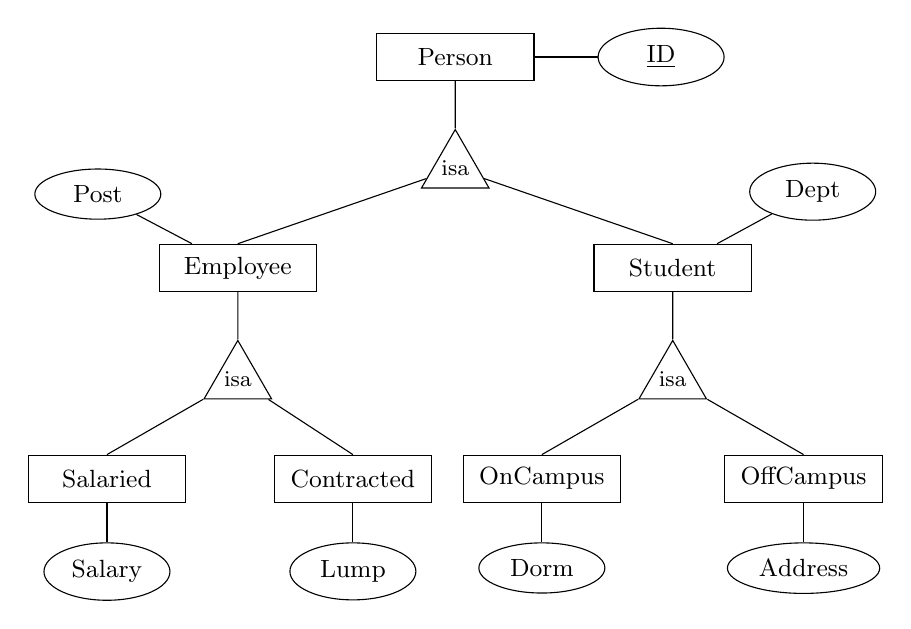
\begin{tikzpicture}[
        % Define styles for ER diagram elements
        entity/.style={rectangle, draw, minimum width=2cm, minimum height=0.6cm, font=\small},
        attribute/.style={ellipse, draw, minimum width=1.6cm, minimum height=0.6cm, font=\small},
        isa/.style={regular polygon, regular polygon sides=3, draw, minimum size=0.6cm, font=\footnotesize, inner sep=0pt}
    ]
        % --------------------------------------------------------
        % LEVEL 0: Root Entity
        % --------------------------------------------------------
        \node[entity] (person) {Person};
        \node[attribute, right=0.8cm of person] (id) {\underline{ID}};
        \draw (person) -- (id);

        % First ISA Hierarchy
        \node[isa, below=0.6cm of person] (isa1) {isa};
        \draw (person) -- (isa1);

        % --------------------------------------------------------
        % LEVEL 1: Sub-entities (Employee & Student)
        % --------------------------------------------------------
        \node[entity, below left=0.7cm and 1.5cm of isa1] (employee) {Employee};
        \node[entity, below right=0.7cm and 1.5cm of isa1] (student) {Student};
        
        \draw (isa1) -- (employee.north);
        \draw (isa1) -- (student.north);

        % Attributes for Level 1
        \node[attribute, above left=0.4cm and 0.2cm of employee] (post) {Post};
        \node[attribute, above right=0.4cm and 0.2cm of student] (dept) {Dept};
        \draw (employee) -- (post);
        \draw (student) -- (dept);

        % --------------------------------------------------------
        % LEVEL 2a: Employee Hierarchy
        % --------------------------------------------------------
        \node[isa, below=0.6cm of employee] (isa2) {isa};
        \draw (employee) -- (isa2);

        \node[entity, below left=0.7cm and 0.4cm of isa2] (salaried) {Salaried};
        \node[entity, below right=0.7cm and 0.2cm of isa2] (contracted) {Contracted};
        
        \draw (isa2) -- (salaried.north);
        \draw (isa2) -- (contracted.north);

        % Attributes for Employee Sub-types
        \node[attribute, below=0.5cm of salaried] (salary) {Salary};
        \node[attribute, below=0.5cm of contracted] (lump) {Lump};
        \draw (salaried) -- (salary);
        \draw (contracted) -- (lump);

        % --------------------------------------------------------
        % LEVEL 2b: Student Hierarchy
        % --------------------------------------------------------
        \node[isa, below=0.6cm of student] (isa3) {isa};
        \draw (student) -- (isa3);

        \node[entity, below left=0.7cm and 0.4cm of isa3] (oncampus) {OnCampus};
        \node[entity, below right=0.7cm and 0.4cm of isa3] (offcampus) {OffCampus};
        
        \draw (isa3) -- (oncampus.north);
        \draw (isa3) -- (offcampus.north);

        % Attributes for Student Sub-types
        \node[attribute, below=0.5cm of oncampus] (dorm) {Dorm};
        \node[attribute, below=0.5cm of offcampus] (address) {Address};
        \draw (oncampus) -- (dorm);
        \draw (offcampus) -- (address);

    \end{tikzpicture}
\end{center}

\mk{15} \yr{CSE 303 | L-3/T-1 | 2012--13}


%% Q4
\item Convert the following E-R diagram into a relational schema:

\medskip
\begin{center}
      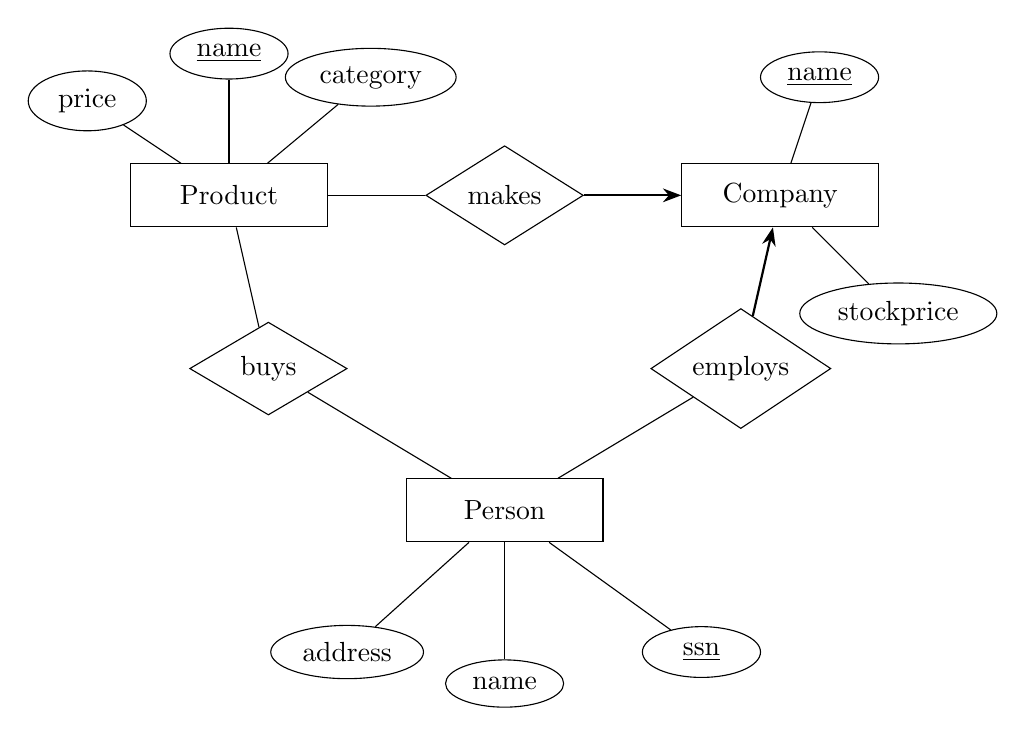
\begin{tikzpicture}[
        >=Stealth, % Arrowhead style
        entity/.style={rectangle, draw, minimum width=2.5cm, minimum height=0.8cm, align=center},
        relationship/.style={diamond, draw, minimum width=2cm, minimum height=1cm, aspect=1.5, align=center},
        attribute/.style={ellipse, draw, minimum width=1.5cm, minimum height=0.6cm, align=center},
        every edge/.style={draw}
    ]

    % ==========================================
    % 1. ENTITIES
    % ==========================================
    \node[entity] (Product) at (0, 0) {Product};
    \node[entity] (Company) at (7, 0) {Company};
    \node[entity] (Person)  at (3.5, -4) {Person};

    % ==========================================
    % 2. RELATIONSHIPS
    % ==========================================
    \node[relationship] (makes)   at (3.5, 0) {makes};
    \node[relationship] (buys)    at (0.5, -2.2) {buys};
    \node[relationship] (employs) at (6.5, -2.2) {employs};

    % ==========================================
    % 3. ATTRIBUTES
    % ==========================================
    
    % Product Attributes
    \node[attribute] (price)    at (-1.8, 1.2) {price};
    \node[attribute] (p_name)   at (0, 1.8) {\underline{name}};
    \node[attribute] (category) at (1.8, 1.5) {category};

    \draw (Product) -- (price);
    \draw (Product) -- (p_name);
    \draw (Product) -- (category);

    % Company Attributes
    \node[attribute] (c_name)     at (7.5, 1.5) {\underline{name}};
    \node[attribute] (stockprice) at (8.5, -1.5) {stockprice};

    \draw (Company) -- (c_name);
    \draw (Company) -- (stockprice);

    % Person Attributes
    \node[attribute] (address)  at (1.5, -5.8) {address};
    \node[attribute] (per_name) at (3.5, -6.2) {name};
    \node[attribute] (ssn)      at (6, -5.8) {\underline{ssn}};

    \draw (Person) -- (address);
    \draw (Person) -- (per_name);
    \draw (Person) -- (ssn);

    % ==========================================
    % 4. RELATIONSHIP CONNECTIONS (LINES & ARROWS)
    % ==========================================
    
    % Product -> makes -> Company
    \draw (Product) -- (makes);
    \draw[->, thick] (makes) -- (Company);

    % Person -> buys -> Product
    \draw (Person) -- (buys);
    \draw (buys) -- (Product);

    % Person -> employs -> Company
    \draw (Person) -- (employs);
    \draw[->, thick] (employs) -- (Company);

    \end{tikzpicture}
\end{center}

\mk{6} \yr{CSE 303 | L-3/T-1 | 2015--16}

%% Q5
\item What are the advantages and disadvantages of storing derived attributes in tables?
\mk{8} \yr{CSE 303 | L-3/T-1 | 2013--14}

%% Q6
\item Discuss with example the difference between strong and weak relationships in the context of relational database modelling. How does security concern arise by the choice of primary key?
\mk{10} \yr{CSE 303 | L-3/T-1 | 2014--15}

%% Q7 — 2016-17 Car rental SQL:99 schema with inheritance
\item A car rental company maintains a database for all vehicles. For all vehicles: vehicle identification number, license number, manufacturer, size (height, width, length) and color. Special data for certain types:
\begin{itemize}[leftmargin=1.5em,itemsep=1pt]
  \item \textbf{Trucks:} load capacity, type
  \item \textbf{Sports car:} power, renter age
  \item \textbf{Bus:} number of passengers, seat-type (array of 40 seats of different types)
\end{itemize}
\begin{enumerate}
  \item Construct an SQL:99 schema definition for this database using appropriate inheritance.
  \item Write constructor functions for the above schema and an insert statement to insert data.
\end{enumerate}
\mk{20} \yr{CSE 303 | L-3/T-1 | 2016--17}

%% Q8 — 2017-18 ISA hierarchy conversion
\item Convert the ISA-hierarchies of the following ER diagram into schemas using three principal conversion strategies.

\medskip
\begin{center}
      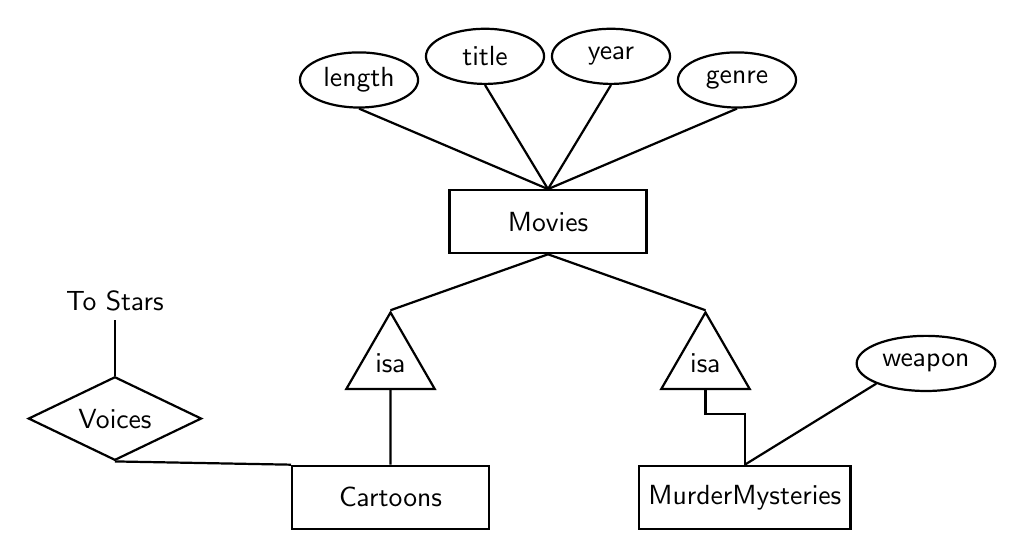
\begin{tikzpicture}[
        thick,
        font=\sffamily,
        % Styles for the ERD components
        entity/.style={
            rectangle, draw, fill=white,
            minimum width=2.5cm, minimum height=0.8cm, 
            align=center
        },
        attribute/.style={
            ellipse, draw, fill=white,
            inner sep=2pt, minimum width=1.5cm, minimum height=0.7cm, 
            align=center
        },
        relationship/.style={
            diamond, draw, fill=white,
            aspect=2, minimum width=2.2cm, minimum height=1cm, 
            align=center
        },
        isa/.style={
            regular polygon, regular polygon sides=3, draw, fill=white,
            inner sep=1pt, minimum size=1cm, align=center
        }
    ]

    % 1. MAIN ENTITY
    \node[entity] (Movies) at (0, 0) {Movies};

    % 2. ATTRIBUTES FOR 'MOVIES'
    \node[attribute] (length) at (-2.4, 1.8) {length};
    \node[attribute] (title)  at (-0.8, 2.1) {title};
    \node[attribute] (year)   at (0.8, 2.1) {year};
    \node[attribute] (genre)  at (2.4, 1.8) {genre};

    % Connect attributes to the top-center of Movies entity
    \draw (Movies.north) -- (length.south);
    \draw (Movies.north) -- (title.south);
    \draw (Movies.north) -- (year.south);
    \draw (Movies.north) -- (genre.south);

    % 3. ISA RELATIONSHIPS (Triangles)
    \node[isa] (isa1) at (-2, -1.8) {isa};
    \node[isa] (isa2) at (2, -1.8) {isa};

    % Connect Movies to the top apex of the ISA triangles
    \draw (Movies.south) -- (isa1.north);
    \draw (Movies.south) -- (isa2.north);

    % 4. SUBCLASSES (Entities)
    \node[entity] (Cartoons) at (-2, -3.5) {Cartoons};
    \node[entity] (MM) at (2.5, -3.5) {MurderMysteries};

    % Connect ISA bases to the subclass entities
    \draw (isa1.south) -- (Cartoons.north);
    \draw (isa2.south) -- ++(0, -0.3) -| (MM.north); % Small adjustment for alignment

    % 5. EXTERNAL RELATIONSHIP FOR 'CARTOONS'
    \node[relationship] (Voices) at (-5.5, -2.5) {Voices};
    \node (ToStars) at (-5.5, -1) {To Stars};
    
    % Connect Cartoons to Voices, and Voices to "To Stars"
    \draw (Cartoons.north west) -- (Voices.south);
    \draw (Voices.north) -- (ToStars.south);

    % 6. ATTRIBUTE FOR 'MURDER MYSTERIES'
    \node[attribute] (weapon) at (4.8, -1.8) {weapon};
    
    % Connect attribute to subclass
    \draw (MM.north) -- (weapon.south west);

    \end{tikzpicture}
\end{center}

\mk{10} \yr{CSE 215 | L-2/T-2 | 2017--18}

%% Q9 — 2018-19 redundancy and incompleteness
\item How can redundancy and incompleteness lead to a bad database design? Explain with appropriate examples.
\mk{10} \yr{CSE 215 | L-2/T-2 | 2018--19}

%% Q10 — 2018-19 production tracking ER to schema
\item Production tracking is important in many manufacturing environments (e.g., the pharmaceuticals
industry, children's toys, etc.). The ER diagram of Figure 3 captures important
information of production tracking. Specifically, the ER diagram captures the relationships
among production lots (or batches), individual production units, and raw materials.

\begin{center}
  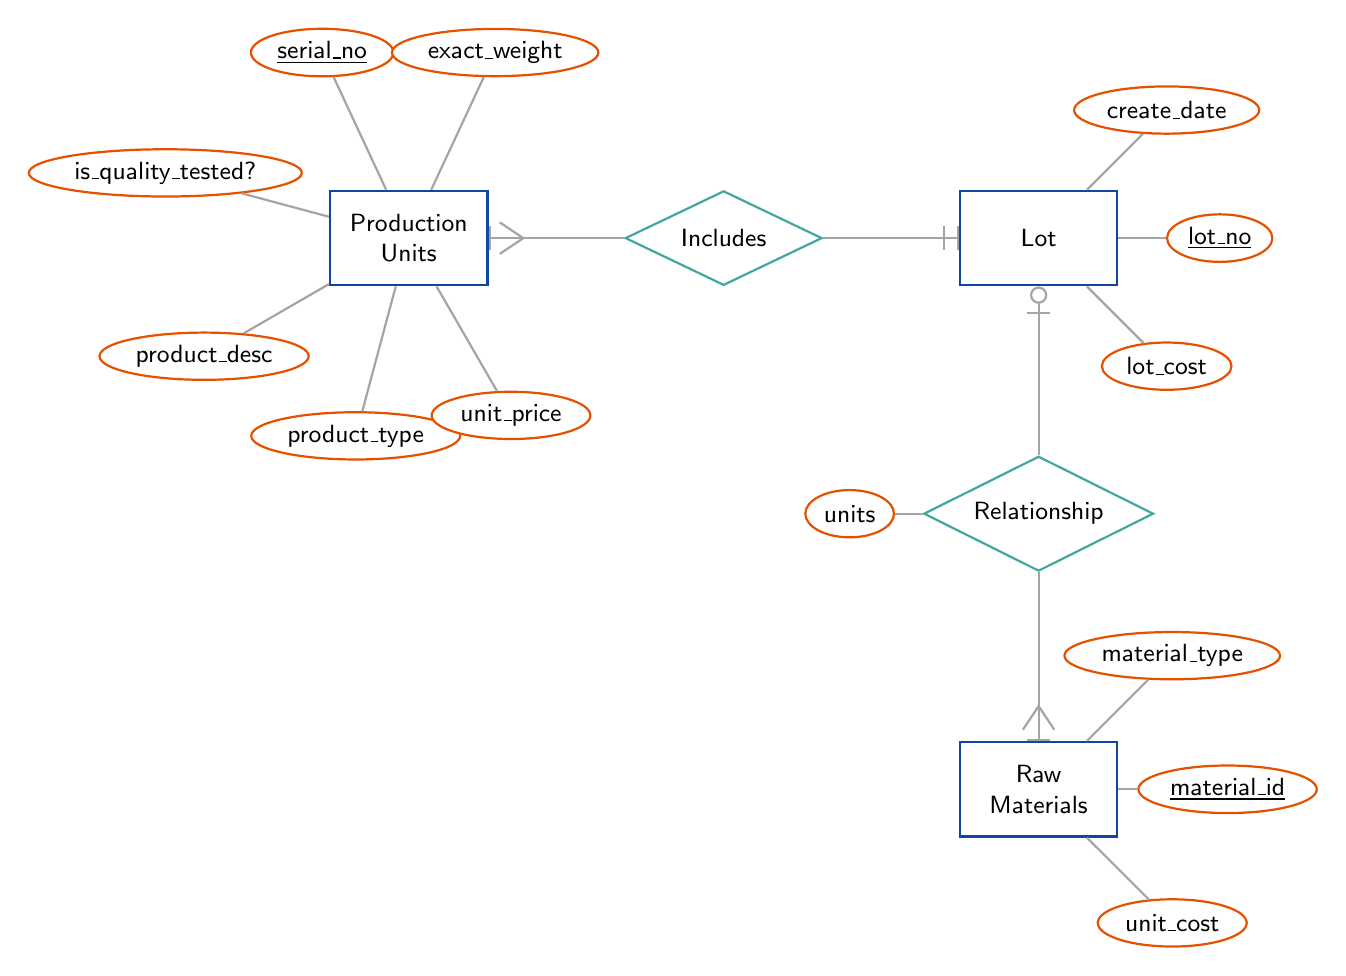
\begin{tikzpicture}[
        >=Stealth,
        font=\sffamily\small,
        % Styles for nodes
        entity/.style={
            rectangle, draw=pblue, thick, fill=white,
            minimum width=2cm, minimum height=1.2cm,
            align=center
        },
        relationship/.style={
            diamond, draw=relborder, thick, fill=white,
            aspect=2, minimum width=2.5cm, minimum height=1.2cm,
            align=center
        },
        attribute/.style={
            ellipse, draw=cE, thick, fill=white,
            inner sep=2pt, minimum height=0.6cm,
            align=center
        },
        % Style for connecting lines
        conn/.style={
            draw=linecol, thick
        },
        % Fixed ERD arrow tips (sep is now a parameter inside the arrow brackets)
        many_mandatory/.style={
            -{Straight Barb[reversed, length=3mm, width=4mm, sep=1mm] |[width=3mm]}
        },
        one_mandatory/.style={
            -{|[width=3mm, sep=1.5mm] |[width=3mm]}
        },
        one_optional/.style={
            -{|[width=3mm, sep=1mm] Circle[open, length=2.2mm]}
        }
    ]

    % 1. MAIN ENTITIES & RELATIONSHIPS
    \node[entity]       (PU)  at (0, 0)     {Production\\Units};
    \node[relationship] (Inc) at (4, 0)     {Includes};
    \node[entity]       (Lot) at (8, 0)     {Lot};
    \node[relationship] (Rel) at (8, -3.5)  {Relationship};
    \node[entity]       (RM)  at (8, -7)    {Raw\\Materials};

    % 2. ERD RELATIONSHIP CONNECTORS
    % Production Units <|--| Includes
    \draw[conn, many_mandatory] (Inc.west) -- (PU.east);
    
    % Includes --|| Lot
    \draw[conn, one_mandatory]  (Inc.east) -- (Lot.west);
    
    % Lot --|o Relationship
    \draw[conn, one_optional]   (Rel.north) -- (Lot.south);
    
    % Relationship --|< Raw Materials
    \draw[conn, many_mandatory] (Rel.south) -- (RM.north);

    % 3. ATTRIBUTES
    
    % Production Units Attributes
    \node[attribute] (PU_serial) at ($(PU) + (115:2.6)$) {\underline{serial\_no}};
    \node[attribute] (PU_weight) at ($(PU) + (65:2.6)$)  {exact\_weight};
    \node[attribute] (PU_qual)   at ($(PU) + (165:3.2)$) {is\_quality\_tested?};
    \node[attribute] (PU_desc)   at ($(PU) + (210:3.0)$) {product\_desc};
    \node[attribute] (PU_type)   at ($(PU) + (255:2.6)$) {product\_type};
    \node[attribute] (PU_price)  at ($(PU) + (300:2.6)$) {unit\_price};
    
    \draw[conn] (PU) -- (PU_serial);
    \draw[conn] (PU) -- (PU_weight);
    \draw[conn] (PU) -- (PU_qual);
    \draw[conn] (PU) -- (PU_desc);
    \draw[conn] (PU) -- (PU_type);
    \draw[conn] (PU) -- (PU_price);

    % Lot Attributes
    \node[attribute] (Lot_date) at ($(Lot) + (45:2.3)$)  {create\_date};
    \node[attribute] (Lot_no)   at ($(Lot) + (0:2.3)$)   {\underline{lot\_no}};
    \node[attribute] (Lot_cost) at ($(Lot) + (-45:2.3)$) {lot\_cost};
    
    \draw[conn] (Lot) -- (Lot_date);
    \draw[conn] (Lot) -- (Lot_no);
    \draw[conn] (Lot) -- (Lot_cost);

    % Relationship Attributes
    \node[attribute] (Rel_units) at ($(Rel) + (180:2.4)$) {units};
    \draw[conn] (Rel) -- (Rel_units);

    % Raw Materials Attributes
    \node[attribute] (RM_type) at ($(RM) + (45:2.4)$)  {material\_type};
    \node[attribute] (RM_id)   at ($(RM) + (0:2.4)$)   {\underline{material\_id}};
    \node[attribute] (RM_cost) at ($(RM) + (-45:2.4)$) {unit\_cost};
    
    \draw[conn] (RM) -- (RM_type);
    \draw[conn] (RM) -- (RM_id);
    \draw[conn] (RM) -- (RM_cost);

    \end{tikzpicture}
\end{center}
\mk{10} \yr{CSE 215 | L-2/T-2 | 2018--19}

%% Q11 — 2019-20 university ER diagram (professors, graduate students, projects, departments)
\item Consider the following information about a university database:
\begin{itemize}[leftmargin=1.5em,itemsep=1pt]
  \item Professors have an SSN, a name, an age, a rank, and a research specialty.
  \item Projects have a project number, a sponsor name, a starting date, an ending date, and a budget.
  \item Graduate students have an SSN, a name, an age, and a degree program (e.g., M.S.\ or Ph.D.).
  \item Each project is managed by one professor (principal investigator) and worked on by one or more professors (co-investigators).
  \item Each project is worked on by one or more graduate students (research assistants); a professor must supervise their work. Graduate students can work on multiple projects with a (potentially different) supervisor for each.
  \item Departments have a department number, name, and main office; a professor (chairman) runs the department.
  \item Professors work in one or more departments with an associated time percentage.
  \item Graduate students have one major department and a more senior graduate student advisor.
  \item Both professors and graduate students have multiple phone numbers and email addresses.
\end{itemize}
\begin{enumerate}
  \item Draw an ER diagram that captures the above information. Indicate all key and cardinality constraints and any assumptions you make.
  \item Convert the above ER diagram into relational schema.
\end{enumerate}
\mk{35} \yr{CSE 215 | L-2/T-2 | 2019--20}

%% Q12 — 2019-20 employee ERD (technical/non-technical ISA) + two relational schemas
\item All employees in an organization are identified by employee id. All employees must have name, address, mobile and email. An employee must be one of the following: technical or non-technical. Technical employees have the trade and year of experience. Non-technical employees have the highest degree and year of experience. Each employee is managed by a manager who is also an employee. Draw the complete ERD for this scenario. Convert the ER diagram into two different possible relational schemas.
\mk{15} \yr{CSE 215 | L-2/T-2 | 2019--20}

%% Q13 — 2019-20 materialized view
\item What do you mean by materialized view? Explain with examples the problems associated with materialized view. What restrictions do most database implementations have to allow updates on materialized views?
\mk{10} \yr{CSE 215 | L-2/T-2 | 2019--20}

\item Reduce the given ERD to the minimum relational schemas (mention schema names and their attributes).

\begin{center}
  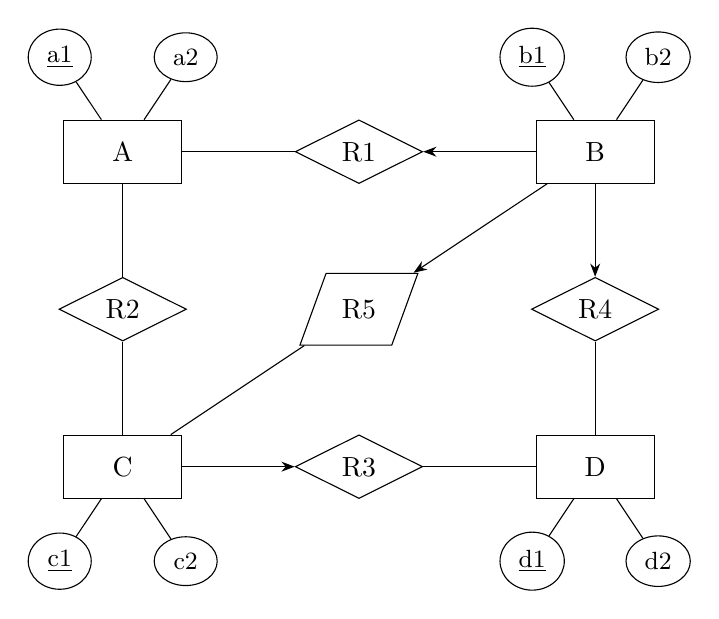
\begin{tikzpicture}[
        >=Stealth, % Sets arrow style
        entity/.style={draw, rectangle, minimum width=1.5cm, minimum height=0.8cm},
        relationship/.style={draw, diamond, aspect=2, minimum width=1.5cm, minimum height=0.8cm},
        attribute/.style={draw, ellipse, minimum width=0.8cm, minimum height=0.5cm, font=\small},
        % R5 is uniquely drawn as a parallelogram in the image
        parallelogram/.style={draw, trapezium, trapezium left angle=70, trapezium right angle=110, minimum width=1.5cm, inner xsep=0pt}
    ]

    % --- Entities ---
    \node[entity] (A) at (0, 0) {A};
    \node[entity] (B) at (6, 0) {B};
    \node[entity] (C) at (0, -4) {C};
    \node[entity] (D) at (6, -4) {D};

    % --- Relationships ---
    \node[relationship] (R1) at (3, 0) {R1};
    \node[relationship] (R2) at (0, -2) {R2};
    \node[relationship] (R3) at (3, -4) {R3};
    \node[relationship] (R4) at (6, -2) {R4};
    \node[parallelogram] (R5) at (3, -2) {R5}; 

    % --- Attributes for Entity A ---
    \node[attribute] (a1) at (-0.8, 1.2) {\underline{a1}};
    \node[attribute] (a2) at (0.8, 1.2) {a2};
    \draw (A) -- (a1);
    \draw (A) -- (a2);

    % --- Attributes for Entity B ---
    \node[attribute] (b1) at (5.2, 1.2) {\underline{b1}};
    \node[attribute] (b2) at (6.8, 1.2) {b2};
    \draw (B) -- (b1);
    \draw (B) -- (b2);

    % --- Attributes for Entity C ---
    \node[attribute] (c1) at (-0.8, -5.2) {\underline{c1}};
    \node[attribute] (c2) at (0.8, -5.2) {c2};
    \draw (C) -- (c1);
    \draw (C) -- (c2);

    % --- Attributes for Entity D ---
    \node[attribute] (d1) at (5.2, -5.2) {\underline{d1}};
    \node[attribute] (d2) at (6.8, -5.2) {d2};
    \draw (D) -- (d1);
    \draw (D) -- (d2);

    % --- Edges between Entities and Relationships ---
    
    % R1: A and B
    \draw (A) -- (R1);
    \draw[<-] (R1) -- (B); % Arrow points to R1 from B

    % R2: A and C
    \draw (A) -- (R2);
    \draw (C) -- (R2);

    % R3: C and D
    \draw[<-] (R3) -- (C); % Arrow points to R3 from C
    \draw (D) -- (R3);

    % R4: B and D
    \draw[<-] (R4) -- (B); % Arrow points to R4 from B
    \draw (D) -- (R4);

    % R5: B and C
    \draw[<-] (R5) -- (B); % Arrow points to R5 from B
    \draw (C) -- (R5);

    \end{tikzpicture}
\end{center}

\mk{10} \yr{CSE 215 | L-2/T-2 | 2019--20}



%% Q14 — 2020-21 E/R diagram for ER diagram truth statements (Enroll, Teacher, Student, Course)
\item For the given E-R diagram with entities \textbf{Teacher}, \textbf{Student}, \textbf{Course}, and weak entity \textbf{Enroll}, determine which of the following statements hold:

\begin{center}
  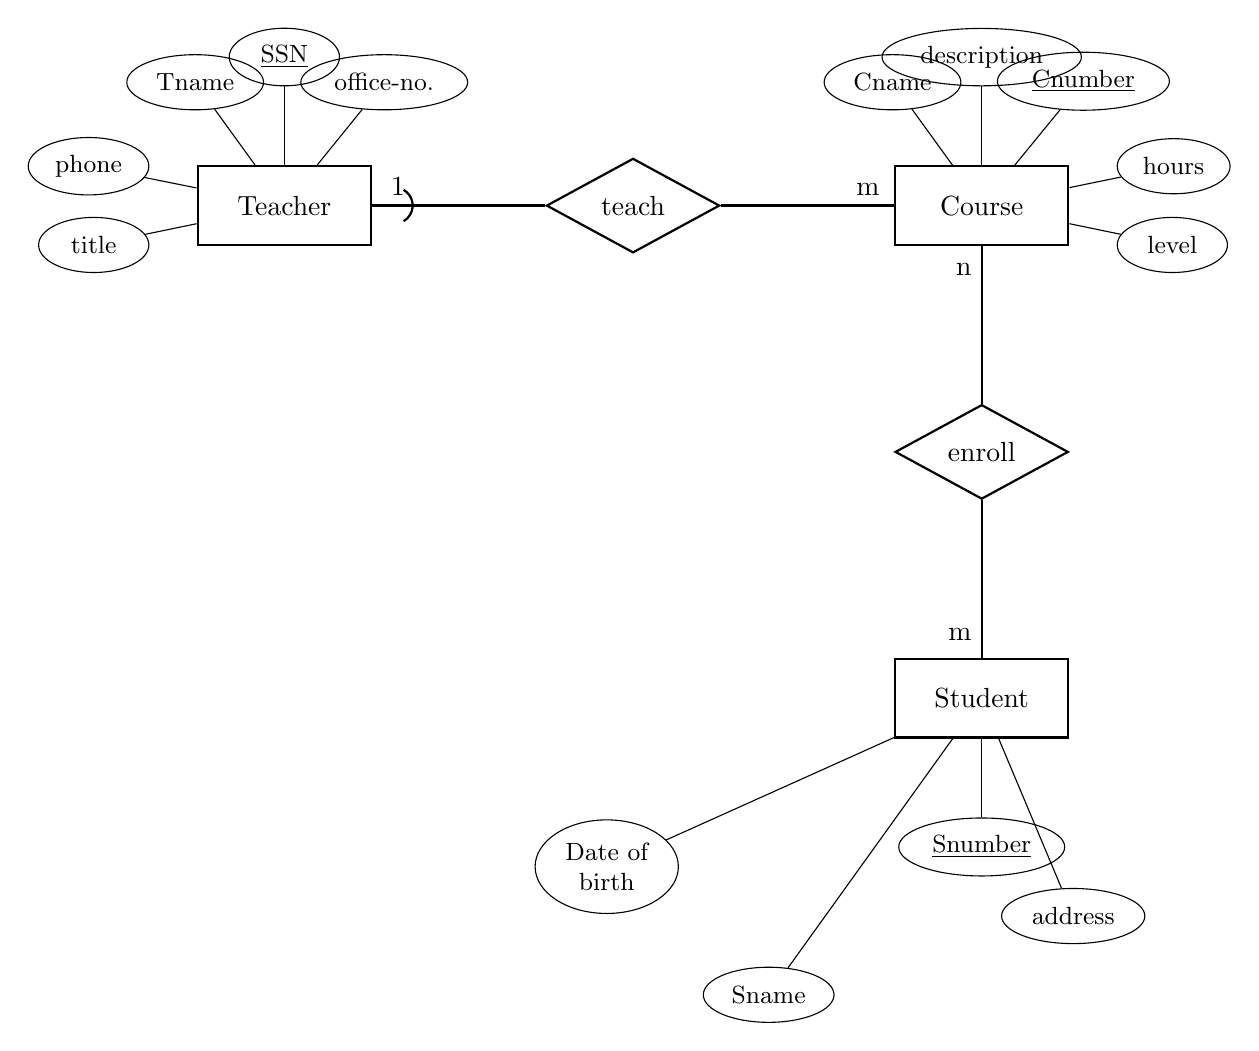
\begin{tikzpicture}[
        % Define styles for E/R diagram components
        entity/.style={draw, thick, rectangle, minimum width=2.2cm, minimum height=1cm, align=center},
        relationship/.style={draw, thick, diamond, aspect=2, minimum width=2.2cm, minimum height=1.2cm, align=center},
        attribute/.style={draw, thin, ellipse, minimum width=1.4cm, minimum height=0.7cm, align=center, font=\small}
    ]
    
    % --- ENTITIES & RELATIONSHIPS ---
    % Teacher Entity and its attributes
    \node[entity] (teacher) {Teacher};
    
    % teach Relationship
    \node[relationship, right=2.2cm of teacher] (teach) {teach};
    
    % Course Entity
    \node[entity, right=2.2cm of teach] (course) {Course};
    
    % enroll Relationship
    \node[relationship, below=2cm of course] (enroll) {enroll};
    
    % Student Entity
    \node[entity, below=2cm of enroll] (student) {Student};
    
    
    % --- ATTRIBUTES ---
    % Teacher Attributes
    \node[attribute, left=0.6cm of teacher, yshift=-0.5cm] (title) {title};
    \node[attribute, left=0.6cm of teacher, yshift=0.5cm] (phone) {phone};
    \node[attribute, above left=0.8cm and -0.6cm of teacher] (tname) {Tname};
    \node[attribute, above=1cm of teacher] (ssn) {\underline{SSN}};
    \node[attribute, above right=0.8cm and -0.6cm of teacher] (office) {office-no.};
    
    % Course Attributes
    \node[attribute, above left=0.8cm and -0.6cm of course] (cname) {Cname};
    \node[attribute, above=1cm of course] (desc) {description};
    \node[attribute, above right=0.8cm and -0.6cm of course] (cnumber) {\underline{Cnumber}};
    \node[attribute, right=0.6cm of course, yshift=0.5cm] (hours) {hours};
    \node[attribute, right=0.6cm of course, yshift=-0.5cm] (level) {level};
    
    % Student Attributes
    \node[attribute, below left=1.2cm and 3cm of student] (dob) {Date of\\birth};
    \node[attribute, below left=3cm and 1cm of student] (sname) {Sname};
    \node[attribute, below=1cm of student] (snumber) {\underline{Snumber}};
    \node[attribute, below right=2cm and -0.6cm of student] (address) {address};
    
    
    % --- CONNECTIONS & CARDINALITY ---
    % Connect Teacher to its attributes
    \draw (teacher) -- (title);
    \draw (teacher) -- (phone);
    \draw (teacher) -- (tname);
    \draw (teacher) -- (ssn);
    \draw (teacher) -- (office);
    
    % Connect Course to its attributes
    \draw (course) -- (cname);
    \draw (course) -- (desc);
    \draw (course) -- (cnumber);
    \draw (course) -- (hours);
    \draw (course) -- (level);
    
    % Connect Student to its attributes
    \draw (student) -- (dob);
    \draw (student) -- (sname);
    \draw (student) -- (snumber);
    \draw (student) -- (address);
    
    % Connect Entities via Relationships with Cardinality Labels
    % Teacher to teach (with optional arc indicator simulation)
    \draw[thick] (teacher) -- node[above, pos=0.15] {1} (teach);
    % Small arc indicator next to Teacher
    \draw[thick] ([xshift=4mm, yshift=2mm]teacher.east) arc (60:-60:2.3mm);
    
    \draw[thick] (teach) -- node[above, pos=0.85] {m} (course);
    
    % Course to Student via enroll
    \draw[thick] (course) -- node[left, pos=0.15] {n} (enroll);
    \draw[thick] (enroll) -- node[left, pos=0.85] {m} (student);
    
    \end{tikzpicture}
\end{center}

\begin{enumerate}
  \item Enroll is a strong entity set.
  \item All teachers must teach courses.
  \item All students must enroll in courses.
  \item All courses must be enrolled by students.
  \item All courses must be taught by teachers.
  \item Each course is taught by only one teacher.
  \item Each course is enrolled by only one student.
  \item Each teacher may teach many courses.
  \item Each student can enroll in many courses.
  \item Teacher is a relationship set.
\end{enumerate}
\mk{10} \yr{CSE 215 | L-2/T-2 | 2020--21}

%% Q15 — 2020-21 blog platform E/R and SQL schema
\item You are running a startup company allowing users to post blogs and comment on other users' blogs.
\begin{enumerate}
  \item Design the E/R diagram for your company's data. Store information about users, bloggers, and blogs. Every user has a user ID and a name. Every blog has a blog ID, text content, and one author (a blogger). Every blogger is a user with a rating attribute. Users may comment on blogs. Every comment has optional text content and/or an optional rating.
  \item Write a sequence of SQL queries that create the tables for this E/R diagram; \texttt{uid}, \texttt{bid}, and \texttt{rating} are integers, all other attributes are text. Include key, foreign key, and not null declarations.
\end{enumerate}
\mk{20} \yr{CSE 215 | L-2/T-2 | 2020--21}

%% Q16 — 2020-21 multi-way relationship (Actor, Film, Studio)
\item Consider a multi-way relationship between \textbf{Actor}, \textbf{Film} and \textbf{Studio}.
\begin{enumerate}
  \item There is an arrow pointing to entity set Studios. What is its interpretation?
  \item There are no arrows pointing to entity sets Actor or Film. What are their interpretations?
\end{enumerate}
\begin{center}
  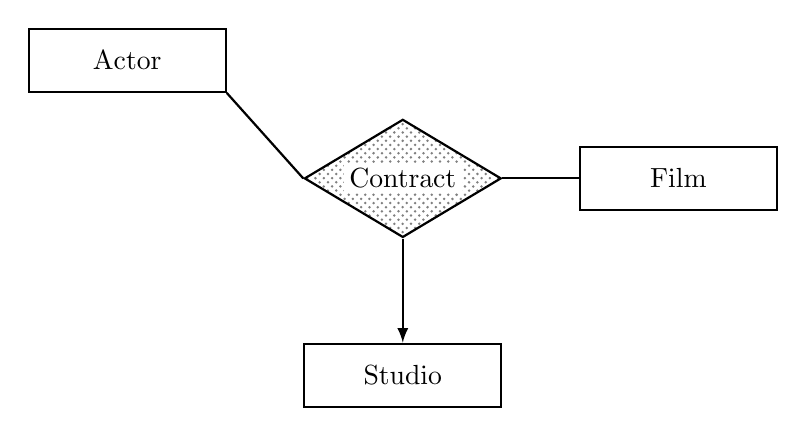
\begin{tikzpicture}[
        thick,
        % Define styles for the boxes and diamond
        entity/.style={draw, rectangle, minimum width=2.5cm, minimum height=0.8cm, align=center},
        relationship/.style={draw, diamond, aspect=1.5, minimum width=2.5cm, minimum height=1.5cm, align=center, pattern=crosshatch dots, pattern color=gray}
    ]
    
    % Draw the central relationship diamond
    \node[relationship] (contract) at (0,0) {};
    % Place the text over a white background so it is legible against the pattern
    \node at (contract) [fill=white, inner sep=2pt] {Contract};
    
    % Draw the entity nodes
    \node[entity] (actor) at (-3.5, 1.5) {Actor};
    \node[entity] (film) at (3.5, 0) {Film};
    \node[entity] (studio) at (0, -2.5) {Studio};
    
    % Draw the connecting lines
    \draw (actor.south east) -- (contract.west);
    \draw (contract.east) -- (film.west);
    \draw[-latex] (contract.south) -- (studio.north);
    
    \end{tikzpicture}
\end{center}

\mk{5} \yr{CSE 215 | L-2/T-2 | 2020--21}

%% Q17 — 2021-22 BPL database ER diagram
\item Suppose you are given the following requirements for a simple database for the Bangladesh Premier League (BPL) in a season:
\begin{itemize}[leftmargin=1.5em,itemsep=1pt]
  \item The BPL has many teams; each team has a name, a city, a coach, a captain, and a set of players.
  \item Each player belongs to only one team; a player may not be hired by any team.
  \item Each player has a name, a fielding position (such as slip, mid-wicket, long on, long off etc), a ranking, and a set of injury records.
  \item A team captain is also a player.
  \item Injury records must have an id, period (start and end), and a short description.
  \item A game is played between two teams (host\_team and guest\_team) with a date (such as May 11th, 2023) and scores (winning and losing team scores such as 143/10 and 148/6).
\end{itemize}
Construct a clean and concise E/R diagram for the BPL database. List your assumptions and clearly indicate cardinality mappings and any role indicators.
\mk{10} \yr{CSE 215 | L-2/T-2 | 2021--22}

%% Q18 — 2021-22 employee organization ERD with subclasses + conversion
\item Consider the following descriptions of an organization having many EMPLOYEES. \hfill \textbf{(10+10=20)}

\begin{enumerate}[label=(\roman*)]
    \item An EMPLOYEE has a name, nid number, data of birth, and address.
    \item Based on the EMPLOYEE's Job, EMPLOYEE may be further grouped into:\\
    SECRETARY, ENGINEER, TECHNICIAN, and MANAGER
    \item Based on the EMPLOYEE's method of pay, EMPLOYEE may also be grouped into:\\
    SALARIED\_EMPLOYEE, and HOURLY\_EMPLOYEE
    \item A salaried employee who is also an engineer belongs to the two subclasses:\\
    ENGINEER, and SALARIED\_EMPLOYEE
    \item A salaried employee who is also an engineering manager belongs to the three subclasses:\\
    MANAGER, ENGINEER, and SALARIED\_EMPLOYEE.
    \item We want to record typing speed of each SECRETARY.
    \item Each technician has a technical grade ( a number) which depends on his skill level
    \item Each Engineer has a type (ME, CSE, EEE, etc \dots)
    \item Each MANAGER manages at least one project, each project has a project id, title, and a project value.
    \item Each HOURLY\_EMPLOYEE is a member of some TRADE\_UNION which has a name and member count.
\end{enumerate}

\begin{itemize}
    \item Construct an E/R diagram with the above description; clearly indicate the cardinality mappings as well as any role indicators in your E/R diagram.
    \item Convert the E/R diagram into a set of relational database schema. You should avoid keeping null values in attributes.
\end{itemize}
\mk{20} \yr{CSE 215 | L-2/T-2 | 2021--22}

%% Q19 — 2021-22 ISA subclass (Courses -> Lab Courses, Depts) conversion
\item Convert the E/R diagram of Figure below into a relational database schema.

\begin{center}
  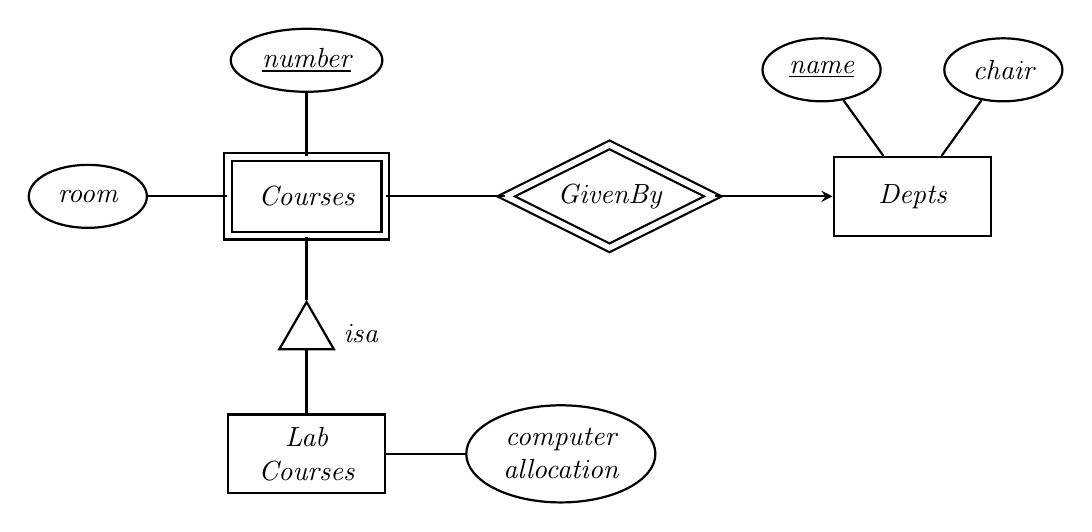
\begin{tikzpicture}[
        >=stealth, % Arrow style
        % Define node styles
        entity/.style={draw, thick, rectangle, minimum width=2cm, minimum height=1cm, align=center, font=\itshape},
        weak entity/.style={entity, double, double distance=2pt},
        relationship/.style={draw, thick, diamond, aspect=2, minimum width=2.5cm, minimum height=1.2cm, align=center, font=\itshape},
        weak relationship/.style={relationship, double, double distance=2pt},
        attribute/.style={draw, thick, ellipse, minimum width=1.5cm, minimum height=0.8cm, align=center, font=\itshape},
        isa/.style={draw, thick, regular polygon, regular polygon sides=3, minimum size=0.8cm, inner sep=0pt}
    ]
    
    % --- Entities & Relationships ---
    
    % Center Weak Entity
    \node[weak entity] (Courses) {Courses};
    
    % Identifying Relationship (Double Diamond)
    \node[weak relationship, right=1.5cm of Courses] (GivenBy) {GivenBy};
    
    % Regular Entity
    \node[entity, right=1.5cm of GivenBy] (Depts) {Depts};
    
    % ISA Hierarchy (Triangle)
    \node[isa, below=0.8cm of Courses] (isa_triangle) {};
    \node[right=0.1cm of isa_triangle, font=\itshape] {isa}; % Label next to triangle
    
    % Subclass Entity
    \node[entity, below=0.8cm of isa_triangle] (LabCourses) {Lab\\Courses};
    
    
    % --- Attributes ---
    
    % Courses Attributes
    \node[attribute, above=0.8cm of Courses] (number) {\underline{number}};
    \node[attribute, left=1cm of Courses] (room) {room};
    
    % Depts Attributes
    \node[attribute, above left=0.8cm and -0.4cm of Depts] (name) {\underline{name}};
    \node[attribute, above right=0.8cm and -0.4cm of Depts] (chair) {chair};
    
    % Lab Courses Attributes
    \node[attribute, right=1cm of LabCourses] (comp) {computer\\allocation};
    
    
    % --- Connecting Lines ---
    
    % Courses connections
    \draw[thick] (Courses) -- (number);
    \draw[thick] (Courses) -- (room);
    \draw[thick] (Courses) -- (GivenBy);
    
    % GivenBy to Depts (Many-to-One Arrow)
    \draw[thick, ->] (GivenBy) -- (Depts); 
    
    % Depts connections
    \draw[thick] (Depts) -- (name);
    \draw[thick] (Depts) -- (chair);
    
    % ISA connections
    \draw[thick] (Courses) -- (isa_triangle.north);
    \draw[thick] (isa_triangle.south) -- (LabCourses);
    
    % Lab Courses connections
    \draw[thick] (LabCourses) -- (comp);
    
    \end{tikzpicture}
\end{center}


\mk{5} \yr{CSE 215 | L-2/T-2 | 2021--22}

%% Q20 — 2022-23 YouTube ERD (4 parts: user mgmt, video hosting, commenting, subscription)
\item YouTube is a very popular platform for hosting videos. People create channels and
upload videos on that. Sometimes the creators can batch up the videos into playlists.
Videos can be free to view or behind paywall which requires subscription to YouTube.
Premium. A free video can be watched with or without signing into YouTube. However,
only signed-in users' views are considered when counting the number of viewers for a
video. A signed-in account may or may not have corresponding channels. Each video has
a comment section where a signed-in user can comment; and comment to other people’s
comments. Also, videos contain some tags (given by the uploader or YouTube itself) that
help to filter videos. Signed-in users can subscribe to other channels. Now, for each of the
mentioned features below, design the corresponding portion of ERD for YouTube only.
Add attributes as you see fit and mark primary keys.
\begin{enumerate}
  \item \textbf{User management:} Users should be able to create accounts, create channels on top of
the accounts (one¢ user can create at most one channel), and subscribe to different
channels.
  \item \textbf{Video hosting:} Creators should be able to upload videos with different tags, and
create playlists by batching up multiple videos. Users should be able to view the videos,
find them in their history when needed and, also, check the number of viewers to the
videos.
  \item \textbf{Commenting:} Users should be able to comment on any video any number of times,
They should also be able to comment on other peoples comments.
  \item \textbf{Subscription system:} Creators should be able to mark some videos as premium (i.e.,
only subscribed users can view). Users should be able to buy subscriptions up to some
end date.
%% Q21 — 2022-23 YouTube ERD to relational schemas
\item Implement relational schemas for each ERD you designed in this question.
\mk{15} \yr{CSE 215 | L-2/T-1 | 2022--23}
\end{enumerate}
\mk{20} \yr{CSE 215 | L-2/T-1 | 2022--23}



%% Q22 — 2022-23 non-binary relationship + issues
\item Give an example of a Non-Binary Relationship. What issues arise for Non-Binary Relationships?
\mk{5} \yr{CSE 215 | L-2/T-1 | 2022--23}

%% Q23 — 2023-24 library ER diagram
\item A library keeps records of current loans of books to borrowers. Each borrower is identified by a borrower number; each copy of a book by an accession number. The library may hold more than one copy of any given book. Borrower name and address are stored for communications. Book information includes: title, author name(s), publisher name, publication date, ISBN, purchase price, classification (reference or fiction), and number of pages. A book may be written by multiple authors but published by a single publisher. The library uses unique in-house codes for authors and publishers. A book may cover multiple subjects; borrowers can use an online catalogue to select texts by subject, title, or author. There are restrictions on the number of books a borrower may have on loan and the loan period, depending on borrower classification (junior, adult, or organization). When a book is borrowed, the return date is automatically recorded. Other borrowers may reserve books currently on loan; the reservation date is recorded. A borrower status flag is maintained --- borrowers who hold overdue books or have reached their loan limit are flagged to prevent further borrowings.
\begin{enumerate}
  \item Draw an Entity-Relationship (ER) diagram to represent the library data requirements described above.
  \item Identify two attributes in the above scenario which can be derived using business rules. Write the schema description to store these business rules.
\end{enumerate}
\mk{26} \yr{CSE 215 | L-2/T-1 | 2023--24}

%% Q24 — 2023-24 view vs materialized view + disjoint specialization diagram
\item What is the difference between a view and a materialized view? Draw an example diagram of a disjoint specialization.
\mk{10} \yr{CSE 215 | L-2/T-1 | 2023--24}

%% Q25 — 2024-25 ternary to binary relationship conversion procedure
\item Write the general procedure to convert a ternary relationship to binary relationships.
\mk{8} \yr{CSE 215 | L-2/T-1 | 2024--25}

%% Q26 — 2024-25 total vs partial participation using ER diagram example
\item Explain the concept of total and partial participation of entities in a relationship set using an example ER diagram.
\mk{10} \yr{CSE 215 | L-2/T-1 | 2024--25}

%% Q27 — 2024-25 composite and multivalued attributes in ER-to-relational conversion
\item How are composite attributes and multivalued attributes handled when an ER model is transformed into a relational database schema? Explain with examples.
\mk{10} \yr{CSE 215 | L-2/T-1 | 2024--25}

\end{enumerate}


%% ══════════════════════════════════════════════════════════════════════
%%  PART II — QUERY LANGUAGES
%% ══════════════════════════════════════════════════════════════════════
\secdivider{Part II}{Query Languages}{cB}{cB}

%% ── S3: Query Languages ───────────────────────────────────────────────
\section{S3 --- Query Languages}
\label{sec:S3}
\markboth{S3 --- Query Languages}{}

%%──────────────────────────────────────────────────────────────────────
\subtopic{cB}{SQL}
\label{sub:s3-sql}

\begin{enumerate}

%% Q1
\item Consider the following schema:
\begin{center}
\begin{tabular}{l}
\texttt{Product(\underline{pid}, name, price, category, year, maker\_cid)}\\
\texttt{Purchase(\underline{buyer\_ssn}, \underline{seller\_ssn}, store, pid)}\\
\texttt{Company(\underline{cid}, name, stock\_price, country)}\\
\texttt{Person(\underline{ssn}, name, phone\_number, city)}
\end{tabular}
\end{center}
\textit{Note:} In \texttt{Purchase}: \texttt{buyer\_ssn}, \texttt{seller\_ssn} are foreign keys in \texttt{Person}, \texttt{pid} is foreign key in \texttt{Product}; in \texttt{Product} \texttt{maker\_cid} is a foreign key in \texttt{Company}.

Write SQL statements to answer the following queries:
\begin{enumerate}
  \item Find names of people buying telephony products.
  \item Find products (and their manufacturers) that are more expensive than all products made by the same manufacturer before 1972.
  \item Find names of people who bought Bangladeshi products and did not buy Indian products.
  \item Find names of products (and their manufacturers) whose prices are less than the average product price of that company.
\end{enumerate}
\mk{20} \yr{CSE 215 | L-3/T-1 | 2010--11}

%% Q2
\item Consider the following relations:
\begin{center}
\begin{tabular}{l}
\texttt{Emp(\underline{eno}, ename, title, city)}\\
\texttt{Proj(\underline{pno}, pname, budget, city)}\\
\texttt{Works(\underline{eno}, \underline{pno}, resp, dur)}\\
\texttt{Pay(\underline{title}, salary)}
\end{tabular}
\end{center}
where \texttt{Emp.title} is a foreign key to \texttt{Pay.title}, \texttt{Works.eno} is a foreign key to \texttt{Emp.eno} and \texttt{Works.pno} is a foreign key to \texttt{Proj.pno}.

Write SQL statements to answer the following queries:
\begin{enumerate}
  \item For each city, how many projects are located in that city and what is the total budget over all projects in the city?
  \item For each project, what fraction of the budget is spent (in total) on salaries for the people working on that project? Sort your answer by the value of the budget.
  \item Remove the work assignment of all persons to any projects for which more than 2 persons share the same responsibility.
  \item List all projects located in Toronto city and include for each one the number of persons working on the project.
  \item Find the names of projects whose budgets are greater than all projects located in Waterloo city.
\end{enumerate}
\mk{25} \yr{CSE 303 | L-3/T-1 | 2011--12}

%% Q3
\item A database schema consists of four relations:
\begin{center}
\begin{tabular}{l}
\texttt{Product(maker, model, type)}\\
\texttt{PC(model, speed, ram, hd, price)}\\
\texttt{Laptop(model, speed, ram, hd, screen, price)}\\
\texttt{Printer(model, color, type, price)}
\end{tabular}
\end{center}

\begin{enumerate}
\item  Delete all laptops made by a manufacturer that does not make printers.
\mk{5} \yr{CSE 303 | L-3/T-1 | 2011--12}

%% Q4
\item Assume that manufacturer A bought manufacturer B. Change all products made by B so that they are now made by A.
\mk{5} \yr{CSE 303 | L-3/T-1 | 2011--12}
\end{enumerate}
%% Q5
\item What are the three types of relations in SQL?
\mk{5} \yr{CSE 303 | L-3/T-1 | 2012--13}

%% Q6 — 2015-16 PC/Laptop/Printer schema
\item Consider the following relational database schema:
\begin{center}
\begin{tabular}{l}
\texttt{Product(\underline{maker}, model, type)}\\
\texttt{PC(\underline{model}, speed, ram, hd, price)}\\
\texttt{Laptop(\underline{model}, speed, ram, hd, screen, price)}\\
\texttt{Printer(\underline{model}, color, type, price)}
\end{tabular}
\end{center}
The Product relation gives the manufacturer, model number and type (PC, laptop, or
printer) of various products. We assume for convenience that model numbers are
unique over all manufacturers and product types; that assumption is not realistic, and a
real database would include a code for the manufacturer as part of the model number.
The PC relation gives for each model number that is a PC the speed (of the processor,
in gigahertz), the amount of RAM (in megabytes), the size of the hard disk (in
gigabytes), and the price. The Laptop relation is similar, except that the screen size (in
inches) is also included. The Printer relation records for each printer model whether
the printer produces color output ('T', if so; 'F' otherwise), the process type (laser or
ink-jet, typically), and the price.
Write the following SQL queries:
\begin{enumerate}
  \item Find those manufacturers that sell Laptops, but not PCs or Printers.
  \item Find those hard disk sizes that occur in two or more PCs.
  \item Find those pairs of PC models that have both the same speed and RAM. A pair should be listed only once.
  \item Find the manufacturers of PCs with at least three different speeds.
  \item Find the makers who produce only one type of product.
  \item Find the maker(s) of the cheapest color printer(s).
  \item Find the PC model with maximum processing speed without using any aggregate function.
\end{enumerate}
\mk{28} \yr{CSE 303 | L-3/T-1 | 2015--16}

%% Q7 — 2015-16 SQL set operations
\item Consider three tables $T1$, $T2$ and $T3$, each with a single integer column:

\medskip
\begin{center}
\begin{tabular}{lll}
\toprule
\textbf{T1} & \textbf{T2} & \textbf{T3}\\
\midrule
1,2,2,2,3,4,4 & 2,3,4,4,4,5 & 2,2,3,3,4,4,5,5\\
\bottomrule
\end{tabular}
\end{center}

Show the result of the following SQL queries:
\begin{enumerate}
  \item \texttt{SELECT * FROM T1 UNION SELECT * FROM T2}
  \item \texttt{SELECT * FROM T1 MINUS SELECT * FROM T3}
  \item \texttt{(SELECT * FROM T1 UNION ALL SELECT * FROM T2) INTERSECT ALL (SELECT * FROM T3)}
\end{enumerate}
\mk{7} \yr{CSE 303 | L-3/T-1 | 2015--16}

%% Q8 — 2015-16 University DB constraints
\item Consider the following schema:
\begin{center}
\begin{tabular}{l}
\texttt{Department(\underline{name}, headID, yearOfEstablishment)}\\
\texttt{Employee(\underline{id}, name, address, designation, salary, gender)}
\end{tabular}
\end{center}
\begin{enumerate}
  \item Enforce the rule ``Departmental head must be an employee of the university'' --- show two ways: one using a \texttt{CHECK} constraint and one without any check constraint.
  \item Write a \texttt{CHECK} constraint to make sure that no two departments have the same person as Head.
  \item Write an assertion to check: if the Head of the Department's gender is male then his name must not begin with `Ms'.
  \item Write an assertion to check: the CSE Departmental head's salary must not be less than 1,50,000 Taka.
\end{enumerate}
\mk{16} \yr{CSE 303 | L-3/T-1 | 2015--16}

%% Q9 — 2015-16 DDL constraint replacement
\item Answer the following:
\begin{enumerate}
  \item Replace the \texttt{NOT NULL} constraint using a \texttt{CHECK} constraint:\\
  \begin{lstlisting}
  CREATE TABLE MyTable (
      ....
     gender CHAR(1) NOT NULL,
      ....
  );
    \end{lstlisting}
  \item Replace the \texttt{UNIQUE} constraint using a \texttt{CHECK} constraint:\\ 
  \begin{lstlisting}
    CREATE TABLE MyTable (
      .....
      headID INT UNIQUE
      .....
    );
  \end{lstlisting} 
  \item What are the three different policies for \texttt{UPDATE} and \texttt{DELETE} for maintaining referential integrity? Which is more suitable for \texttt{UPDATE} and which for \texttt{DELETE}? Why?
  \item Show the DDL to create a copy of a table $R$ including the schema. What is the DDL if we just want to copy the schema and not the tuples?
\end{enumerate}
\mk{19} \yr{CSE 303 | L-3/T-1 | 2015--16}

%% Q10 — 2014-15 Flights/Aircraft schema
\item Consider the following schema:
\begin{center}
\begin{tabular}{l}
\texttt{Flights(flno: integer, from: string, to: string, distance: interger, departs: integer, arrives: time, price: real)}\\
\texttt{Aircraft(aid: integer, aname: string, cruisingrange: integer)}\\
\texttt{Certified(eid: integer, aid: integer)}\\
\texttt{Employees(eid: integer, ename: string, salary: integer)}
\end{tabular}
\end{center}
Write SQL to implement the following queries:
\begin{enumerate}
  \item Find the names of aircraft such that all pilots certified to operate them have salaries more than \$80,000.
  \item For each pilot certified for more than three aircraft, find the eid and the maximum cruising range of the aircraft for which she or he is certified.
  \item Find the names of pilots whose salary is less than the price of the cheapest route from `Los Angeles' to `Honolulu'.
  \item Find the aids of all aircraft that can be used on routes from `Los Angeles' to `Chicago'.
  \item Identify the routes that can be piloted by every pilot who makes more than \$100,000.
\end{enumerate}
\mk{25} \yr{CSE 303 | L-3/T-1 | 2014--15}

%% Q11 — 2014-15 Roles and privileges
\item Why are roles used for assigning privileges to users? Create three users $U_1$, $U_2$ and $U_3$ and assign \texttt{INSERT} and \texttt{UPDATE} privileges to them on tables $T1$ and $T2$ respectively. Do this by assigning the users a role of ``Admin''. Then transfer these privileges to another role named ``SuperAdmin''. Finally, revoke \texttt{UPDATE} privilege from ``Admin''.
\mk{13} \yr{CSE 303 | L-3/T-1 | 2014--15}

%% Q12 — 2013-14 Patient schema
\item Consider the following schema:
\begin{center}
\begin{tabular}{l}
\texttt{Patient(\underline{ID}, FIRSTNAME, SURNAME, ADMISSION\_DATE, DR\_ID, ward\_no)}\\
\texttt{AILMENT(\underline{AILMENTID}, NAME, PATIENTID)}\\
\texttt{Ward(\underline{ward\_no}, ward\_name)}\\
\texttt{Doctor(\underline{ID}, SURNAME, FIRSTNAME, no\_of\_patient, AILMENTID)}
\end{tabular}
\end{center}
Write SQL to implement the following queries:
\begin{enumerate}
  \item List the surnames of all patients of `Dr.\ Jones'.
  \item List all the doctors who specialise in the ailment suffered by the patient whose surname is `Thomas'.
  \item List the ward number and ward name of the ward(s) which have the most patients.
  \item Provide a list of all patients who have not suffered any ailment.
  \item Show the Doctor's name who has the third highest \texttt{no\_of\_patient}.
\end{enumerate}
\mk{25} \yr{CSE 303 | L-3/T-1 | 2013--14}

%% Q13 — 2013-14 Users and roles
\item Create three users $U_1$, $U_2$ and $U_3$ and assign them \texttt{SELECT} and \texttt{DELETE} privileges respectively on $T1$ and $T2$ tables. Do this by assigning the users a role of ``Admin''. Then transfer these privileges to another role named ``SuperAdmin''.
\mk{8} \yr{CSE 303 | L-3/T-1 | 2013--14}

%% Q14 — 2013-14 Self-referencing constraint
\item How do you insert a tuple without causing a constraint violation in the following table?\\
\texttt{Person(\underline{id}, name, father)} where foreign key \texttt{father} references \texttt{Person}.
\mk{9} \yr{CSE 303 | L-3/T-1 | 2013--14}

%% Q15 — 2016-17 CSE course database
\item Given the relation schema of CSE department course database:
\begin{center}
\begin{tabular}{l}
\texttt{course(\underline{course\_number}, title, credit\_hour, level, term, pre\_req\_course\_number)}\\
\texttt{takes(\underline{course\_number}, \underline{student\_id})}\\
\texttt{student(\underline{student\_id}, name, CGPA)}
\end{tabular}
\end{center}
Write SQL statements to:
\begin{enumerate}
  \item Find the list of only those students who have taken all the courses of level 3 and term 1.
  \item Find the list of courses that are not taken by any student.
  \item Find the student id and the number of courses taken for those students with CGPA higher than 3.5.
\end{enumerate}
\mk{15} \yr{CSE 303 | L-3/T-1 | 2016--17}

%% Q16 — 2016-17 Employee database DDL with constraints
\item Given the employee database:
\begin{center}
\begin{tabular}{l}
\texttt{Employee(\underline{employee\_name}, house\_number, street, city)}\\
\texttt{Works(\underline{employee\_name}, \underline{company\_name}, salary)}\\
\texttt{Company(\underline{company\_name}, city)}\\
\texttt{Manages(\underline{employee\_name}, manager\_name)}
\end{tabular}
\end{center}
Write SQL DDL for the above employee database with the following constraints:
\begin{enumerate}
  \item A new employee name can be entered only in the employee table and cannot be duplicate.
  \item Manager name must be one of the employee names.
  \item City can only be Dhaka, Chittagong, Rajshahi or Khulna.
  \item No two employees can have the same house number, street and city.
  \item A company name cannot be duplicate and an employee cannot work in a company whose name is not present in the company table.
\end{enumerate}
\mk{15} \yr{CSE 303 | L-3/T-1 | 2016--17}

%% Q17 — 2016-17 View and insertion problem
\item Given the customer/account/transaction schema, a view is created:
\begin{center}
  \begin{tabular}{l}
    \texttt{customer(customer id, name, street, city)}\\
    \texttt{account(account number, type, balance)}\\
    \texttt{transaction(customer id, account number, date, amount)}
  \end{tabular}
\end{center}

\begin{lstlisting}[language=SQL]
CREATE VIEW cust_balance AS
  SELECT a.customer_id, balance
  FROM customer AS a, account AS b, transaction AS c
  WHERE a.customer_id = c.customer_id
    AND b.account_number = c.account_number;
\end{lstlisting}
Discuss the possible problems if insertion is allowed through the view \texttt{cust\_balance}.
\mk{5} \yr{CSE 303 | L-3/T-1 | 2016--17}

%% Q18 — 2017-18 Books/Author/Publisher schema
\item Consider the following schemas:
\begin{center}
\begin{tabular}{l}
\texttt{Books(\underline{isbn}, title, publisher\_id, publish\_year, price\_per\_copy, copies\_sold)}\\
\texttt{Author(\underline{author\_id}, name, contact)}\\
\texttt{Publisher(\underline{publisher\_id}, name, address)}\\
\texttt{AuthorOfBook(\underline{book\_id}, \underline{author\_id})}
\end{tabular}
\end{center}
Answer the following queries in SQL:
\begin{enumerate}
  \item Find all the books authored by ``Ernest Hemingway''.
  \item Find the revenue earned by each publisher between 1980 and 1990 by selling books.
  \item Find the names of authors who have published at least 5 books since 1995.
  \item Find the publisher which published books of most of the authors.
  \item Find the names of all books which are sold in more copies than any other book published before 1990 by the same publisher.
\end{enumerate}
\mk{25} \yr{CSE 215 | L-2/T-2 | 2017--18}

%% Q19 — 2018-19 Faulty SQL query fix
\item 
\begin{enumerate}

\item  The following SQL query intended to show the last name of each manager along with the number of employees he is managing is not giving the correct result. Find the fault and rewrite it correctly:
\begin{lstlisting}[language=SQL]
SELECT E1.LAST_NAME, COUNT(*) AS "TOTAL MANAGED EMPLOYEES"
FROM EMPLOYEE E1 JOIN E2
ON (E1.MANAGER_ID = E2.EMPLOYEE_ID)
GROUP BY E1.MANAGER_ID
ORDER BY "TOTAL MANAGED EMPLOYEES" ASC;
\end{lstlisting}

\item  Write an SQL query to show the department id, job id, first hiring date, last hiring date and average salary of employees for each combination of department id and job id, where the average salary is more than 3000. Ensure no null values are printed and order the result by department id.

\end{enumerate}

\begin{center}
  
    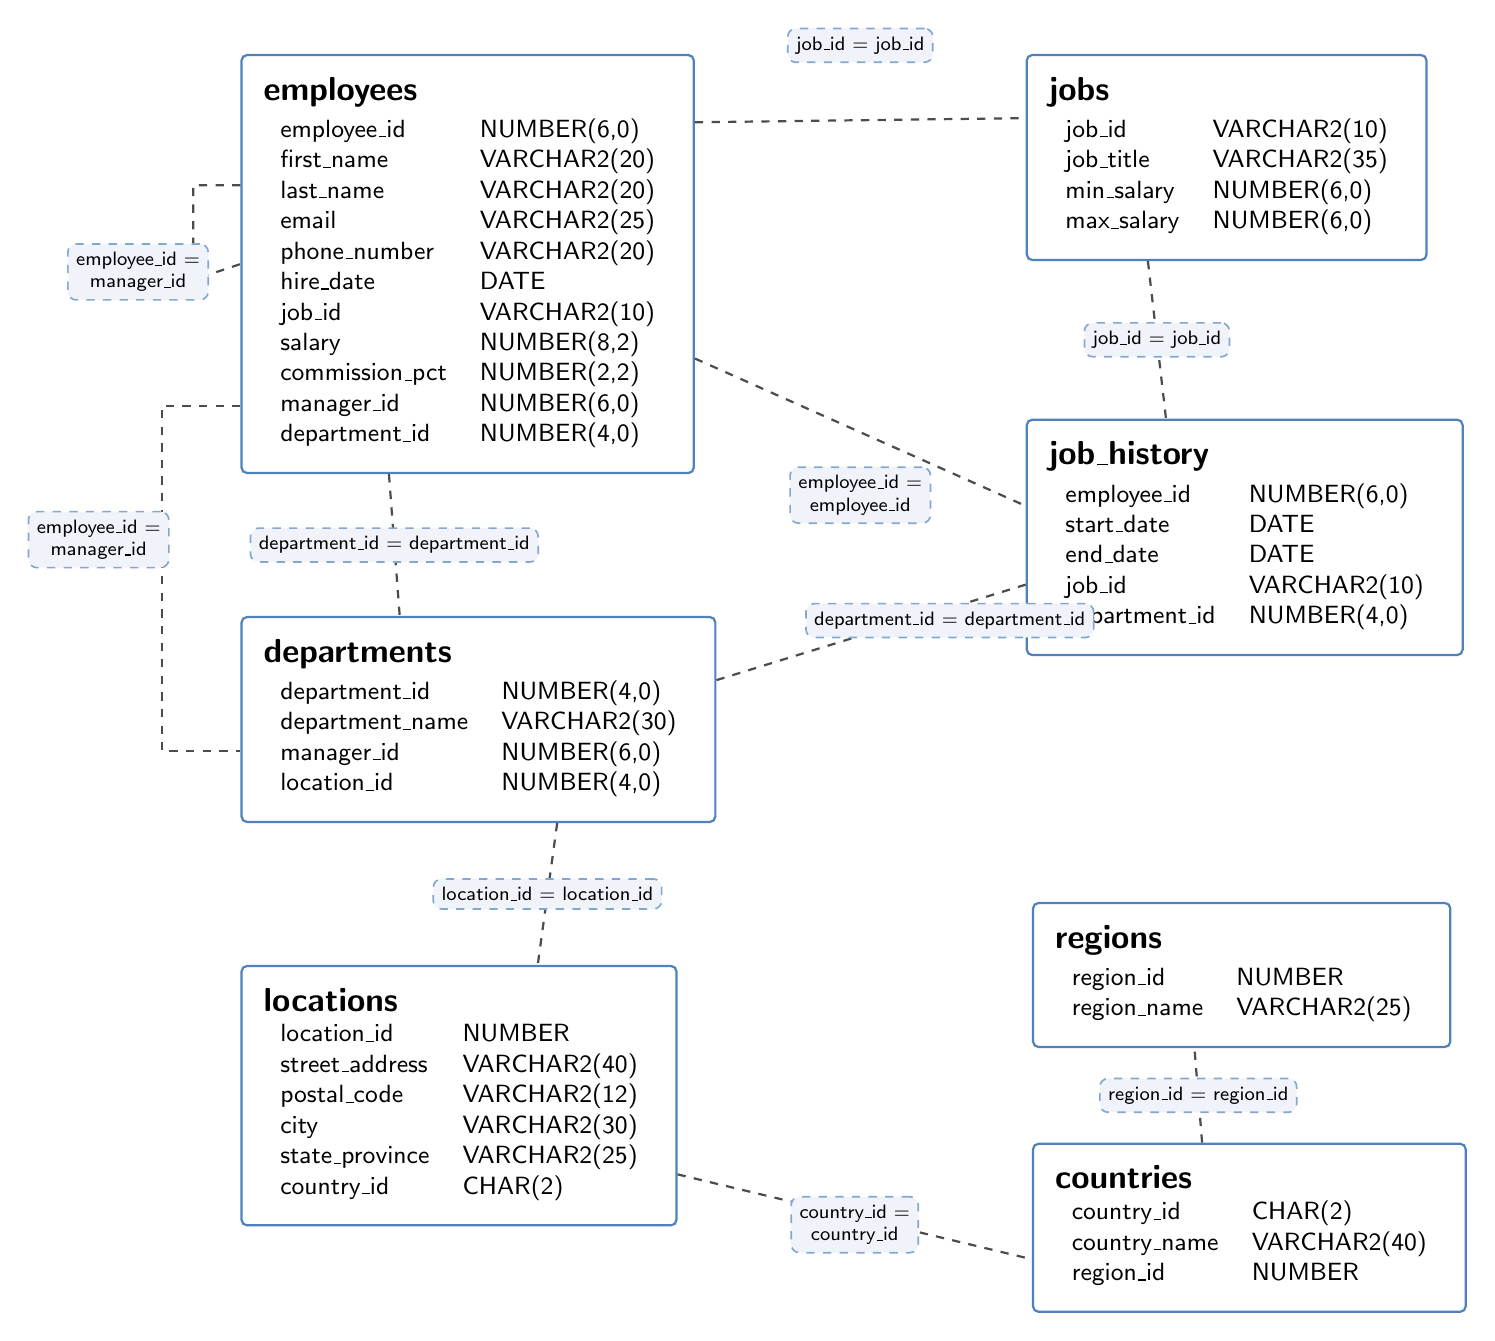
\begin{tikzpicture}[
        >=Stealth,
        line width=0.6pt,
        % Style for the table containers
        table_box/.style={
            draw=borderblue,
            fill=white,
            rounded corners=2pt,
            thick,
            inner sep=8pt,
            font=\sffamily\small,
            align=left
        },
        % Style for the relationship join condition labels
        join_label/.style={
            draw=borderblue!70,
            dashed,
            fill=labelbg,
            rounded corners=3pt,
            font=\sffamily\scriptsize,
            inner sep=3pt,
            align=center
        },
        % Relationship line style
        rel_line/.style={
            draw=black!70,
            dashed,
            thick
        }
    ]

    % ==========================================
    % 1. TABLE DEFINITIONS
    % ==========================================

    % EMPLOYEES
    \node (employees) [table_box] {
        {\large\textbf{employees}}\\[0.6ex]
        \begin{tabular}{ll}
            employee\_id     & NUMBER(6,0) \\
            first\_name      & VARCHAR2(20) \\
            last\_name       & VARCHAR2(20) \\
            email            & VARCHAR2(25) \\
            phone\_number    & VARCHAR2(20) \\
            hire\_date       & DATE \\
            job\_id          & VARCHAR2(10) \\
            salary           & NUMBER(8,2) \\
            commission\_pct  & NUMBER(2,2) \\
            manager\_id      & NUMBER(6,0) \\
            department\_id    & NUMBER(4,0)
        \end{tabular}
    };

    % DEPARTMENTS (Below Employees)
    \node (departments) [table_box, below=1.8cm of employees.south west, anchor=north west] {
        {\large\textbf{departments}}\\[0.6ex]
        \begin{tabular}{ll}
            department\_id   & NUMBER(4,0) \\
            department\_name & VARCHAR2(30) \\
            manager\_id      & NUMBER(6,0) \\
            location\_id     & NUMBER(4,0)
        \end{tabular}
    };

    % LOCATIONS (Below Departments)
    \node (locations) [table_box, below=1.8cm of departments.south west, anchor=north west] {
        {\large\textbf{locations}}\\[0.6ex]
        \begin{tabular}{ll}
            location\_id     & NUMBER \\
            street\_address  & VARCHAR2(40) \\
            postal\_code     & VARCHAR2(12) \\
            city            & VARCHAR2(30) \\
            state\_province  & VARCHAR2(25) \\
            country\_id      & CHAR(2)
        \end{tabular}
    };

    % JOBS (Top Right)
    \node (jobs) [table_box, right=4.2cm of employees.north east, anchor=north west] {
        {\large\textbf{jobs}}\\[0.6ex]
        \begin{tabular}{ll}
            job\_id          & VARCHAR2(10) \\
            job\_title       & VARCHAR2(35) \\
            min\_salary      & NUMBER(6,0) \\
            max\_salary      & NUMBER(6,0)
        \end{tabular}
    };

    % JOB_HISTORY (Middle Right)
    \node (job_history) [table_box, below=2.0cm of jobs.south west, anchor=north west] {
        {\large\textbf{job\_history}}\\[0.6ex]
        \begin{tabular}{ll}
            employee\_id     & NUMBER(6,0) \\
            start\_date      & DATE \\
            end\_date        & DATE \\
            job\_id          & VARCHAR2(10) \\
            department\_id    & NUMBER(4,0)
        \end{tabular}
    };

    % REGIONS (Bottom Right - Top)
    \node (regions) [table_box, right=4.5cm of locations.north east, anchor=north west, yshift=0.8cm] {
        {\large\textbf{regions}}\\[0.6ex]
        \begin{tabular}{ll}
            region\_id       & NUMBER \\
            region\_name     & VARCHAR2(25)
        \end{tabular}
    };

    % COUNTRIES (Bottom Right - Bottom)
    \node (countries) [table_box, below=1.2cm of regions.south west, anchor=north west] {
        {\large\textbf{countries}}\\[0.6ex]
        \begin{tabular}{ll}
            country\_id      & CHAR(2) \\
            country\_name    & VARCHAR2(40) \\
            region\_id       & NUMBER
        \end{tabular}
    };


    % ==========================================
    % 2. RELATIONSHIP LINES AND LABELS
    % ==========================================

    % --- Left side self-loop: employees (manager_id to employee_id) ---
    \draw [rel_line] (employees.west) ++(0, 1.0) -- ++(-0.6, 0) -- ++(0, -1.2) -- (employees.west);
    \node at ($(employees.west) +(-1.3, -0.1)$) [join_label] {employee\_id =\\ manager\_id};

    % --- Left side outer line: employees to departments (manager_id) ---
    \draw [rel_line] (employees.west) ++(0, -1.8) -- ++(-1.0, 0) |- ($(departments.west) + (0, -0.4)$);
    \node at ($(employees.west) +(-1.8, -3.5)$) [join_label] {employee\_id =\\ manager\_id};

    % --- Inner connection: employees to departments (department_id) ---
    \draw [rel_line] (employees.south) ++(-1.0, 0) -- ($(departments.north) + (-1.0, 0)$);
    \node at ($(employees.south) !0.5! (departments.north) + (-1.0, 0)$) [join_label] {department\_id = department\_id};

    % --- Top Horizontal: employees to jobs ---
    \draw [rel_line] (employees.east) ++(0, 1.8) -- ($(jobs.west) + (0, 0.5)$);
    \node at ($(employees.east) !0.5! (jobs.west) + (0, 2.1)$) [join_label] {job\_id = job\_id};

    % --- Vertical: jobs to job_history ---
    \draw [rel_line] (jobs.south) ++(-1.0, 0) -- ($(job_history.north) + (-1.0, 0)$);
    \node at ($(jobs.south) !0.5! (job_history.north) + (-1.0, 0)$) [join_label] {job\_id = job\_id};

    % --- Middle Horizontal: employees to job_history ---
    \draw [rel_line] (employees.east) ++(0, -1.2) -- ($(job_history.west) + (0, 0.4)$);
    \node at ($(employees.east) !0.5! (job_history.west) + (0, -1.2)$) [join_label] {employee\_id =\\ employee\_id};

    % --- Lower Middle Horizontal: departments to job_history ---
    \draw [rel_line] (departments.east) ++(0, 0.5) -- ($(job_history.west) + (0, -0.6)$);
    \node at ($(departments.east) !0.5! (job_history.west) + (1.0, 0.1)$) [join_label] {department\_id = department\_id};

    % --- Lower Vertical: departments to locations ---
    \draw [rel_line] (departments.south) ++(1.0, 0) -- ($(locations.north) + (1.0, 0)$);
    \node at ($(departments.south) !0.5! (locations.north) + (1.0, 0)$) [join_label] {location\_id = location\_id};

    % --- Bottom Horizontal: locations to countries ---
    \draw [rel_line] (locations.east) ++(0, -1.0) -- ($(countries.west) + (0, -0.4)$);
    \node at ($(locations.east) !0.5! (countries.west) + (0, -0.8)$) [join_label] {country\_id =\\ country\_id};

    % --- Bottom Right Vertical: countries to regions ---
    \draw [rel_line] (countries.north) ++(-0.6, 0) -- ($(regions.south) + (-0.6, 0)$);
    \node at ($(countries.north) !0.5! (regions.south) + (-0.6, 0)$) [join_label] {region\_id = region\_id};

    \end{tikzpicture}
\end{center}
\mk{10} \yr{CSE 215 | L-2/T-2 | 2018--19}


%% Q21 — 2019-20 university schema SQL queries (5 queries)
\item Consider the university schema: \texttt{Classroom(building, room\_number, capacity)}, \texttt{department(dept\_name, building, budget)}, \texttt{course(course\_id, title, dept\_name, credits)}, \texttt{instructor(ID, name, dept\_name, salary)}, \texttt{section(course\_id, sec\_id, semester, year, building, room\_number, time\_slot\_id)}, \texttt{teaches(ID, course\_id, sec\_id, semester, year)}, \texttt{student(ID, name, dept\_name, tot\_cred)}, \texttt{takes(ID, course\_id, sec\_id, semester, year, grade)}, \texttt{advisor(s\_ID, i\_ID)}, \texttt{timeslot(time\_slot\_id, day, start\_time, end\_time)}, \texttt{prereq(course\_id, prereq\_id)}. Write SQL queries for the following:
\begin{enumerate}
  \item Find all instructors whose salary is above average for their department.
  \item Find all courses taught in both the Fall 2022 semester and in the Spring 2022 semester.
  \item Find all students who have taken all courses taught by instructor named `John Doe'.
  \item List all departments along with the number of students in each department.
  \item Find the departments that have the lowest average salary.
\end{enumerate}
\mk{20} \yr{CSE 215 | L-2/T-2 | 2019--20}

%% Q22 — 2020-21 Discussion table (topics between users)
\item You have been analysing data from a social networking site and have derived the following relation which captures topics discussed by various users:
\begin{center}
\texttt{Discussion(user1, user2, topic)}
\end{center}
The relation contains a tuple $(u_1, u_2, t)$ every time a user $u_1$ discussed a topic $t$ with user $u_2$. To avoid duplicate entries, \texttt{user1} always precedes \texttt{user2} in alphabetical order.
\begin{enumerate}
  \item Write a SQL query that returns all topics discussed by Pori and Himu but not discussed by Pori and Misir Ali.
  \item Write a SQL query that returns the number of topics discussed by more than 10 pairs of users.
\end{enumerate}
\mk{24} \yr{CSE 215 | L-2/T-2 | 2020--21}

%% Q23 — 2020-21 Conference database CREATE TABLE + queries
\item You are in charge of managing the program committee for an important conference. The \textbf{conference database} stores information about papers submitted to the conference (table Paper), reviewers on the program committee (table Reviewer), and the assignment of reviewers to papers (table Reviews). Each reviewer on the program committee will have to review a set of papers. Each paper will be reviewed by a subset of reviewers. \hfill \textbf{(15)}

\vspace{0.2cm}
\noindent Paper(\underline{pid}, title) \\
Reviewer(\underline{rid}, name) \\
Reviews(rid, pid)
\vspace{0.2cm}

\begin{enumerate}[label=\roman*.]
    \item Declare the conference database using CREATE TABLE. Include the declaration of the keys and maintain the referential integrities as needed. The details are as follows:
    \begin{itemize}
        \item pid is a unique paper identifier and the primary key of the Paper table.
        \item rid is a unique reviewer identifier and the primary key of the Reviewer table.
        \item rid in the Reviews table must be someone mentioned in the Reviewer table. Modifications to Reviewer table that violate this constraint result in:
        \begin{itemize}
            \item[*] the rid in Reviews being set to NULL upon deletion.
            \item[*] update of the rid in Reviews table.
        \end{itemize}
        \item pid in the Review table must be a paper mentioned in the Paper table. Modifications to Paper table that violate this constraint are \textbf{rejected}.
        \item A reviewer is assigned zero or more papers.
        \item A paper is assigned zero or more reviewers.
    \end{itemize}
    
    \item Write a \textbf{SQL query} that finds all papers with fewer than three reviewers assigned to them. The output of the query should be a list paper titles. The result should \textbf{include papers without any reviewers} assigned to them.
    
    \item Write a SQL query that find the reviewers with the most papers assigned to them. \underline{There can be more than one such reviewer.} The output of the query should be a list of reviewer names. A reviewer should be listed if no other reviewer has strictly more papers to review.
\end{enumerate}
\mk{15} \yr{CSE 215 | L-2/T-2 | 2020--21}

%% Q24 — 2021-22 Toys database (5 SQL queries)
\item Consider the Toys database of a retail store. It has the following database schema:

\vspace{0.2cm}
\noindent Toys (\underline{id}, name, color, min\_age, weight, number\_available) \\
Client (\underline{id}, name, age, address, city) \\
Request (\underline{client id}, \underline{toy id})

\vspace{0.2cm}
\noindent The underlined attributes are keys for each relation. The tables contain the following information:

\begin{itemize}
    \item \textit{Toys} records information about all of the toys in the store. Each Toy has a unique integer \textit{id}. Attributes \textit{name} and \textit{color} are strings that describe the toy; \textit{min\_age}, \textit{weight}, and \textit{number\_available} are integers giving the minimum age a child should be to use the toy, the weight of the toy in pounds, and how many are currently available in the store.
    
    \item \textit{Client} stores information about each of the clients. Each client has a unique integer \textit{id}, strings with the client's \textit{name}, \textit{address}, and \textit{city}, and an integer \textit{age}.
    
    \item \textit{Request} has a pair of integers indicating that a particular client has requested a particular toy.
\end{itemize}

\noindent You should assume that all entries in all of the tables are not null. Answer the followings:

\vspace{0.2cm}
\noindent i. Give the name of the clients who do not have any request at the moment for any toys.

\vspace{0.2cm}
\noindent ii. List the name of the toys that has weight more than the average weight of the toys with the same color.

\vspace{0.2cm}
\noindent iii. List the name of the requesting clients who have to wait because the toys are currently unavailable at the store.

\vspace{0.2cm}
\noindent iv. List all of the requests where \textit{age} of the client is less than the \textit{min-age} listed for the Toy. The answer should include the client id, client name, and the toy id. The results should be sorted by client name.

\vspace{0.2cm}
\noindent v. Give the id and name of the "most popular" toy. The most popular toy is the one that has more requests than all others. If there is a tie so there is more than one toy with the maximum number of requests, give the id's and names of all of these toys. They do not need to be in any particular order.

\vspace{0.5cm}
\mk{25} \yr{CSE 215 | L-2/T-2 | 2021--22}

%% Q25 — 2021-22 Product/PC/Laptop schema DML (insert + delete)
\item Consider the following relational database schema:
\begin{center}
\texttt{Product(maker, \underline{model}, type)},\quad \texttt{PC(\underline{model}, speed, ram, hd, price)},\quad \texttt{Laptop(\underline{model}, speed, ram, hd, screen, price)}
\end{center}
Write SQL DML queries to reflect the following:
\begin{enumerate}
  \item Insert the fact that for every PC there is a laptop with the same manufacturer, speed, ram, and hard disk, a 17-inch screen, a model number 1100 greater and a price \$400 more.
  \item Delete all laptops made by a manufacturer that does not make PCs.
\end{enumerate}
\mk{10} \yr{CSE 215 | L-2/T-2 | 2021--22}

%% Q26 — 2021-22 duplicate table copy SQL command
\item Show the SQL command to create a duplicate copy of a table named \texttt{Student}. What would the command be if we only want to copy the schema and not the data of the \texttt{Student} table?
\mk{5} \yr{CSE 215 | L-2/T-2 | 2021--22}

\item You have been tasked to prepare a database for a restaurant, The restaurant has
provided the following report for you.
\begin{center}
  \renewcommand{\arraystretch}{1.3} % Adds a little padding to rows
\begin{tabular}{|l|l|l|l|l|l|l|l|l|l|}
\hline
\multirow{2}{*}{\textbf{Food Item}} & 
\multicolumn{2}{l|}{\makecell[l]{\textbf{Containing Items} \\ \textbf{(For Packages)}}} & 
\multicolumn{3}{l|}{\makecell[l]{\textbf{Ingredients} \\ \textbf{(For Simple Items)}}} & 
\multirow{2}{*}{\makecell[l]{\textbf{Marketed} \\ \textbf{Price}}} & 
\multicolumn{3}{l|}{\textbf{Sales}} \\ \cline{2-6} \cline{8-10}

& \textbf{Simple Item} & \textbf{Qnty} & \textbf{Ingredient} & \makecell[l]{\textbf{Unit} \\ \textbf{Cost}} & \textbf{Qnty} & & \textbf{Buyer} & \textbf{Date} & \textbf{Qnty} \\ \hline

\multirow{5}{*}{Chicken Burger} & & & Chicken Patty & 60 & 1 & \multirow{5}{*}{200} & C1 & 01/02/24 & 2 \\
& & & Lettuce & 30 & 0.02 & & C3 & 02/02/24 & 4 \\
& & & Pickle & 5 & 4 & & C8 & 02/02/24 & 1 \\
& & & Mayonnaise & 100 & 0.02 & & C1 & 03/02/24 & 3 \\
& & & Sause & 70 & 0.01 & & & & \\ \hline

\multirow{3}{*}{Fried Rice} & & & Raw Rice & 50 & 0.1 & \multirow{3}{*}{80} & C4 & 02/02/24 & 1 \\
& & & Egg & 7 & 1 & & C9 & 04/02/24 & 2 \\
& & & Oil & 500 & 0.005 & & & & \\ \hline

\multirow{4}{*}{Set Menu 1} & Fried Rice & 1 & & & & \multirow{4}{*}{500} & C2 & 01/02/24 & 3 \\
& Vegetable & 1 & & & & & C4 & 03/02/24 & 1 \\
& Chicken Steak & 1 & & & & & C1 & 04/02/24 & 4 \\
& & & & & & & C1 & 05/02/24 & 2 \\ \hline

\end{tabular}
\end{center}
In the above table, “Qnty” means “quantity of the item”.
Now, create a relational schema, find its functional dependencies and normalize the
schema. Write down all normalized forms up to BCNF, (1NF, 2NF, 3NF, BCNF).

%% Q27 — 2022-23 restaurant SQL view (production cost) + monthly profit
 Using the schema created for the restaurant database in:
\begin{enumerate}
  \item Write a SQL query to create a view that contains the total cost of production of each food item. Cost of production for simple items depends on the total cost of ingredients (unit cost $\times$ quantity used); for packages, it depends on the total cost of the containing simple items.
  \item Using the schema and view above, find the monthly profit for each food item where profit $=$ (marketed price $-$ cost of production) $\times$ quantity sold in the month.
\end{enumerate}
\mk{20} \yr{CSE 215 | L-2/T-1 | 2022--23}

%% Q28 — 2023-24 roles and privileges (Admin, SuperAdmin, U1 U2 U3)
\item Why are roles used for assigning privileges to users? Create three users U1, U2, and U3 and assign them INSERT and UPDATE privileges on tables T1 and T2 by assigning them a role of ``Admin''. Then transfer these privileges to another role named ``SuperAdmin''. Finally, revoke the UPDATE privilege from ``Admin''.
\mk{10} \yr{CSE 215 | L-2/T-1 | 2023--24}

%% Q29 — 2023-24 EMPLOYEE/JOB/DEPARTMENT/JOB_HISTORY SQL queries (5 queries)
\item Consider the following schema:
\begin{center}
\begin{tabular}{l}
\texttt{EMPLOYEE(EMPLOYEEID, LASTNAME, FIRSTNAME, PHONE, HIREDATE, JOBID, SALARY, DEPARTMENTID)}\\
\texttt{JOB(JOBID, JOBTITLE, MINSALARY, MAXSALARY)}\\
\texttt{DEPARTMENT(DEPARTMENTID, DEPARTMENTNAME, MANAGERID)}\\
\texttt{JOB\_HISTORY(EMPLOYEEID, JOBID, DEPARTMENTID, STARTDATE, ENDDATE)}
\end{tabular}
\end{center}
Write SQL to implement the following queries:
\begin{enumerate}
  \item For each employee, find the total number of employees hired before him/her and those hired after him/her. Print employee last name, total employees hired before, and total employees hired after.
  \item Print the last name of the employees who never changed their job or department.
  \item Print the last name of the employees and the difference between their salary and the maximum salary of their department, such that the difference is not more than 5000.
  \item For each department, print the department name, corresponding manager's last name, and the number of employees working under that manager in that department.
  \item Print the last name of employees who get a higher salary than the average salary of their department. Also print the difference between their salary and the department average.
\end{enumerate}
\mk{25} \yr{CSE 215 | L-2/T-1 | 2023--24}

%% Q30 — 2024-25 Planet/Moon SQL: function total_moons() + LIKE pattern
\item Consider the following relational database schema:
\begin{center}
\texttt{Planet(\underline{planet\_id}, name, type, distance\_sun\_au)},\quad --- planet-id is the primary key.
\\ \texttt{Moon(\underline{moon\_id}, name, planet\_id, diameter\_km)}, \ moon_id is the primary key, and planet_id is a foreign key referencing Planet(planet_id). 
\end{center}
\begin{enumerate}
  \item Write an SQL function \texttt{total\_moons()} that returns a single integer representing the total number of moons possessed by all planets. Then write the SQL statement to call the function.
  \item Find the names of all planets whose name contains a substring that starts with ``Ma'', then has exactly two unknown characters, and ends with ``s''.
\end{enumerate}
\mk{12} \yr{CSE 215 | L-2/T-1 | 2024--25}

%% Q31 — 2024-25 employee/works/company/manages SQL DML + trigger
\item Consider the following relational database schema:
\begin{center}
\texttt{employee(employee\_name, street, city)},\quad \\\texttt{works(employee\_name, company\_name, salary)},\\
\texttt{company(company\_name, city)},\quad \\\texttt{manages(employee\_name, manager\_name)}
\end{center}
Write SQL statements for the following:
\begin{enumerate}
  \item Give a 20\% salary rise to employees who are managers.
  \item Delete all tuples in the \texttt{works} relation for employees of the company ``Sonali Bank''. 
  Note that works.employee_name is a foreign key referencing employee(employee_name),
 manages.employee_name is a foreign key referencing employee(employee_name),
 manages.manager_name is a foreign key referencing employee(employee_name) .
  \item Design a trigger such that whenever a manager's salary is updated, all employees managed by that manager receive a 10\% salary increase.
\end{enumerate}
\mk{18} \yr{CSE 215 | L-2/T-1 | 2024--25}

%% Q32 — 2024-25 integrity constraints CREATE TABLE from real-life scenario
\item Create a table in SQL from a real-life scenario where you need to apply all types of integrity constraints.
\mk{10} \yr{CSE 215 | L-2/T-1 | 2024--25}

\end{enumerate}

%%──────────────────────────────────────────────────────────────────────
\subtopic{cB}{Relational Algebra}
\label{sub:s3-relalg}

\begin{enumerate}

%% Q1
\item Using the schema below, express the following queries using relational algebra:
\begin{center}
\begin{tabular}{l}
\texttt{Product(\underline{pid}, name, price, category, year, maker\_cid)}\\
\texttt{Purchase(\underline{buyer\_ssn}, \underline{seller\_ssn}, store, pid)}\\
\texttt{Company(\underline{cid}, name, stock\_price, country)}\\
\texttt{Person(\underline{ssn}, name, phone\_number, city)}
\end{tabular}
\end{center}
\begin{enumerate}
  \item Find names of people who bought Indian products and live in Gulshan.
  \item Find people who bought stuff from Alam or bought products from a company whose stock price is more than BDT 2500.
\end{enumerate}
\mk{8} \yr{CSE 215 | L-3/T-1 | 2010--11}

%% Q2
\item Using the schema below, express the following queries using relational algebra:
\begin{center}
\begin{tabular}{l}
\texttt{Emp(\underline{eno}, ename, title, city)},\quad
\texttt{Proj(\underline{pno}, pname, budget, city)}\\
\texttt{Works(\underline{eno}, \underline{pno}, resp, dur)},\quad
\texttt{Pay(\underline{title}, salary)}
\end{tabular}
\end{center}
\begin{enumerate}
  \item Find names of employees whose salary is more than \$1000.
  \item List all projects where at least one person with `Programmer' title is working on it. (A project name may appear more than once.)
\end{enumerate}
\mk{10} \yr{CSE 303 | L-3/T-1 | 2011--12}

%% Q3
\item Consider the following relational schema:
\begin{center}
\begin{tabular}{l}
\texttt{employee(\underline{emp\_no}, name, office, age)}\\
\texttt{books(\underline{isbn}, title, author, publisher)}\\
\texttt{loan(\underline{empno}, \underline{isbn}, date)}
\end{tabular}
\end{center}
Answer the following queries in relational algebra:
\begin{enumerate}
  \item Find the names of employees who have borrowed a book published by McGraw-Hill.
  \item Find the names and ages of employees who have borrowed all books written by Carl Hamacher.
  \item Find the names of employees who have borrowed more than five different books published by Pearson Education.
  \item For each publisher, find the names of employees who have borrowed more than five books of that publisher.
  \item Find the titles and authors of the books that have been borrowed by Peter Hart.
\end{enumerate}
\mk{25} \yr{CSE 303 | L-3/T-1 | 2012--13}

%% Q4 — 2015-16 Flight/Route schema
\item Consider the following schema:
\begin{center}
\begin{tabular}{l}
\texttt{Route(\underline{FN}, DC, AC, DI, SD, SA, PM)}\\
\texttt{Flight(\underline{FN}, \underline{DT}, NP, AD, AA)}\\
\texttt{Plane(\underline{PM}, CA, TP)}
\end{tabular}
\end{center}
\textit{(FN=flight number, DC=departure city, AC=arrival city, DI=distance, SD=sched.\ depart, SA=sched.\ arrive, PM=plane model, DT=date, NP=no.\ of passengers, AD=actual depart, AA=actual arrive, CA=capacity, TP=type)}

Translate the following queries into relational algebra:
\begin{enumerate}
  \item Which flights have at least 50 passengers on board and arrived more than 30 minutes late?
  \item What are the departure and arrival cities of all flights on October 10th that were completely full?
  \item What are the plane types that travel between BOSTON (BOS) and FRANCISCO (SFO)?
  \item Which flights departed late but arrived without any delay?
\end{enumerate}


\begin{center}
\renewcommand{\arraystretch}{1.1} % Slightly improve row spacing

\begin{tabular}{cl}

% ==========================================
% ROUTE TABLE
% ==========================================
\textbf{ROUTE} & 
\begin{tabular}{ccccccc}
\shortstack{flight \\ number \\ (FN)} & 
\shortstack{from \\ city \\ (FC)} & 
\shortstack{to \\ city \\ (TC)} & 
\shortstack{distance \\ in miles \\ (DI)} & 
\shortstack{scheduled \\ departure \\ time \\ (SD)} & 
\shortstack{scheduled \\ arrival \\ time \\ (SA)} & 
\shortstack{ \\ plane \\ (PM)} \\
\hline
1384 & ROC & BOS & 325 & 0650 & 0810 & F101 \\
1205 & BOS & ROC & 325 & 1730 & 1900 & F101 \\
 110 & BOS & LAX & 3250 & 0900 & 1040 & L1011 \\
 398 & LAX & SFO & 340 & 1120 & 1210 & 757 \\
 124 & SFO & BOS & 3180 & 1400 & 2310 & L1011 \\
 448 & BOS & DCA & 340 & 0700 & 0830 & 737 \\
 540 & DCA & BOS & 340 & 1900 & 2030 & 737 \\
\end{tabular} \\
\multicolumn{2}{c}{} \\ % Spacing between tables
\multicolumn{2}{c}{} \\

% ==========================================
% FLIGHT TABLE
% ==========================================
\textbf{FLIGHT} & 
\begin{tabular}{ccccc}
\shortstack{flight \\ number \\ (FN)} & 
\shortstack{ \\ date \\ (DT)} & 
\shortstack{number of \\ passengers \\ (NP)} & 
\shortstack{actual \\ departure \\ time \\ (AD)} & 
\shortstack{actual \\ arrival \\ time \\ (AA)} \\
\hline
1384 & 2000-10-09 & 40 & 0650 & 0800 \\
1384 & 2000-10-10 & 12 & 0730 & 0842 \\
1384 & 2000-10-11 & 30 & 0700 & 0815 \\
1205 & 2000-10-09 & 42 & 1735 & 1900 \\
1205 & 2000-10-10 &  8 & 1730 & 1855 \\
1205 & 2000-10-11 & 20 & 1810 & 1932 \\
 110 & 2000-10-10 & 403 & 0940 & 1115 \\
 110 & 2000-10-11 & 385 & 0905 & 1035 \\
 398 & 2000-10-09 & 148 & 1150 & 1220 \\
 398 & 2000-10-10 & 95 & 1125 & 1210 \\
 124 & 2000-10-09 & 150 & 1500 & 2350 \\
 124 & 2000-10-10 & 414 & 1410 & 2310 \\
\end{tabular} \\
\multicolumn{2}{c}{} \\ % Spacing between tables
\multicolumn{2}{c}{} \\

% ==========================================
% PLANE TABLE
% ==========================================
\textbf{PLANE} & 
\begin{tabular}{ccc}
\shortstack{model \\ (PM)} & 
\shortstack{capacity \\ (CA)} & 
\shortstack{type \\ (TP)} \\
\hline
737 & 120 & jet \\
747 & 460 & jet \\
757 & 200 & jet \\
L1011 & 440 & jet \\
F101 & 45 & prop \\
\end{tabular} \\

\end{tabular}
\end{center}

\mk{15} \yr{CSE 303 | L-3/T-1 | 2015--16}

%% Q5 — 2014-15 Suppliers/Parts/Catalog schema
\item Consider the following schema:
\begin{center}
\begin{tabular}{l}
\texttt{Suppliers(sid: integer, sname: string, address: string)}\\
\texttt{Parts(pid: integer, pname: string, color: strign)}\\
\texttt{Catalog(sid: integer, pid: integer, cost: real)}
\end{tabular}
\end{center}
Write relational algebra expressions for the following:
\begin{enumerate}
  \item Find the sids of suppliers who supply some red or green part.
  \item Find the sids of suppliers who supply some red parts and are at the address `221 Packer Street'.
  \item Find the sids of suppliers who supply some red parts and some green parts.
  \item Find the sids of suppliers who supply every part.
\end{enumerate}
\mk{20} \yr{CSE 303 | L-3/T-1 | 2014--15}

%% Q6 — 2013-14 Employee/Job/Department schema
\item Consider the following schema:
\begin{center}
\begin{tabular}{l}
\texttt{EMPLOYEE(\underline{EMPLOYEEID}, LASTNAME, FIRSTNAME, PHONE, HIREDATE, JOBID, SALARY, DEPARTMENT)}\\
\texttt{JOB(\underline{JOBID}, JOBTITLE, MINSALARY, MAXSALARY)}\\
\texttt{DEPARTMENT(\underline{DEPARTMENTID}, DEPARTMENTNAME, MANAGERID)}
\end{tabular}
\end{center}
Write relational algebra expressions for the following:
\begin{enumerate}
  \item List the average salary of each department.
  \item List the FIRSTNAME and JOBTITLE of employee `John'.
  \item Increase all salaries more than 10000 by 5\% and less than 10000 by 4\%.
  \item Delete all employees from the EMPLOYEE table who earn less than 1000 as salary.
\end{enumerate}
\mk{20} \yr{CSE 303 | L-3/T-1 | 2013--14}

%% Q7 — 2016-17 customer/account/transaction schema
\item Given three relations:
\begin{center}
\begin{tabular}{l}
\texttt{customer(\underline{customer\_id}, name, street, city)}\\
\texttt{account(\underline{account\_number}, type, balance)}\\
\texttt{transaction(\underline{customer\_id}, \underline{account\_number}, date, amount)}
\end{tabular}
\end{center}
\begin{enumerate}
  \item Write a relational algebra expression using Cartesian product to find customer\_id, date and amount of all transactions made by customer id ``C005''.
  \item Rewrite the expression of (i) using natural join.
  \item Write the equivalent relational algebra expression for the following SQL:
\begin{lstlisting}[language=SQL]
SELECT a.customer_id, b.account_number, name, street, city
FROM customer AS a, account AS b, transaction AS c
WHERE a.customer_id = c.customer_id
  AND b.account_number = c.account_number
  AND date = '01-JAN-2017'
  AND amount > 10000;
\end{lstlisting}
\end{enumerate}
\mk{20} \yr{CSE 303 | L-3/T-1 | 2016--17}

%% Q8 — 2017-18 Manufacturer/Laptop/Printer schema
\item Consider the following schemas:
\begin{center}
\begin{tabular}{l}
\texttt{Manufacturer(\underline{man\_id}, name, address)}\\
\texttt{Laptop(\underline{model}, man\_id, speed, ram, hd, screen, price)}\\
\texttt{Printer(\underline{model}, man\_id, is\_color, type, price)}
\end{tabular}
\end{center}
Write relational algebra expressions for:
\begin{enumerate}
  \item Find the model and speeds of each laptop manufactured by ``Dell''.
  \item Find the sorted list of names of the manufacturers that produce at least three different models of laptops.
\end{enumerate}
\mk{10} \yr{CSE 215 | L-2/T-2 | 2017--18}

%% Q9 — 2018-19 Sonali Bank schema
\item Consider the following schema of Sonali Bank Limited:
\begin{center}
\begin{tabular}{l}
\texttt{customer(\underline{customer\_id}, customer\_name, customer\_address)}\\
\texttt{account(\underline{account\_id}, account\_type, account\_branch, account\_balance)}\\
\texttt{branch(\underline{branch\_routing\_number}, branch\_name)}\\
\texttt{transaction(\underline{account\_id}, transaction\_amount, transaction\_date)}\\
\texttt{loan(\underline{loan\_id}, customer\_id, loan\_amount)}
\end{tabular}
\end{center}
Notice that the attribute account_branch of table account is a foreign key referencing
the primary key branch_routing number from table branch. On the other hand,
the attribute account_id of table account is a foreign key referencing the primary key
customer_id from table customer.
\begin{enumerate}
  \item Write a relational algebra expression using Cartesian product to find customers' names and their corresponding loan amounts who have a ``savings'' type account at the branch named ``BUET Br.''.
  \item Write the equivalent relational algebra expression for the following SQL:
\begin{lstlisting}[language=SQL]
SELECT c.customer_name, a.account_id, t.transaction_amount
FROM customer c, account a, transaction t
WHERE c.customer_id = a.account_id
  AND a.account_id = t.account_id
  AND t.transaction_date = '01-JAN-2020'
  AND t.transaction_amount > 5000;
\end{lstlisting}
\end{enumerate}
\mk{20} \yr{CSE 215 | L-2/T-2 | 2018--19}

%% Q10 — 2019-20 university schema RA queries (5 queries)
\item Given the university schema: \texttt{Classroom(building, room\_number, capacity)}, \texttt{department(dept\_name, building, budget)}, \texttt{course(course\_id, title, dept\_name, credits)}, \texttt{instructor(ID, name, dept\_name, salary)}, \texttt{section(course\_id, sec\_id, semester, year, building, room\_number, time\_slot\_id)}, \texttt{teaches(ID, course\_id, sec\_id, semester, year)}, \texttt{student(ID, name, dept\_name, tot\_cred)}, \texttt{takes(ID, course\_id, sec\_id, semester, year, grade)}, \texttt{advisor(s\_ID, i\_ID)}, \texttt{timeslot(time\_slot\_id, day, start\_time, end\_time)}, \texttt{prereq(course\_id, prereq\_id)}. Write the following queries in relational algebra:
\begin{enumerate}
  \item Find the ID and name of each instructor in the Physics department.
  \item Find the ID and name of each instructor in a department located in the building `Watson'.
  \item Find all the courses taught in the Fall 2022 semester but not in Spring 2022 semester.
  \item Find the ID and name of those instructors who earn more than the instructors in the Physics department.
  \item Find the ID and name of each student who has not taken any course section in the year 2022.
\end{enumerate}
\mk{15} \yr{CSE 215 | L-2/T-2 | 2019--20}

%% Q11 — 2020-21 show pi_a(R intersect S) != pi_a(R) intersect pi_a(S)
\item Using an example, show that $\pi_a(R \cap S) \neq \pi_a(R) \cap \pi_a(S)$.
\mk{5} \yr{CSE 215 | L-2/T-2 | 2020--21}

%% Q12 — 2021-22 min/max tuples for RA expressions (bags)
\item Suppose we have two relations $A$ and $B$ with the same set of attributes. Relation $A$ has $n_a$ tuples and relation $B$ has $n_b$ tuples. For each of the following relational algebra expressions, give the minimum and maximum number of tuples that can appear in the result. Assume that the produced results are bags, not sets.
\begin{enumerate}
  \item $A \cap B$
  \item $\sigma_c(A) - B$
  \item $A \cup B$
  \item $A \bowtie_L B$, where $\bowtie_L$ is the left outer join
\end{enumerate}
\mk{8} \yr{CSE 215 | L-2/T-2 | 2021--22}

%% Q13 — 2022-23 admission exam schema RA queries (3 queries)
\item A school has prepared a database to manage admission tests. The examinees are given
roll numbers and assigned to specific rooms for the exam. The test contains 10 questions.
Each question is marked by two examiners to ensure fairness and correctness. An
absentee list is kept to ensure no script goes missing. The schema for the database is as:
follows:
\begin{center}
\begin{tabular}{l}
\texttt{Room(\underline{Room\_No}, Floor, Capacity)}\\
\texttt{Examinee(\underline{Roll\_No}, Name, Address, Date\_of\_Birth, Room\_No)}\\
\texttt{Evaluation(\underline{Roll\_No},\underline{Question\_No},\underline{Examiner}, Marks)}\\
\texttt{Absentee(\underline{Roll\_No})}
\end{tabular}
\end{center}
Write queries using relational algebra to compute the following:
\begin{enumerate}
\item The students should be assigned to the rooms in a manner that all the “Roll No”s in the”
room are sequential (e.g., if a room has 10 examinees and the lowest Roll No in that room
is 501, then “Roll No”s 502, 503, ...,510 should be assigned to that room). Find the
rooms that violate this condition.
\item We need to check if all scripts have been correctly evaluated, i.e., all examinees'
answers to all questions have been evaluated by exactly two teachers. Find out the Roll
No and Question No of the students that have not got correctly evaluated. Please note
that only the examinees that are present in the exam should be considered here.
\item The marks given by two examiners can only be at most 2 marks apart (i.e., for a
student's answer to a specific question, the two marks by the two examiners should not
differ by more than 2). Find the Roll No and Question No for which two examiners'
marks differ by more than 2.
\end{enumerate}
\mk{30} \yr{CSE 215 | L-2/T-1 | 2022--23}

%% Q14 — 2023-24 Suppliers/Parts/Catalog RA (5 queries)
\item Consider the following schema:
\begin{center}
\texttt{Suppliers(\underline{sid}, sname, address)},\quad \texttt{Parts(\underline{pid}, pname, color)},\quad \texttt{Catalog(\underline{sid}, \underline{pid}, cost)}
\end{center}
Write relational algebraic expressions for the following:
\begin{enumerate}
  \item Find the names of suppliers who supply more than 10 parts.
  \item Find the sids of suppliers who supply some red or green part.
  \item Find the sids of suppliers who supply some red part or are located at 221 Packer Street.
  \item Find the sids of suppliers who supply some red part with each part's cost more than 100 taka.
  \item Find the sids of suppliers who supply every part.
\end{enumerate}
\mk{25} \yr{CSE 215 | L-2/T-1 | 2023--24}

%% Q15 — 2024-25 Instructor + Teaches RA: compute output of 3 expressions
\item Consider the relations \texttt{Instructor} and \texttt{Teaches} below. Compute the output of the following:
\begin{enumerate}
  \item $\Pi_{name}(\sigma_{salary < 900000}(\text{Instructor}))$
  \item $\sigma_{year=2024}(\sigma_{\text{Instructor.id}=\text{Teaches.id}}(\text{Instructor} \times \text{Teaches}))$
  \item $\Pi_{name}(\text{Instructor} \bowtie_{\text{Instructor.id}=\text{Teaches.id}} \text{Teaches})$
\end{enumerate}
\begin{center}
\small
\begin{tabular}{llll}
\toprule
\multicolumn{4}{c}{\textbf{Instructor}}\\
\textbf{id} & \textbf{name} & \textbf{dept\_name} & \textbf{salary}\\
\midrule
1 & Alice & CSE     & 950000\\
2 & Bob   & Physics & 2300000\\
3 & Carol & CSE     & 720000\\
4 & David & Math    & 2200000\\
5 & Eve   & CSE     & 2500000\\
\bottomrule
\end{tabular}
\quad
\begin{tabular}{llll}
\toprule
\multicolumn{4}{c}{\textbf{Teaches}}\\
\textbf{id} & \textbf{course\_id} & \textbf{semester} & \textbf{year}\\
\midrule
1 & CS101 & Fall   & 2023\\
1 & CS102 & Spring & 2024\\
2 & PH201 & Fall   & 2023\\
3 & CS101 & Fall   & 2023\\
5 & CS201 & Fall   & 2023\\
\bottomrule
\end{tabular}
\end{center}
\mk{9} \yr{CSE 215 | L-2/T-1 | 2024--25}

\end{enumerate}

%%──────────────────────────────────────────────────────────────────────
\subtopic{cB}{Joins}
\label{sub:s3-joins}

\begin{enumerate}

%% Q1
\item Define natural joins and outer joins.
\mk{7} \yr{CSE 215 | L-3/T-1 | 2010--11}

%% Q2
\item Distinguish between `cross join', `natural join' and `outer joins'. When (left or right) outer joins are useful? Give an example.
\mk{10} \yr{CSE 303 | L-3/T-1 | 2011--12}

%% Q3 — 2016-17
\item Explain the application of left, right and full outer joins with examples.
\mk{15} \yr{CSE 303 | L-3/T-1 | 2016--17}

\end{enumerate}

%%──────────────────────────────────────────────────────────────────────
\subtopic{cB}{Constraints, Assertions \& Triggers}
\label{sub:s3-constraints}

\begin{enumerate}

%% Q1
\item A database schema consists of four relations:
\begin{center}
\begin{tabular}{l}
\texttt{Product(maker, model, type)}\\
\texttt{PC(model, speed, ram, hd, price)}\\
\texttt{Laptop(model, speed, ram, hd, screen, price)}\\
\texttt{Printer(model, color, type, price)}
\end{tabular}
\end{center}
\begin{enumerate}
\item Write the following check constraints (using the PC/Laptop/Printer schema):
\begin{enumerate}
  \item The model number of a product must be a 7-digit number.
  \item A PC with a processor speed less than 2.0 GHz must have at least 512 MB RAM or sell for less than \$800.
\end{enumerate}
\mk{5} \yr{CSE 303 | L-3/T-1 | 2011--12}

\item Write the following assertions:
\begin{enumerate}
  \item The price of a laptop must be larger than the average price of PCs made by the same manufacturer.
  \item A manufacturer of a PC must also make Laptop(s).
  \item If a PC has a greater processor speed than a laptop then the PC must also have a higher price than the laptop.
\end{enumerate}
\mk{15} \yr{CSE 303 | L-3/T-1 | 2011--12}
\end{enumerate}

%% Q3
\item What are the different policies of maintaining referential integrity? Discuss them with examples.
\mk{10} \yr{CSE 303 | L-3/T-1 | 2012--13}

%% Q4
\item What are the differences between \texttt{UNIQUE} and \texttt{PRIMARY KEY} constraints in SQL?
\mk{5} \yr{CSE 303 | L-3/T-1 | 2012--13}

%% Q5
\item Give an example of a \texttt{CHECK} constraint and discuss why it is used.
\mk{5} \yr{CSE 303 | L-3/T-1 | 2012--13}

%% Q6 — Materialized View and Triggers
\item What is a Materialized View? Discuss four instances when a trigger can be applied.
\mk{10} \yr{CSE 303 | L-3/T-1 | 2013--14}

\variant{2014--15: ``What is a Materialized View? Discuss the restrictions on triggers in brief.''}

%% Q7 — 2017-18 Trigger on netWorth constraint
\item Consider the schema \texttt{MovieExec(name, address, cert\#, netWorth)}. We want to prevent the average net worth of movie executives from dropping below \$50,000. Write a trigger that checks this constraint before each update to the \texttt{netWorth} column and, if violated, sets the value of \texttt{netWorth} to the minimum amount required to satisfy the constraint.
\mk{10} \yr{CSE 215 | L-2/T-2 | 2017--18}

%% Q8 — 2019-20 referential integrity vs foreign key + UPDATE/DELETE policies
\item What is the difference between referential integrity constraint and foreign key constraint? What are the three different policies for UPDATE and DELETE that can be mentioned for maintaining referential integrity? Among these, which one is more suitable for UPDATE, and which one is more suitable for DELETE? Why?
\mk{10} \yr{CSE 215 | L-2/T-2 | 2019--20, 2015--16}

%% Q9 — 2020-21 UNIQUE constraint replaced by CHECK
\item Consider the following table definition:
\begin{lstlisting}
CREATE TABLE MyTable(
    ...
    head INT UNIQUE,
    ...
);
\end{lstlisting}
Replace the above \texttt{UNIQUE} constraint using a \texttt{CHECK} constraint.
\mk{15} \yr{CSE 215 | L-2/T-2 | 2020--21}

%% Q10 — 2020-21 triggers for Product/Laptop schema
\item Consider the following two schemas:
\begin{center}
\texttt{Product(maker, model, type)},\quad \texttt{Laptop(model, speed, ram, hd, screen, price)}
\end{center}
Write necessary triggers to implement the following constraints:
\begin{enumerate}
  \item \texttt{speed}, \texttt{ram}, \texttt{hd}, \texttt{screen} and \texttt{price} cannot be negative.
  \item When a Laptop model is deleted, that model must also be deleted from the \texttt{Product} table.
\end{enumerate}
 \mk{12} \yr{CSE 215 | L-2/T-2 | 2020--21}

%% Q11 — 2021-22 UNIQUE vs PRIMARY KEY
\item What is the difference between a \texttt{UNIQUE} key and a \texttt{PRIMARY KEY}?
\mk{3} \yr{CSE 215 | L-2/T-2 | 2021--22}

%% Q12 — 2021-22 constraints on Product/PC/Laptop/Printer schema
\item Consider the following relational database schema:
\begin{center}
\texttt{Product(maker, \underline{model}, type)},\quad \texttt{PC(\underline{model}, speed, ram, hd, price)},\\
\texttt{Laptop(\underline{model}, speed, ram, hd, screen, price)},\quad \texttt{Printer(\underline{model}, color, type, price)}
\end{center}
The \textit{Product} relation gives the manufacturer, model number and type (PC, laptop, or printer) of various products. model numbers are unique over all manufacturers and product types. The \textit{PC} relation gives for each model number that is a PC the speed (of the processor, in gigahertz), the amount of RAM (in megabytes), the size of the hard disk (in gigabytes), and the price. The \textit{Laptop} relation is similar, except that the screen size (in inches) is also included. The \textit{Printer} relation records for each printer model whether the printer produces color output ('T', if so; 'F' otherwise), the process type (laser or ink-jet, typically), and the price.
Write necessary constraints to implement the following (answer each independently):
\begin{enumerate}
  \item \texttt{speed}, \texttt{ram}, \texttt{hd}, \texttt{screen} and \texttt{price} cannot be negative.
  \item A model of a product must also be the model of a PC, a laptop, or a printer.
  \item A laptop with a screen size less than 15 inches must have at least a 40 GB hard disk or sell for less than \$1000.
  \item No manufacturer of PCs may also make laptops.
  \item If a laptop has a larger main memory than a PC, then the laptop must also have a higher price than the PC.
  \item A manufacturer of a PC also makes a laptop with at least as great a processor speed.
\end{enumerate}
\mk{24} \yr{CSE 215 | L-2/T-2 | 2021--22}

%% Q13 — 2023-24 trigger for prerequisite course check on registration
\item Consider the following schema:
\begin{center}
\begin{tabular}{l}
\texttt{Student(\underline{Ssn}, Name)},\quad \texttt{TakenCourses(\underline{Ssn}, \underline{CourseNo})}\\
\texttt{Register(\underline{Ssn}, \underline{CourseNo})},\quad \texttt{Course(\underline{CourseNo}, Name, Year, Term)}\\
\texttt{PreRequisite(\underline{CourseNo}, \underline{ReqCourseNo})}
\end{tabular}
\end{center}
Table \texttt{TakenCourses} manages courses a student has previously taken. Write a trigger to check if a student has taken the prerequisite courses when he/she registers for a new course. If a prerequisite course has not been taken, the registration should fail and an appropriate message should be displayed.
\mk{10} \yr{CSE 215 | L-2/T-1 | 2023--24}

\end{enumerate}

%%──────────────────────────────────────────────────────────────────────
\subtopic{cB}{Functions and Procedures}
\label{sub:s3-funcs}

\begin{enumerate}

%% Q1 — 2016-17 constructor functions
\item Write constructor functions for the car rental SQL:99 schema (Trucks, Sports car, Bus) and insert statement to insert data into the tables.
\mk{10} \yr{CSE 303 | L-3/T-1 | 2016--17}

%% Q2 — 2017-18 stored procedure
\item Consider the following schema:
\begin{center}
\begin{tabular}{l}
\texttt{Movie(\underline{title}, \underline{year}, filmType, inColor, studioId)}\\
\texttt{Studio(\underline{studioId}, name, address)}
\end{tabular}
\end{center}
Write a stored procedure that takes as input the name of a studio and a year, then counts and prints the number of black and white movies produced by that studio in the specified year.
\mk{10} \yr{CSE 215 | L-2/T-2 | 2017--18}

%% Q3 — 2018-19 IncreaseOrDecrease procedure
\item Write a procedure named \texttt{IncreaseOrDecrease} which takes an employee id as input. If the salary of the employee is greater than the average salaries of all departments except their own, but less than the average salary of their own department, the procedure increases the salary by 10\%. Otherwise it decreases by 5\%. During execution it prints ``Increasing Salary'' or ``Decreasing Salary'' accordingly.

\begin{center}
  
    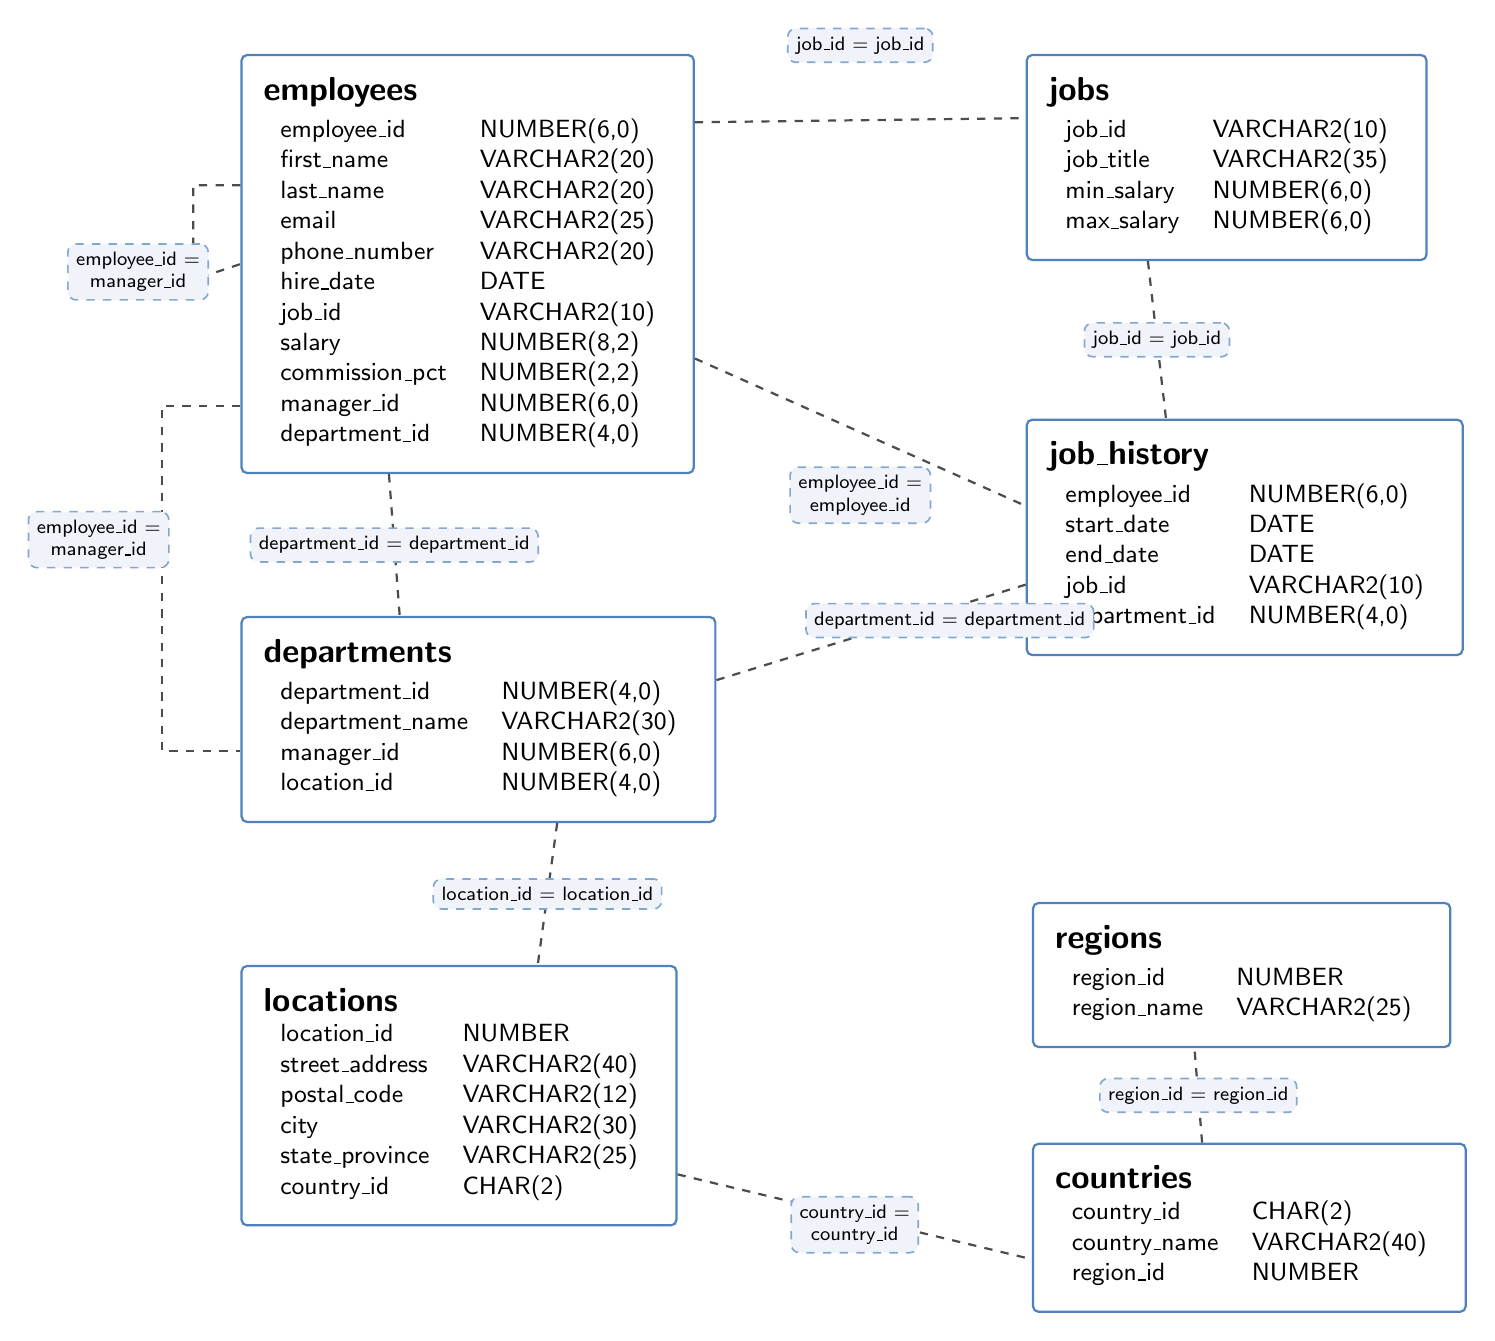
\begin{tikzpicture}[
        >=Stealth,
        line width=0.6pt,
        % Style for the table containers
        table_box/.style={
            draw=borderblue,
            fill=white,
            rounded corners=2pt,
            thick,
            inner sep=8pt,
            font=\sffamily\small,
            align=left
        },
        % Style for the relationship join condition labels
        join_label/.style={
            draw=borderblue!70,
            dashed,
            fill=labelbg,
            rounded corners=3pt,
            font=\sffamily\scriptsize,
            inner sep=3pt,
            align=center
        },
        % Relationship line style
        rel_line/.style={
            draw=black!70,
            dashed,
            thick
        }
    ]

    % ==========================================
    % 1. TABLE DEFINITIONS
    % ==========================================

    % EMPLOYEES
    \node (employees) [table_box] {
        {\large\textbf{employees}}\\[0.6ex]
        \begin{tabular}{ll}
            employee\_id     & NUMBER(6,0) \\
            first\_name      & VARCHAR2(20) \\
            last\_name       & VARCHAR2(20) \\
            email            & VARCHAR2(25) \\
            phone\_number    & VARCHAR2(20) \\
            hire\_date       & DATE \\
            job\_id          & VARCHAR2(10) \\
            salary           & NUMBER(8,2) \\
            commission\_pct  & NUMBER(2,2) \\
            manager\_id      & NUMBER(6,0) \\
            department\_id    & NUMBER(4,0)
        \end{tabular}
    };

    % DEPARTMENTS (Below Employees)
    \node (departments) [table_box, below=1.8cm of employees.south west, anchor=north west] {
        {\large\textbf{departments}}\\[0.6ex]
        \begin{tabular}{ll}
            department\_id   & NUMBER(4,0) \\
            department\_name & VARCHAR2(30) \\
            manager\_id      & NUMBER(6,0) \\
            location\_id     & NUMBER(4,0)
        \end{tabular}
    };

    % LOCATIONS (Below Departments)
    \node (locations) [table_box, below=1.8cm of departments.south west, anchor=north west] {
        {\large\textbf{locations}}\\[0.6ex]
        \begin{tabular}{ll}
            location\_id     & NUMBER \\
            street\_address  & VARCHAR2(40) \\
            postal\_code     & VARCHAR2(12) \\
            city            & VARCHAR2(30) \\
            state\_province  & VARCHAR2(25) \\
            country\_id      & CHAR(2)
        \end{tabular}
    };

    % JOBS (Top Right)
    \node (jobs) [table_box, right=4.2cm of employees.north east, anchor=north west] {
        {\large\textbf{jobs}}\\[0.6ex]
        \begin{tabular}{ll}
            job\_id          & VARCHAR2(10) \\
            job\_title       & VARCHAR2(35) \\
            min\_salary      & NUMBER(6,0) \\
            max\_salary      & NUMBER(6,0)
        \end{tabular}
    };

    % JOB_HISTORY (Middle Right)
    \node (job_history) [table_box, below=2.0cm of jobs.south west, anchor=north west] {
        {\large\textbf{job\_history}}\\[0.6ex]
        \begin{tabular}{ll}
            employee\_id     & NUMBER(6,0) \\
            start\_date      & DATE \\
            end\_date        & DATE \\
            job\_id          & VARCHAR2(10) \\
            department\_id    & NUMBER(4,0)
        \end{tabular}
    };

    % REGIONS (Bottom Right - Top)
    \node (regions) [table_box, right=4.5cm of locations.north east, anchor=north west, yshift=0.8cm] {
        {\large\textbf{regions}}\\[0.6ex]
        \begin{tabular}{ll}
            region\_id       & NUMBER \\
            region\_name     & VARCHAR2(25)
        \end{tabular}
    };

    % COUNTRIES (Bottom Right - Bottom)
    \node (countries) [table_box, below=1.2cm of regions.south west, anchor=north west] {
        {\large\textbf{countries}}\\[0.6ex]
        \begin{tabular}{ll}
            country\_id      & CHAR(2) \\
            country\_name    & VARCHAR2(40) \\
            region\_id       & NUMBER
        \end{tabular}
    };


    % ==========================================
    % 2. RELATIONSHIP LINES AND LABELS
    % ==========================================

    % --- Left side self-loop: employees (manager_id to employee_id) ---
    \draw [rel_line] (employees.west) ++(0, 1.0) -- ++(-0.6, 0) -- ++(0, -1.2) -- (employees.west);
    \node at ($(employees.west) +(-1.3, -0.1)$) [join_label] {employee\_id =\\ manager\_id};

    % --- Left side outer line: employees to departments (manager_id) ---
    \draw [rel_line] (employees.west) ++(0, -1.8) -- ++(-1.0, 0) |- ($(departments.west) + (0, -0.4)$);
    \node at ($(employees.west) +(-1.8, -3.5)$) [join_label] {employee\_id =\\ manager\_id};

    % --- Inner connection: employees to departments (department_id) ---
    \draw [rel_line] (employees.south) ++(-1.0, 0) -- ($(departments.north) + (-1.0, 0)$);
    \node at ($(employees.south) !0.5! (departments.north) + (-1.0, 0)$) [join_label] {department\_id = department\_id};

    % --- Top Horizontal: employees to jobs ---
    \draw [rel_line] (employees.east) ++(0, 1.8) -- ($(jobs.west) + (0, 0.5)$);
    \node at ($(employees.east) !0.5! (jobs.west) + (0, 2.1)$) [join_label] {job\_id = job\_id};

    % --- Vertical: jobs to job_history ---
    \draw [rel_line] (jobs.south) ++(-1.0, 0) -- ($(job_history.north) + (-1.0, 0)$);
    \node at ($(jobs.south) !0.5! (job_history.north) + (-1.0, 0)$) [join_label] {job\_id = job\_id};

    % --- Middle Horizontal: employees to job_history ---
    \draw [rel_line] (employees.east) ++(0, -1.2) -- ($(job_history.west) + (0, 0.4)$);
    \node at ($(employees.east) !0.5! (job_history.west) + (0, -1.2)$) [join_label] {employee\_id =\\ employee\_id};

    % --- Lower Middle Horizontal: departments to job_history ---
    \draw [rel_line] (departments.east) ++(0, 0.5) -- ($(job_history.west) + (0, -0.6)$);
    \node at ($(departments.east) !0.5! (job_history.west) + (1.0, 0.1)$) [join_label] {department\_id = department\_id};

    % --- Lower Vertical: departments to locations ---
    \draw [rel_line] (departments.south) ++(1.0, 0) -- ($(locations.north) + (1.0, 0)$);
    \node at ($(departments.south) !0.5! (locations.north) + (1.0, 0)$) [join_label] {location\_id = location\_id};

    % --- Bottom Horizontal: locations to countries ---
    \draw [rel_line] (locations.east) ++(0, -1.0) -- ($(countries.west) + (0, -0.4)$);
    \node at ($(locations.east) !0.5! (countries.west) + (0, -0.8)$) [join_label] {country\_id =\\ country\_id};

    % --- Bottom Right Vertical: countries to regions ---
    \draw [rel_line] (countries.north) ++(-0.6, 0) -- ($(regions.south) + (-0.6, 0)$);
    \node at ($(countries.north) !0.5! (regions.south) + (-0.6, 0)$) [join_label] {region\_id = region\_id};

    \end{tikzpicture}
\end{center}

\mk{10} \yr{CSE 215 | L-2/T-2 | 2018--19}

\end{enumerate}


%% ══════════════════════════════════════════════════════════════════════
%%  PART III — NORMALIZATION
%% ══════════════════════════════════════════════════════════════════════
\secdivider{Part III}{Normalization}{cC}{cC}

%% ── S4: Normalization ─────────────────────────────────────────────────
\section{S4 --- Normalization}
\label{sec:S4}
\markboth{S4 --- Normalization}{}

%%──────────────────────────────────────────────────────────────────────
\subtopic{cC}{Functional Dependencies}
\label{sub:s4-fd}

\begin{enumerate}

%% Q1
\item Consider a relation with schema $R(A, B, C, D)$ and FDs: $AB \to C$, $C \to D$, and $D \to A$. What are the non-trivial FDs that follow from the given FDs?
\mk{8} \yr{CSE 215 | L-3/T-1 | 2010--11}

%% Q2
\item Consider a relation with schema $R(A, B, C, D)$ and FDs: $AB \to C$, $AD \to B$, $B \to D$. Find all non-trivial FDs that follow from the given FDs.
\mk{10} \yr{CSE 303 | L-3/T-1 | 2011--12}

%% Q3 — 2015-16
\item Consider a relation $R(A, B, C, D)$ and FDs: $AB \to C$, $BC \to D$, $CD \to A$, and $AD \to B$.
\begin{enumerate}
  \item What are all nontrivial FDs that follow from the given FDs? (Restrict yourself to FDs with single attributes on the right side.)
  \item What are all the keys of $R$?
  \item What are all the superkeys for $R$ that are not keys?
\end{enumerate}
\mk{12} \yr{CSE 303 | L-3/T-1 | 2015--16}

%% Q4 — 2016-17 canonical cover
\item Given a set $F$ of functional dependencies on $R(A, B, C)$:
\[A \to BC,\quad B \to C,\quad A \to B,\quad AB \to C\]
\begin{enumerate}
  \item Compute the canonical cover for $F$.
  \item Decompose $R$ into $R_1$ and $R_2$ such that the decomposition is lossless. What are the normal forms of the decomposed relations?
\end{enumerate}
\mk{9} \yr{CSE 303 | L-3/T-1 | 2016--17}

%% Q5 — 2016-17 attribute closure
\item Given a set $F$ of functional dependencies on $r_1(A, B, C, G, H, I)$:
\[A \to B,\quad A \to C,\quad CG \to H,\quad CG \to I,\quad B \to H\]
Compute the attribute closure $(AG)^+$ and show that $AG$ is a candidate key of $r_1$.
\mk{6} \yr{CSE 303 | L-3/T-1 | 2016--17}

%% Q6 — 2017-18 closure of {A,B}
\item Write the steps to compute the closure of a set of attributes with respect to a set of functional dependencies (FD). Consider a relation with attributes $A, B, C, D, E, F$ and the FDs:
\[AB \to C,\quad BC \to AD,\quad D \to E,\quad CF \to B\]
Find the closure of $\{A, B\}$, that is $\{A,B\}^+$.
\mk{10} \yr{CSE 215 | L-2/T-2 | 2017--18}

%% Q7 — 2019-20 six closure rules with examples
\item Write down the six rules with examples to find out the closure of a set of functional dependencies.
\mk{5} \yr{CSE 215 | L-2/T-2 | 2019--20}

%% Q8 — 2020-21 minimal FDs from table (FirstName, LastName, FullName, FullAddress, ZipCode)
\item Consider the following table:

\medskip
\begin{center}
\small
\begin{tabular}{lllllll}
\toprule
\textbf{FirstName} & \textbf{FirstInitial} & \textbf{LastName} & \textbf{LastInitial} & \textbf{FullName} & \textbf{FullAddress} & \textbf{ZipCode}\\
\midrule
Alice & A & Levy  & L & Alice Levy  & 45h St, Seattle, 98185 & 98185\\
Bob   & B & Levy  & L & Bob Levy    & 45h St, Seattle, 98185 & 98185\\
Alice & A & Davis & D & Alice Davis & Oak Ave, Seattle, 98185 & 98185\\
Carol & C & Davis & D & Carol Davis & Sunnyvale, 94085 & 94085\\
Carol & C & Louis & L & Carol Louis & Oak Ave, Seattle, 98185 & 98185\\
\bottomrule
\end{tabular}
\end{center}
\begin{enumerate}
\item Find all functional dependencies that hold on this table. You only need to write a minimal set of functional dependencies that logically imply all others.

\item Using the functional dependencies identified , decompose the relation into BCNF. Show your work and the final normalized schema including all keys.
\end{enumerate}
\mk{20} \yr{CSE 215 | L-2/T-2 | 2020--21}


%% Q9 — 2020-21 FDs for R(A,B,C,D): AB->C, C->D, D->A — nontrivial FDs
\item Consider a relation with schema $R(A, B, C, D)$ and FDs: $AB \to C$, $C \to D$, and $D \to A$.
\begin{enumerate}
  \item What are all the nontrivial FDs that follow from the given FDs? Restrict yourself to FDs with single attributes on the right sides.
  \item What are all the keys of $R$?
  \item What are all the superkeys that are not keys?
\end{enumerate}
 \mk{15} \yr{CSE 215 | L-2/T-2 | 2020--21}

%% Q10 — 2021-22 FDs for R(A,B,C,D,E): A->B, B->C, C->D, D->A
\item Consider a relation with schema $R(A, B, C, D, E)$ and FDs: $A \to B$, $B \to C$, $C \to D$, and $D \to A$.
\begin{enumerate}
  \item What are all the nontrivial FDs that follow from the given FDs? Restrict yourself to FDs with single attributes on the right sides.
  \item What are all the keys of $R$?
  \item What are all the super-keys that are not keys?
\end{enumerate}
\mk{10} \yr{CSE 215 | L-2/T-2 | 2021--22}

%% Q11 — 2024-25 FD closure and key testing: R(A,B,C,D,E), FDs A->C, BE->D, CD->A, BC->E, AD->B
\item Consider a relation with schema $R(A,B,C,D,E)$ and functional dependencies: $A \to C$, $BE \to D$, $CD \to A$, $BC \to E$, and $AD \to B$.
\begin{enumerate}
  \item Determine whether the following functional dependencies follow from the given FDs: $BC \to AD$,\quad $AC \to BD$.
  \item Determine whether the following are keys of the given relation: $\{A,B\}$,\quad $\{A,E\}$.
\end{enumerate}
\mk{10} \yr{CSE 215 | L-2/T-1 | 2024--25}

\end{enumerate}

%%──────────────────────────────────────────────────────────────────────
\subtopic{cC}{Normal Forms (BCNF, 3NF, 4NF)}
\label{sub:s4-nf}

\begin{enumerate}

%% Q1
\item Define BCNF, 3NF, and 4NF. Describe relationships among these normal forms.
\mk{17} \yr{CSE 215 | L-3/T-1 | 2010--11}

%% Q2
\item Describe the BCNF decomposition algorithm.
\mk{10} \yr{CSE 215 | L-3/T-1 | 2010--11}

%% Q3
\item The following schema has been designed for an address book application:
\[R(SSN,\ Name,\ PhoneType,\ PhoneNumber)\]
A person can have different types of phone numbers (e.g.\ Mobile, Home or Office). The following set $F$ of functional dependencies hold on $R$:
\[SSN \to Name\]
\[SSN,\;PhoneType \to PhoneNumber\]
\[SSN,\;PhoneType \to Name\]
\[PhoneNumber \to SSN,\;Name,\;PhoneType\]
\begin{enumerate}
  \item What are the keys for $R$?
  \item Is $R$ in BCNF? Why or why not?
  \item Can you remove any dependency without violating equivalency of $F$?
  \item Decompose $R$ into BCNF (if it is not already in BCNF).
\end{enumerate}
\mk{15} \yr{CSE 303 | L-3/T-1 | 2011--12}

%% Q4
\item Suppose that we have a schema $R = (A, B, C, D)$ with functional dependencies:
\[B \to C \qquad D \to A\]
List the keys of $R$. Is $R$ in BCNF? If not, convert $R$ to BCNF.
\mk{15} \yr{CSE 303 | L-3/T-1 | 2012--13}

%% Q5 — 2015-16
\item Prove that any two-attribute relation is in BCNF.
\mk{7} \yr{CSE 303 | L-3/T-1 | 2015--16}

%% Q6 — 2015-16
\item For the relation schema $R(A, B, C, D, E)$ with FDs $AB \to C$, $DE \to C$, and $B \to D$:
\begin{enumerate}
  \item Indicate all the BCNF violations.
  \item Decompose the relations, as necessary, into a collection of relations that are in BCNF.
\end{enumerate}
\mk{10} \yr{CSE 303 | L-3/T-1 | 2015--16}

%% Q7 — 2015-16
\item Suppose $R$ is a relation with attributes $A_1, A_2, \ldots, A_n$. As a function of $n$, find how many superkeys $R$ has if the only keys are $\{A_1\}$ and $\{A_2, A_3\}$.
\mk{6} \yr{CSE 303 | L-3/T-1 | 2015--16}

%% Q8 — 2014-15
\item Show an example where a table is in 3NF, but not in BCNF. Then modify the design to satisfy BCNF.
\mk{10} \yr{CSE 303 | L-3/T-1 | 2014--15}

\variant{2013--14: ``Show an example where a table is in 3NF, but not in BCNF.'' \mk{5}}

%% Q9 — 2017-18 Address book BCNF (same as 2011-12 — mark as variant)
\item The following schema has been designed for an address book application:
\[R(\underline{SSN},\ Name,\ PhoneType,\ PhoneNumber)\]
The following FDs hold: $SSN \to Name$;\; $SSN, PhoneType \to PhoneNumber$;\; $SSN, PhoneType \to Name$;\; $PhoneNumber \to SSN, Name, PhoneType$.
\begin{enumerate}
  \item What are the keys for $R$?
  \item Is $R$ in BCNF? Why or why not?
  \item Decompose $R$ into BCNF (if not already in BCNF).
\end{enumerate}
\mk{15} \yr{CSE 215 | L-2/T-2 | 2017--18}

\variant{2011--12: same question with additional subpart (iii) ``Can you remove any dependency without violating equivalency of $F$?''}

%% Q10 — 2017-18 3NF but not BCNF + MVD
\item Give an example of a relation which is in 3NF but not in BCNF. Define Multivalued Dependency.
\mk{10} \yr{CSE 215 | L-2/T-2 | 2017--18}

%% Q11 — 2018-19 3NF agreement question
\item ``A table in 3NF may fail to meet the criteria of BCNF'' --- do you agree? Show an appropriate example to validate your claim.
\mk{10} \yr{CSE 215 | L-2/T-2 | 2018--19}

%% Q12 — 2019-20 BCNF and 3NF definition + BCNF decomposition
\item What do you know about BCNF and 3NF? What is the major difference between them? Let $R$ be a schema that is not in BCNF and $\alpha \to \beta$ be the functional dependency that causes a violation of BCNF. How can $R$ be decomposed such that $R$ will be in BCNF?
\mk{10} \yr{CSE 215 | L-2/T-2 | 2019--20}

%% Q13 — 2019-20 lossless decomposition check: R=(A,B,C,D,E) -> (A,B,C) and (A,D,E)
\item Suppose that we decompose the schema $R = (A, B, C, D, E)$ into $(A, B, C)$ and $(A, D, E)$. Show whether this decomposition is a lossless decomposition if the following set $F$ of functional dependencies holds:
\[A \to BC,\quad CD \to E,\quad B \to D,\quad E \to A\]
\mk{10} \yr{CSE 215 | L-2/T-2 | 2019--20}

%% Q14 — 2020-21 BCNF decomposition of table (FirstName, LastName, FullName, FullAddress, ZipCode)

%% Q15 — 2021-22 BCNF decomposition of R(A,B,C,D,E) with FDs AB->C, DE->C, B->D
\item Consider a relation with schema $R(A, B, C, D, E)$ and FDs: $AB \to C$, $DE \to C$, and $B \to D$. Decompose the relations, as necessary, into collections of relations that are in BCNF. Show your work and the final normalized schema including all keys.
\mk{20} \yr{CSE 215 | L-2/T-2 | 2021--22}



%% Q17 — 2023-24 3NF but not BCNF example + modify to BCNF
\item Discuss an example where a table is in 3NF but not in BCNF. Then, modify the design to satisfy BCNF.
\mk{9} \yr{CSE 215 | L-2/T-1 | 2023--24}

%% Q18 — 2023-24 normalize invoice table to 3NF (INV_NUM, PROD_NUM, etc.)
\item Why is the normalization technique used in database design? Normalize the following table by drawing a dependency diagram and identifying all dependencies to derive up to 3NF. Show the schema in 3NF.

\medskip
\begin{center}
\small
\begin{tabular}{llllll}
\toprule
\textbf{Attribute} & \textbf{Sample 1} & \textbf{Sample 2} & \textbf{Sample 3} & \textbf{Sample 4} & \textbf{Sample 5}\\
\midrule
INV\_NUM    & 211347 & 211347 & 211347 & 211348 & 211349\\
PROD\_NUM   & AA-E3422QW & QD-300932X & RU-995748G & AA-E3422QW & GH-778345P\\
SALE\_DATE  & 15-Jan-2010 & 15-Jan-2010 & 15-Jan-2010 & 15-Jan-2010 & 16-Jan-2010\\
PROD\_LABEL & Rotary sander & 0.25-in.\ drill bit & Band saw & Rotary sander & Power drill \\
VEND\_CODE  & 211 & 211 & 309 & 211 & 157\\
VEND\_NAME  & NeverFail Inc. & NeverFail Inc. & BeGood Inc. & NeverFail Inc. & ToughGo. Inc\\
QUANT\_SOLD & 1 & 8 & 1 & 2 & 1\\
PROD\_PRICE & \$49.95 & \$3.45 & \$39.99 & \$49.95 & \$87.75\\
\bottomrule
\end{tabular}
\end{center}
\mk{15} \yr{CSE 215 | L-2/T-1 | 2023--24}

%% Q19 — 2024-25 superkey count as function of n
\item Suppose $R$ is a relation with attributes $A_1, A_2, \ldots, A_n$. As a function of $n$, determine how many superkeys $R$ has for each of the following cases:
\begin{enumerate}
  \item The only key is $A_1$.
  \item The only keys are $\{A_1, A_2\}$ and $\{A_1, A_3\}$.
\end{enumerate}
\mk{8} \yr{CSE 215 | L-2/T-1 | 2024--25}

%% Q20 — 2024-25 BCNF decomposition of R(A,B,C,D,E) with ABE->C, BC->D, BD->E, DE->A
\item For a relation schema $R(A,B,C,D,E)$, consider the following set of functional dependencies: $ABE \to C$, $BC \to D$, $BD \to E$, $DE \to A$. Decompose the relation into BCNF. Show the final schemas and the projected functional dependencies for each schema after decomposition. Is your final decomposition dependency-preserving? Justify your answer.
\mk{16} \yr{CSE 215 | L-2/T-1 | 2024--25}

\end{enumerate}

%%──────────────────────────────────────────────────────────────────────
\subtopic{cC}{Anomalies \& Normalization}
\label{sub:s4-anomaly}

\begin{enumerate}

%% Q1
\item What are redundancy, deletion and update anomalies?
\mk{10} \yr{CSE 303 | L-3/T-1 | 2011--12}

%% Q2
\item What are the three anomalies in relational database schemas? Discuss them.
\mk{10} \yr{CSE 303 | L-3/T-1 | 2012--13}

\variant{2013--14: same question \mk{10}}

%% Q3 — 2014-15 booking table normalization
\item Normalize the following booking table up to 3NF by drawing a dependency diagram and identifying all dependencies. Show the resulting 3NF schema.

\medskip
\begin{center}
\small
\begin{tabular}{lllllllll}
\toprule
\textbf{Date} & \textbf{Time} & \textbf{Customer} & \textbf{Contact} & \textbf{Event} & \textbf{Person} & \textbf{Total} & \textbf{Price}\\
\midrule
12 Aug, 10 & 12.30 PM & Maria Indrawan & 04222223333 & Lunch & Dora Smith & 6 & 60\\
12 Aug, 10 & 12.30 PM & John Smith & 04113333333 & Master Class & Simon Becket & 1 & 120\\
12 Aug, 10 & 7.00 PM & Mary Joe & 95671290 & Dinner & Linda Dee & 2 & 150\\
13 Aug, 10 & 12.30 PM & Lindsay Smith & 99031001 & Lunch & Dora Smith & 4 & 60\\
13 Aug, 10 & 12.30 PM & Sunshine Dee & 99021900 & Lunch & Dora Smith & 2 & 60\\
\bottomrule
\end{tabular}
\end{center}
\mk{13} \yr{CSE 303 | L-3/T-1 | 2014--15}

%% Q4 — 2013-14 invoice table normalization
\item Normalize the following invoice table up to 3NF by drawing a dependency diagram and identifying all dependencies. Show the resulting 3NF schema.

\medskip
\begin{center}
\small
\begin{tabular}{lllllllll}
\toprule
\textbf{INV\_NUM} & \textbf{PROD\_NUM} & \textbf{SALE\_DATE} & \textbf{PROD\_LABEL} & \textbf{VEND\_CODE} & \textbf{VEND\_NAME} & \textbf{QTY} & \textbf{PRICE}\\
\midrule
211347 & AA-E3422QW & 15-Jan-2010 & Rotary Sander & 211 & NeverFail, Inc & 1 & \$49.95\\
211347 & QD-300932X & 15-Jan-2010 & 0.25-in drill bit & 211 & NeverFail, Inc & 8 & \$3.45\\
211347 & RU-995748G & 15-Jan-2010 & Band Saw & 309 & BeGood, Inc. & 1 & \$39.99\\
211348 & AA-E3422QW & 15-Jan-2010 & Rotary Sander & 211 & NeverFail, Inc. & 2 & \$49.95\\
211349 & GH-7781 & 16-Jan-2010 & Power drill & 157 & ToughGood & 1 & \$87.75\\
\bottomrule
\end{tabular}
\end{center}
\mk{15} \yr{CSE 303 | L-3/T-1 | 2013--14}

%% Q5 — 2018-19 StaffPropertyInspection 2NF normalization
\item Suppose we are generating a \texttt{StaffPropertyInspection} table to include property inspection
by staff members. When the staffs are required to undertake the inspections, they are
allocated a company car for use on the day of the inspections. However, a car may be allocated
to several staff members on the same day at different time slots. A member of staff
may inspect several properties on a given date, but a property is only inspected once by a
single staff member on a given date.
Normalize the \texttt{StaffPropertyInspection} table (Figure 2) up to 2NF. Show only the following steps:\\
Hint: you have to perform and only show the results of the following steps:
\begin{enumerate}
  \item Find all the candidate keys.
  \item Determine the primary key.
  \item Find all the functional dependencies.
  \item Get the first normal form (1NF).
  \item Get the second normal form (2NF).
\end{enumerate}

  \noindent \textbf{StaffPropertyInspection} \\[1ex]
\begin{center}
\renewcommand{\arraystretch}{1.5} % Adds a little padding to the rows
\begin{tabular}{|l|l|l|p{3.5cm}|p{4cm}|l|l|l|}
\hline
\textbf{propertyNo} & \textbf{iDate} & \textbf{iTime} & \textbf{pAddress} & \textbf{comments} & \textbf{staffNo} & \textbf{sName} & \textbf{carReg} \\
\hline \hline
PG4  & 18-Oct-00 & 10.00 & 6 Lawrence St, Glasgow & Need to replace crockery   & SG37 & Ann Beech  & M231 JGR \\ \hline
PG4  & 22-Apr-01 & 09.00 & 6 Lawrence St, Glasgow & In good order              & SG14 & David Ford & M533 HDR \\ \hline
PG4  & 1-Oct-01  & 12.00 & 6 Lawrence St, Glasgow & Damp rot in bathroom       & SG14 & David Ford & N721 HFR \\ \hline
PG16 & 22-Apr-01 & 13.00 & 5 Novar Dr, Glasgow    & Replace living room carpet & SG14 & David Ford & M533 HDR \\ \hline
PG16 & 24-Oct-01 & 14.00 & 5 Novar Dr, Glasgow    & Good condition             & SG37 & Ann Beech  & N721 HFR \\ 
\hline
\end{tabular}
\end{center}
\mk{10} \yr{CSE 215 | L-2/T-2 | 2018--19}

\end{enumerate}


%% ══════════════════════════════════════════════════════════════════════
%%  PART IV — STORAGE, INDEXING & QUERY PROCESSING
%% ══════════════════════════════════════════════════════════════════════
\secdivider{Part IV}{Storage, Indexing \& Query Processing}{cD}{cD}

%% ── S5: Storage and Indexing ──────────────────────────────────────────
\section{S5 --- Storage and Indexing}
\label{sec:S5}
\markboth{S5 --- Storage and Indexing}{}

%%──────────────────────────────────────────────────────────────────────
\subtopic{cD}{Data Storage Architecture \& RAID}
\label{sub:s5-storage}

\begin{enumerate}

%% Q1
\item Explain block level striping with an example of storing $1, 2, \ldots, n$ logical blocks into a disk subsystem consisting of 8 disks.
\mk{5} \yr{CSE 215 | L-3/T-1 | 2010--11}

%% Q2
\item What are the different types of disk failures? How does a DBMS handle a disk crash?
\mk{8} \yr{CSE 303 | L-3/T-1 | 2011--12}

%% Q3
\item Find a RAID level 6 scheme with ten disks, such that it is possible to recover from the failure of any three disks simultaneously. You should use as many data disks as you can.
\mk{15} \yr{CSE 303 | L-3/T-1 | 2011--12}

\variant{CSE 215 | L-3/T-1 | 2012--13}

%% Q4
\item What are the differences between RAID levels 1, 4, 5 and 6?
\mk{12} \yr{CSE 303 | L-3/T-1 | 2011--12}

%% Q5 — 2014-15
\item Discuss the applications where you will use RAID level 1 and RAID level 5.
\mk{5} \yr{CSE 303 | L-3/T-1 | 2014--15}

%% Q6 — 2013-14 RAID with 15 disks
\item Find a RAID level 6 scheme with 15 disks, four of which are redundant.
\mk{15} \yr{CSE 303 | L-3/T-1 | 2013--14}

%% Q7 — 2015-16 file deletion methods
\item Figure 3 shows a fixed-length record file structure for a \texttt{Customer} relation with fields: record\#, CustomerID, Name, Street, City, Balance (records C0001--C0010). Show the file structure after deletion of records with customer IDs C004 and C007 for different file deletion methods. Compare the advantages and disadvantages among the different deletion methods.

\medskip
\begin{center}
\small
\begin{tabular}{llllll}
\toprule
\textbf{Record} & \textbf{CustID} & \textbf{Name} & \textbf{Street} & \textbf{City} & \textbf{Balance}\\
\midrule
0 & C0001 & N1 & North & Dhaka & 1000\\
1 & C0002 & N2 & North & Dhaka & 2000\\
2 & C0003 & N3 & North & Dhaka & 3000\\
3 & C0004 & N4 & North & Dhaka & 4000\\
4 & C0005 & N5 & North & Dhaka & 5000\\
5 & C0006 & N6 & South & Dhaka & 6000\\
6 & C0007 & N7 & South & Dhaka & 7000\\
7 & C0008 & N8 & South & Dhaka & 8000\\
8 & C0009 & N9 & South & Dhaka & 9000\\
9 & C0010 & N10 & South & Dhaka & 10000\\
\bottomrule
\end{tabular}
\end{center}
\mk{15} \yr{CSE 303 | L-3/T-1 | 2015--16}

%% Q8 — 2014-15 fixed-length record deletion (student relation)
\item A file containing fixed-length records of a \texttt{student} relation (attributes: student\_id, name, department\_code, level, term) is given. Show the file structures after deletion of record 3 for the following cases and give comparative advantages/disadvantages:
\begin{enumerate}
  \item Move record 4 to the space occupied by record 3, record 5 to record 4, and so on.
  \item Move record 8 to the space occupied by record 3.
  \item Mark record 3 as deleted and move no records. Use a header and record pointer.
\end{enumerate}
\mk{15} \yr{CSE 303 | L-3/T-1 | 2014--15}

%% Q9 — 2014-15 multitable clustering
\item The relation \texttt{student(student\_id, name, dept\_code, level, term)} and \texttt{department(dept\_code, location, floors, type)} are given (dept\_code is PK of department and FK in student).
\begin{enumerate}
  \item Show the multitable clustering file structure for the given relations. Explain why executing \texttt{SELECT * FROM department} is more expensive in this structure.
  \item Show the multitable clustering file structure with pointer chain. How is the query in (i) executed faster in this structure?
\end{enumerate}

\begin{center}
  \renewcommand{\arraystretch}{1.3} % Slightly expands row height for readability
    \begin{tabular}{l |c|c|c|c|c|}
        \cline{2-6}
        Record 0 & 1205001 & N11 & CSE & 3 & 1 \\
        \cline{2-6}
        Record 1 & 1205004 & N12 & CSE & 3 & 1 \\
        \cline{2-6}
        Record 2 & 1205007 & N13 & CSE & 3 & 1 \\
        \cline{2-6}
        Record 3 & 1205010 & N14 & CSE & 3 & 1 \\
        \cline{2-6}
        Record 4 & 1205013 & N15 & CSE & 3 & 1 \\
        \cline{2-6}
        Record 5 & 1205016 & N16 & CSE & 3 & 1 \\
        \cline{2-6}
        Record 6 & 1204001 & N21 & EEE & 3 & 1 \\
        \cline{2-6}
        Record 7 & 1204002 & N22 & EEE & 3 & 1 \\
        \cline{2-6}
        Record 8 & 1204003 & N23 & EEE & 3 & 1 \\
        \cline{2-6}
    \end{tabular}
    
    \vspace{0.4cm}
    \textbf{Figure 1:} File containing records of relation \textit{student}(\underline{\textit{student id}}, \textit{name}, \textit{department code}, \textit{level}, \textit{term})

\vspace{1cm}

% ==========================================
% FIGURE 2: Department Relation Table
% ==========================================
    \renewcommand{\arraystretch}{1.3}
    \begin{tabular}{|c|c|c|c|}
        \hline
        CSE & ECE BUILDING & 12 & A \\
        \hline
        EEE & ME BUILDING & 6 & B \\
        \hline
    \end{tabular}
    
    \vspace{0.4cm}
    \textbf{Figure 2:} File containing records of relation \textit{department}(\underline{\textit{department code}}, \textit{location}, \textit{floors}, \textit{type})
\end{center}
\mk{15} \yr{CSE 303 | L-3/T-1 | 2014--15}

%% Q10 — 2013-14 disk performance
\item What are the different ways to improve the performance of a disk-based system?
\mk{5} \yr{CSE 303 | L-3/T-1 | 2013--14}

%% Q11 — 2013-14 Elevator algorithm
\item Write down the pros and cons of an Elevator algorithm.
\mk{5} \yr{CSE 303 | L-3/T-1 | 2013--14}

%% Q12 — 2013-14 Megatron 747 disk
\item The Megatron 747 disk has the following characteristics:
\begin{itemize}[leftmargin=1.5em,itemsep=1pt]
  \item 4 Platters providing 8 surfaces
  \item 8192 tracks per surface, 256 sectors per track, 512 bytes per sector
  \item Disk rotates at 3840 rpm (one rotation every 15.6 ms)
  \item Average seek time: 6.5 ms
  \item Transfer rate: 10 MB/s
\end{itemize}
\begin{enumerate}
  \item What is the capacity of a single track and what is the size of the entire disk?
  \item What is the average read time of 4096 bytes of data?
\end{enumerate}
  \mk{7} \yr{CSE 303 | L-3/T-1 | 2013--14}

%% Q13 — 2016-17 disk latency components
\item What are the components of disk latency?
\mk{2} \yr{CSE 303 | L-3/T-1 | 2016--17}

%% Q14 — 2016-17 Megatron 777 disk
\item The Megatron 777 disk has the following characteristics: ten surfaces with 10,000 tracks each; tracks hold an average of 1000 sectors of 512 bytes each; disk rotates at 10,000 rpm; time to move head $n$ tracks is $1 + 0.001n$ milliseconds. Answer:
\begin{enumerate}
  \item What is the capacity of the disk?
  \item What is the maximum seek time?
  \item What is the average rotational latency?
\end{enumerate}
\mk{5} \yr{CSE 303 | L-3/T-1 | 2016--17}

%% Q15 — 2016-17 Elevator algorithm (Megatron 777)
\item Another Megatron 777 disk incurs average rotational latency of 8.3 ms. Moving the head takes 1 ms to start/stop plus 1 ms per 500 cylinders. The disk controller receives the following requests:

\medskip
\begin{center}
\begin{tabular}{ll}
\toprule
\textbf{Cylinder} & \textbf{First Available (ms)}\\
\midrule
1000 & 0\\
3000 & 0\\
7000 & 0\\
2000 & 20\\
8000 & 30\\
5000 & 40\\
\bottomrule
\end{tabular}
\end{center}
Show the finishing time and latency for each request using the elevator algorithm.
  \mk{10} \yr{CSE 303 | L-3/T-1 | 2016--17}

%% Q16 — 2016-17 RAID level 4 update policy
\item In RAID level 4, one redundant disk is used regardless of how many data disks there are. When any block is written, the redundant disk must also be updated. Briefly explain an optimal policy for updating the redundant disk with an example (consider 1 byte of data is written). Explain the logic behind adopting such a policy.
\mk{15} \yr{CSE 303 | L-3/T-1 | 2016--17}

%% Q17 — 2016-17 stable storage
\item What is stable storage? Briefly explain the idea of reading and writing policy in stable storage.
\mk{10} \yr{CSE 303 | L-3/T-1 | 2016--17}

%% Q18 — 2017-18 RAID level 6 with 6 data disks
\item Design a RAID level 6 scheme for six data disks (numbered 1--6) using the minimum number of redundant disks possible. You are not allowed to use any data disk as a redundant disk.
\begin{enumerate}
  \item Describe the recovery process if Disk 1 and Disk 3 fail simultaneously.
  \item Describe the recovery process if Disks 1, 3 and 6 fail simultaneously.
\end{enumerate}
\mk{16} \yr{CSE 215 | L-2/T-2 | 2017--18}

%% Q19 — 2017-18 Average read time Megatron 747
\item Calculate the average time (with explanation) to read one block of data from a Megatron 747 disk (8192 tracks). Given data:

\medskip
\begin{center}
\begin{tabular}{lllll}
\toprule
 & \textbf{Seek (ms)} & \textbf{Rot.\ Latency (ms)} & \textbf{Transfer (ms)} & \textbf{Total (ms)}\\
\midrule
Minimum & 0 & 0 & 0.5 & 0.5\\
Maximum & 17.4 & 15.6 & 0.5 & 33.5\\
\bottomrule
\end{tabular}
\end{center}
  \mk{8} \yr{CSE 215 | L-2/T-2 | 2017--18}

%% Q20 — 2017-18 Elevator algorithm (cylinder requests)
\item Schedule the following cylinder requests using the elevator algorithm. Use data from the Megatron 747 disk question. Assume moving the head requires 1 ms (start/stop) + 1 ms per 500 cylinders; head is initially on the 1st cylinder.

\medskip
\begin{center}
\begin{tabular}{ll}
\toprule
\textbf{Cylinder} & \textbf{Arrival Time (ms)}\\
\midrule
2000 & 0\\
5000 & 10\\
1000 & 15\\
8000 & 25\\
9000 & 35\\
4000 & 50\\
\bottomrule
\end{tabular}
\end{center}
  \mk{9} \yr{CSE 215 | L-2/T-2 | 2017--18}

%% Q21 — 2018-19 RAID level 5 with 4 disks
\item Describe the storage mechanism, data read and update of data blocks for RAID level 5 storage with 4 disks (D0, D1, D2, D3) and a relation with 8 blocks (B0--B7). Describe the full recovery mechanism of all blocks of D1 if disk D1 fails.
\mk{15} \yr{CSE 215 | L-2/T-2 | 2018--19}

%% Q22 — 2018-19 Slotted page structure
\item Given the relational schema:
\begin{center}
\begin{tabular}{l}
\texttt{Student(\underline{id}, name, DOB, cgpa, tot\_cred, house\_no, street, city, remarks, NID)}\\
\texttt{Takes(\underline{id}, \underline{course\_no}, semester, year, grade)}\\
\texttt{Course(\underline{course\_no}, title, credit, pre\_req)}
\end{tabular}
\end{center}
Tuple sizes: Student = 400 bytes, Takes = 100 bytes, Course = 80 bytes. Block size = 8000 bytes. Show the organisation of the slotted page structure after insertion of:
\begin{enumerate}
  \item Two tuples of Student.
  \item Two tuples of Takes.
  \item One tuple of Course.
\end{enumerate}
 \mk{15} \yr{CSE 215 | L-2/T-2 | 2018--19}

%% Q23 — 2019-20 disk access time
\item Explain disk access time and its implication in DBMS.
\mk{5} \yr{CSE 215 | L-2/T-2 | 2019--20}

%% Q24 — 2019-20 block-level vs bit-level striping + RAID 5 with 7 disks
\item Compare between block-level striping and bit-level striping with examples. Show the storage of blocks $B_0, B_1, B_2, \ldots, B_{11}$ of a relation $r$ into a RAID level 5 storage system with 7 disks.
\mk{20} \yr{CSE 215 | L-2/T-2 | 2019--20}

%% Q25 — 2019-20 RAID 5 single disk failure recovery
\item Explain the data recovery mechanism for single disk failure in RAID level 5 with an example.
\mk{10} \yr{CSE 215 | L-2/T-2 | 2019--20}

%% Q26 — 2020-21 fixed-length record storage in blocks
\item A table \texttt{student} has been created as follows:
\begin{lstlisting}
CREATE TABLE STUDENT(
    ID          VARCHAR2(10),
    NAME        VARCHAR2(50),
    CGPA        NUMBER(8),
    ADDRESS     VARCHAR2(932),
    DESCRIPTION VARCHAR2(500)
);
\end{lstlisting}
There are three blocks 1, 2 and 3 and the size of each block is 4000 bytes. Show the storage of 5 sample records of the student relation in these blocks using fixed-length record structure. No record can overlap the block boundary.
 \mk{10} \yr{CSE 215 | L-2/T-2 | 2020--21}

%% Q27 — 2020-21 slotted-page with variable length records + deletion
\item Show and explain the slotted-page structure by inserting two variable length records with size $S_1$ and $S_2$. The block size is 4000 bytes. Show the structure after deletion of the record of size $S_1$.
\mk{15} \yr{CSE 215 | L-2/T-2 | 2020--21}

%% Q28 — 2020-21 multitable clustering (department + instructor)
\item The \texttt{department} and \texttt{instructor} relations are given. Show the multi-table clustering file organization for these relations and explain the types of queries for which this organization will be efficient and the type for which it is inefficient.

\begin{center}
  % First Table (Department)
    \begin{tabular}{|l|l|l|}
        \hline
        \textit{dept\_name} & \textit{building} & \textit{budget} \\
        \hline \hline
        Comp. Sci. & Taylor & 100000 \\
        Physics & Watson & 70000 \\
        \hline
    \end{tabular}
    \hspace{1cm} % Adds horizontal space between the two tables
    % Second Table (Instructor/Employee)
    \begin{tabular}{|l|l|l|l|}
        \hline
        \textit{ID} & \textit{name} & \textit{dept\_name} & \textit{salary} \\
        \hline \hline
        10101 & Srinivasan & Comp. Sci. & 65000 \\
        33456 & Gold & Physics & 87000 \\
        45565 & Katz & Comp. Sci. & 75000 \\
        83821 & Brandt & Comp. Sci. & 92000 \\
        \hline
    \end{tabular}
\end{center}

\mk{10} \yr{CSE 215 | L-2/T-2 | 2020--21}

%% Q29 — 2020-21 RAID 5 and RAID 6 (6 disks, 10 blocks)
\item You have been given 6 disks of 4TB each and a student relation has 10 blocks: $B_0, B_1, \ldots, B_9$. Show the storage of the student relation using:
\begin{enumerate}
  \item RAID level 5 storage system.
  \item RAID level 6 storage system.
  \item Compare RAID level 5 with RAID level 6.
\end{enumerate}
\mk{10} \yr{CSE 215 | L-2/T-2 | 2020--21}

%% Q30 — 2021-22 fixed-length records with free list (insert + delete)
\item A relational database table is stored in a database file using fixed-length records and a free list.
\begin{enumerate}
  \item Show the structure of the file after deleting Record 2 (Mohammad Naim) and inserting a new row (Tamim Iqbal, Batter, 34).
  \item Discuss how the table would be stored in a slotted page structure with a high-level block diagram showing only the records.
\end{enumerate}

\begin{center}
  \renewcommand{\arraystretch}{1.2} % Gives rows slightly more breathing room
\begin{tabular}{|l|l|l|l|l|}
\hline
\textbf{Header} & \textbf{Player Name} & \textbf{Role} & \textbf{Age} & \textbf{Free List}\tikzmark{nodeH} \\ \hline
Record 0 & Shakib Al Hasan & Allrounder & 36 & - \\ \hline
Record 1 & & & & \tikzmark{node1} \\ \hline
Record 2 & Mohammad Naim & Batter & 24 & \\ \hline
Record 3 & Taskin Ahmed & Bowler & 28 & \\ \hline
Record 4 & & & & \tikzmark{node4} \\ \hline
Record 5 & Mushfiqur Rahim & Batter & 36 & \\ \hline
Record 6 & & & & \tikzmark{node6} \\ \hline
Record 7 & Litton Das & Batter & 28 & \\ \hline
Record 8 & Mustafizur Rahman & Bowler & 28 & \\ \hline
\multicolumn{5}{|c|}{\textbf{Figure: 5(c)}} \\ \hline
\end{tabular}

% --- TikZ code to draw the linked list arrows ---
\begin{tikzpicture}[overlay, remember picture, thick, >=stealth]
    % Get the coordinates of the nodes we placed in the table
    \coordinate (H) at (pic cs:nodeH);
    \coordinate (R1) at (pic cs:node1);
    \coordinate (R4) at (pic cs:node4);
    \coordinate (R6) at (pic cs:node6);

    % Draw the linked list arrows outside the table on the right
    % Arrow 1: From Header to Record 1
    \draw[->] ([xshift=10pt, yshift=4pt]H) -- ++(25pt,0) |- ([xshift=10pt, yshift=4pt]R1);
    
    % Arrow 2: From Record 1 to Record 4
    \draw[->] ([xshift=10pt, yshift=-3pt]R1) -- ++(35pt,0) |- ([xshift=10pt, yshift=4pt]R4);
    
    % Arrow 3: From Record 4 to Record 6
    \draw[->] ([xshift=10pt, yshift=-3pt]R4) -- ++(35pt,0) |- ([xshift=10pt, yshift=4pt]R6);
\end{tikzpicture}
\end{center}
\mk{10} \yr{CSE 215 | L-2/T-2 | 2021--22}

%% Q31 — 2021-22 RAID-5 vs RAID-6 differences
\item Briefly describe the differences between RAID-5 and RAID-6.
\mk{5} \yr{CSE 215 | L-2/T-2 | 2021--22}

%% Q32 — 2021-22 disk seek time SCAN vs C-SCAN
\item A Megatron 800 Disk has the following pending disk requests (listed by track number). If the head is currently at track 71 and moving towards the higher track number, calculate average disk seek times for both the SCAN and C-SCAN algorithms.

\medskip
\begin{center}
\begin{tabular}{l}
\toprule
\textbf{Disk Requests}: 21, 98, 12, 80, 85, 10\\
\bottomrule
\end{tabular}
\end{center}
\mk{10} \yr{CSE 215 | L-2/T-2 | 2021--22}

%% Q33 — 2022-23 slotted page structure for BUET course table (varchar + fixed-length)
\item The following table stores information about courses offered by BUET:
\begin{lstlisting}
CREATE TABLE course (
    course_code    CHAR(10) PRIMARY KEY,
    course_title   VARCHAR(255) NOT NULL,
    credit_hours   NUMERIC NOT NULL,
    old_course_code CHAR(10) REFERENCES course(course_code)
);
\end{lstlisting}
Here \texttt{VARCHAR} is variable-length, all other data types are fixed length, size of \texttt{NUMERIC} is 8 bytes, and size of \texttt{CHAR(n)} is $n$ bytes. Draw the structure of the records, and the structure of the page when the records of this table are stored using the Slotted Page Structure.
 \mk{10} \yr{CSE 215 | L-2/T-1 | 2022--23}

%% Q34 — 2024-25 RAID level 4 parity calculation (4 data disks + 1 redundant)
\item Suppose we are using a RAID level 4 scheme with four data disks and one redundant disk, where each block is one byte. Calculate the block of the redundant disk if the corresponding blocks of data disks are: 01010110, 11000000, 00111011, and 11111011.
\mk{10} \yr{CSE 215 | L-2/T-1 | 2024--25}

%% Q35 — 2024-25 multitable clustering file organization
\item What is the purpose of using multiple clustering file organization? Give an example of its usage. Mention the disadvantages of this organization.
\mk{10} \yr{CSE 215 | L-2/T-1 | 2024--25}

\end{enumerate}

%%──────────────────────────────────────────────────────────────────────
\subtopic{cD}{Primary Index}
\label{sub:s5-primary}

\begin{enumerate}

%% Q1
\item Explain the factors by which an indexing technique can be evaluated.
\mk{5} \yr{CSE 215 | L-3/T-1 | 2010--11}

%% Q2 — 2014-15 sparse + secondary index
\item Create the following index structures for the given student relation:
\begin{enumerate}
  \item A sparse index on \texttt{student\_id} for search key values \{1204001, 1205001, 1205010\}.
  \item A secondary index on \texttt{department\_code}.
  \item Delete the record with \texttt{student\_id} = 1205010 and show the resulting index structures.
  \item Insert the record \{1205011, N114, EEE, 3, 1\} and show the resulting index structures.
\end{enumerate}

\begin{center}
  
  \renewcommand{\arraystretch}{1.3} % Slightly expands row height for readability
    \begin{tabular}{l |c|c|c|c|c|}
        \cline{2-6}
        Record 0 & 1205001 & N11 & CSE & 3 & 1 \\
        \cline{2-6}
        Record 1 & 1205004 & N12 & CSE & 3 & 1 \\
        \cline{2-6}
        Record 2 & 1205007 & N13 & CSE & 3 & 1 \\
        \cline{2-6}
        Record 3 & 1205010 & N14 & CSE & 3 & 1 \\
        \cline{2-6}
        Record 4 & 1205013 & N15 & CSE & 3 & 1 \\
        \cline{2-6}
        Record 5 & 1205016 & N16 & CSE & 3 & 1 \\
        \cline{2-6}
        Record 6 & 1204001 & N21 & EEE & 3 & 1 \\
        \cline{2-6}
        Record 7 & 1204002 & N22 & EEE & 3 & 1 \\
        \cline{2-6}
        Record 8 & 1204003 & N23 & EEE & 3 & 1 \\
        \cline{2-6}
    \end{tabular}
    
    \vspace{0.4cm}
    \textbf{Figure 1:} File containing records of relation \textit{student}(\underline{\textit{student id}}, \textit{name}, \textit{department code}, \textit{level}, \textit{term})

\end{center}

\mk{20} \yr{CSE 303 | L-3/T-1 | 2014--15}

%% Q3 — 2017-18 dense vs sparse (dictionary analogy)
\item Consider a dictionary where each page contains only a single word along with its description. If we take the word from each page and form an index based on those words, what type of indexing (Dense/Sparse) would it be? Explain your answer.
\mk{5} \yr{CSE 215 | L-2/T-2 | 2017--18}

%% Q4 — 2018-19 sparse index query execution
\item Explain how the following queries will be executed using the sparse index shown in Figure 1:
\begin{enumerate}
  \item \texttt{SELECT * FROM instructor WHERE id = 22222}
  \item \texttt{SELECT * FROM instructor WHERE id = 99999}
\end{enumerate}
Also explain the deletion of records from 10101 to 22222 from the instructor relation as per the deletion algorithm for a relation with a sparse index.

\begin{center}
      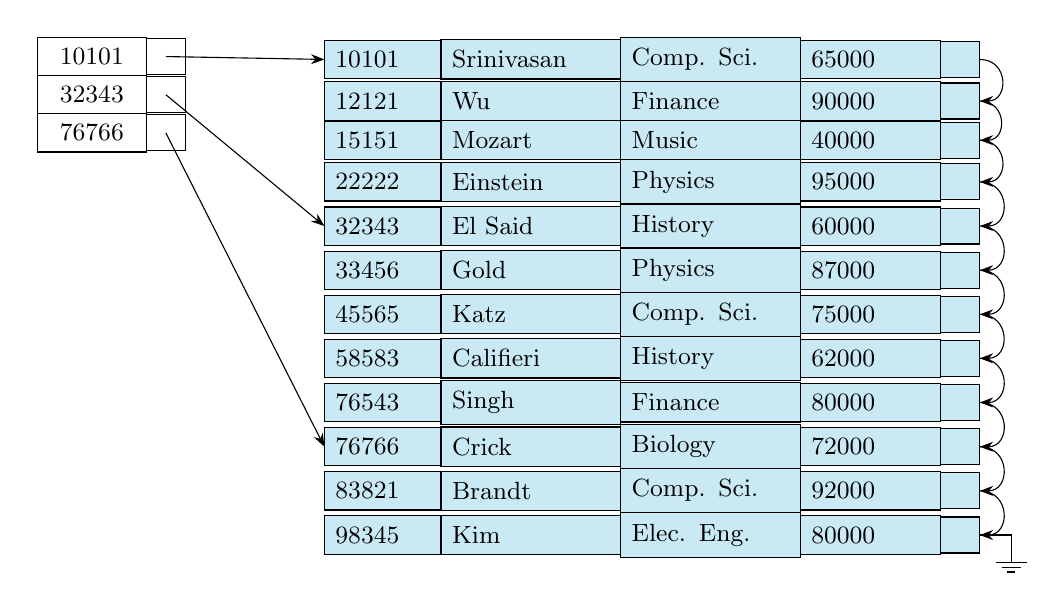
\begin{tikzpicture}[
        >=Stealth,
        % Base style for all cells to ensure borders are drawn
        cell/.style={
            draw, 
            minimum height=1.3em, 
            inner sep=4pt, 
            outer sep=0pt, 
            anchor=center, 
            font=\small
        },
        % Style for the Left Index Table
        index_table/.style={
            matrix of nodes,
            nodes={cell},
            column 1/.style={nodes={text width=1.1cm, align=center}},
            column 2/.style={nodes={minimum width=0.5cm}},
            row sep=-\pgflinewidth,
            column sep=-\pgflinewidth
        },
        % Style for the Right Relation Table
        relation_table/.style={
            matrix of nodes,
            nodes={cell, fill=tableblue},
            column 1/.style={nodes={text width=1.2cm, align=left}},
            column 2/.style={nodes={text width=2cm, align=left}},
            column 3/.style={nodes={text width=2cm, align=left}},
            column 4/.style={nodes={text width=1.5cm, align=left}},
            column 5/.style={nodes={minimum width=0.5cm}},
            row sep=-\pgflinewidth,
            column sep=-\pgflinewidth
        }
    ]

    % 1. Draw Sparse Index Table
    % Note: The '~' forces the empty cells to render their borders correctly
    \matrix (idx) [index_table] {
        10101 & ~ \\
        32343 & ~ \\
        76766 & ~ \\
    };

    % 2. Draw Instructor Relation Table
    % Note: The '~' in the last column prevents the missing border errors
    \matrix (rel) [relation_table, right=1.5cm of idx.north east, anchor=north west] {
        10101 & Srinivasan & Comp. Sci. & 65000 & ~ \\
        12121 & Wu         & Finance    & 90000 & ~ \\
        15151 & Mozart     & Music      & 40000 & ~ \\
        22222 & Einstein   & Physics    & 95000 & ~ \\
        32343 & El Said    & History    & 60000 & ~ \\
        33456 & Gold       & Physics    & 87000 & ~ \\
        45565 & Katz       & Comp. Sci. & 75000 & ~ \\
        58583 & Califieri  & History    & 62000 & ~ \\
        76543 & Singh      & Finance    & 80000 & ~ \\
        76766 & Crick      & Biology    & 72000 & ~ \\
        83821 & Brandt     & Comp. Sci. & 92000 & ~ \\
        98345 & Kim        & Elec. Eng. & 80000 & ~ \\
    };

    % 3. Draw Index Pointers (From index cells to relation rows)
    \draw[->] (idx-1-2.center) -- (rel-1-1.west);
    \draw[->] (idx-2-2.center) -- (rel-5-1.west);
    \draw[->] (idx-3-2.center) -- (rel-10-1.west);

    % 4. Draw Sequential Link Pointer Loops (Right side)
    \foreach \row in {1,...,11} {
        \pgfmathtruncatemacro{\nextrow}{\row+1}
        \draw[->] (rel-\row-5.east) to[out=0, in=0, looseness=1.8] (rel-\nextrow-5.east);
    }

    % 5. Draw Ground / Null Pointer Indicator (Bottom Right)
    \draw (rel-12-5.east) -- ++(0.4,0) coordinate (gnd_start) -- ++(0,-0.35) coordinate (gnd);
    \draw ($(gnd)+(-0.2,0)$) -- ($(gnd)+(0.2,0)$);
    \draw ($(gnd)+(-0.12,-0.06)$) -- ($(gnd)+(0.12,-0.06)$);
    \draw ($(gnd)+(-0.05,-0.12)$) -- ($(gnd)+(0.05,-0.12)$);

    \end{tikzpicture}
    \text{Sparse index and instructor relation}
\end{center}

\mk{15} \yr{CSE 215 | L-2/T-2 | 2018--19}

%% Q5 — 2020-21 primary index insertion (dense index with given figure)
\item A primary index structure is given (one block contains only three records, no overflow block allowed). Show the index structure with the concerned blocks after insertion of the following tuples:

\begin{center}
  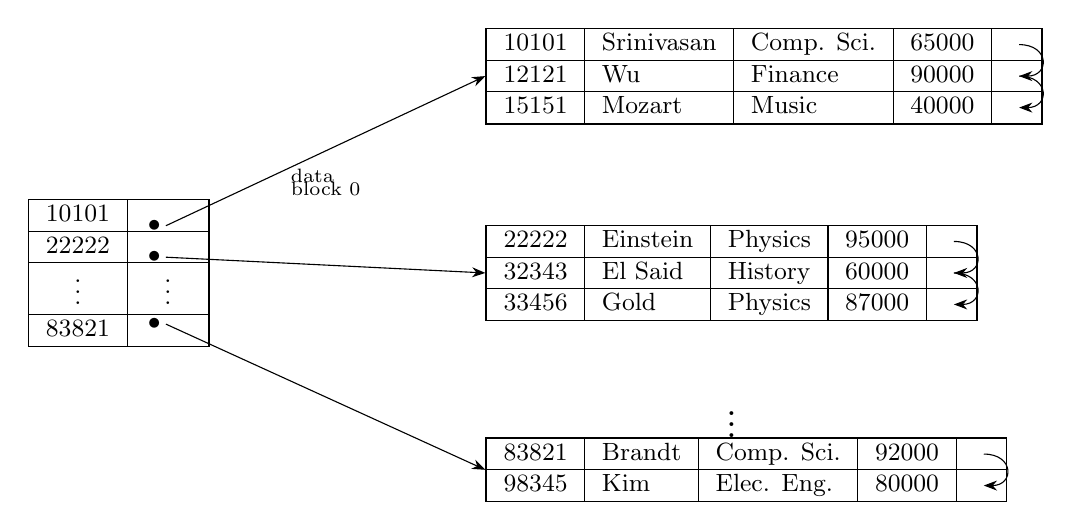
\begin{tikzpicture}[
        >=Stealth,
        table/.style={draw, inner sep=0pt},
        every node/.style={font=\small}
    ]

    % --- Index Table ---
    \node[table] (index) {
        \begin{tabular}{|c|c|}
            \hline
            10101 & \hspace{0.6cm} \\ \hline
            22222 & \\ \hline
            $\vdots$ & $\vdots$ \\ \hline
            83821 & \\ \hline
        \end{tabular}
    };
    
    % Add the bullet points (pointers) in the second column of the index table
    % Adjust coordinates slightly if your compiler renders tabular heights differently
    \node at (0.45, 0.6) {$\bullet$}; 
    \node at (0.45, 0.2) {$\bullet$}; 
    \node at (0.45, -0.65) {$\bullet$}; 

    % --- Data Block 1 ---
    \node[table, right=3.5cm of index, yshift=2.5cm] (block1) {
        \begin{tabular}{|l|l|l|l|c|}
            \hline
            10101 & Srinivasan & Comp. Sci. & 65000 & \hspace{0.2cm} \\ \hline
            12121 & Wu & Finance & 90000 & \\ \hline
            15151 & Mozart & Music & 40000 & \\ \hline
        \end{tabular}
    };

    % --- Data Block 2 ---
    \node[table, right=3.5cm of index, yshift=0cm] (block2) {
        \begin{tabular}{|l|l|l|l|c|}
            \hline
            22222 & Einstein & Physics & 95000 & \hspace{0.2cm} \\ \hline
            32343 & El Said & History & 60000 & \\ \hline
            33456 & Gold & Physics & 87000 & \\ \hline
        \end{tabular}
    };

    % Vertical Dots between Block 2 and 3
    \node[yshift=-1.2cm] at (block2.south) {\Large $\vdots$};

    % --- Data Block 3 ---
    \node[table, right=3.5cm of index, yshift=-2.5cm] (block3) {
        \begin{tabular}{|l|l|l|l|c|}
            \hline
            83821 & Brandt & Comp. Sci. & 92000 & \hspace{0.2cm} \\ \hline
            98345 & Kim & Elec. Eng. & 80000 & \\ \hline
        \end{tabular}
    };

    % --- Main Pointer Arrows (Index to Data Blocks) ---
    \draw[->] (0.6, 0.6) -- node[below, font=\scriptsize, align=left, yshift=-0.1cm] {data \\[-3pt] block 0} (block1.west);
    \draw[->] (0.6, 0.2) -- (block2.west);
    \draw[->] (0.6, -0.65) -- (block3.west);

    % --- Linked List Pointers (Curved Arrows inside Data Blocks) ---
    % Data Block 1 pointers
    \draw[->] ([yshift=0.4cm, xshift=-0.3cm]block1.east) to[out=0, in=0, looseness=2.5] ([yshift=0cm, xshift=-0.3cm]block1.east);
    \draw[->] ([yshift=0cm, xshift=-0.3cm]block1.east) to[out=0, in=0, looseness=2.5] ([yshift=-0.4cm, xshift=-0.3cm]block1.east);

    % Data Block 2 pointers
    \draw[->] ([yshift=0.4cm, xshift=-0.3cm]block2.east) to[out=0, in=0, looseness=2.5] ([yshift=0cm, xshift=-0.3cm]block2.east);
    \draw[->] ([yshift=0cm, xshift=-0.3cm]block2.east) to[out=0, in=0, looseness=2.5] ([yshift=-0.4cm, xshift=-0.3cm]block2.east);

    % Data Block 3 pointers
    \draw[->] ([yshift=0.2cm, xshift=-0.3cm]block3.east) to[out=0, in=0, looseness=2.5] ([yshift=-0.2cm, xshift=-0.3cm]block3.east);

    \end{tikzpicture}
\end{center}


\medskip
\begin{center}
\small
\begin{tabular}{llll}
\toprule
\textbf{ID} & \textbf{Name} & \textbf{Dept\_name} & \textbf{Salary}\\
\midrule
12122 & Rafique & History     & 40000\\
83820 & Abid    & Comp.\ Sci. & 90000\\
\bottomrule
\end{tabular}
\end{center}
\mk{10} \yr{CSE 215 | L-2/T-2 | 2020--21}

%% Q6 — 2020-21 primary vs secondary index comparison
\item Compare primary index with secondary index showing representative index structures.
\mk{10} \yr{CSE 215 | L-2/T-2 | 2020--21}

\end{enumerate}

%%──────────────────────────────────────────────────────────────────────
\subtopic{cD}{Secondary \& Bitmap Index}
\label{sub:s5-secondary}

\begin{enumerate}

%% Q1
\item The relation \texttt{account} is given in Figure 1. Construct bitmap indices on \texttt{type}, \texttt{branchname} and \texttt{location} attribute. Explain how you can find balance for $\text{branchname} = \text{`B2'}$ and $\text{location} = \text{`L1'}$ and $\text{type} = \text{`D'}$.
\mk{10} \yr{CSE 215 | L-3/T-1 | 2010--11}

%% Q2
\item Give an example where the Bitmap index is preferred over other indexing techniques.
\mk{5} \yr{CSE 303 | L-3/T-1 | 2012--13}

%% Q3 — 2014-15 bitmap on employee
\item Given the relation \texttt{employee(emp\_id, name, gender, status)}, create bitmap indices on \texttt{gender} and \texttt{status}.

\begin{center}
  \renewcommand{\arraystretch}{1.3} % Adds padding to match the image layout
    \begin{tabular}{|c|c|c|c|}
        \hline
        E001 & Abid   & Male & Full Time \\ \hline
        E002 & Arif   & Male & Full Time \\ \hline
        E003 & Sajid  & Male & Full Time \\ \hline
        E004 & Rafiq  & Male & Part Time \\ \hline
        E005 & Shahid & Male & Full Time \\ \hline
        E006 & Sajid  & Male & Full Time \\ \hline
        E007 & Karim  & Male & Part Time \\ \hline
        E008 & Zahid  & Male & Full Time \\ \hline
    \end{tabular}
    
    \vspace{0.4cm}
    \textbf{Figure 3:} File containing records of relation \textit{employee}(\textit{emp\_id}, \textit{name}, \textit{gender}, \textit{status})
\end{center}

\mk{5} \yr{CSE 303 | L-3/T-1 | 2014--15}

%% Q4 — 2015-16 bitmap short note
\item Write a short note on bitmap indexing.
\mk{5} \yr{CSE 303 | L-3/T-1 | 2015--16}

%% Q5 — 2016-17 unclustered sparse index
\item Is it possible to implement an unclustered-sparse indexing scheme? If so, give an example. Otherwise, briefly explain the reason.
\mk{6} \yr{CSE 303 | L-3/T-1 | 2016--17}

%% Q6 — 2017-18 bitmap preferred
\item Give an example where the Bit-map index is preferred over other indexing techniques.
\mk{5} \yr{CSE 215 | L-2/T-2 | 2017--18}

%% Q7 — 2018-19 secondary index query cost
\item The Employee Management System has schema \texttt{employee(e\_id, name, date\_of\_birth, salary, street, thana, district, NID)}. Total employees: 40,000; relation size: 4,000 blocks. Primary index: \texttt{e\_id}; secondary indices: \texttt{name}, \texttt{district}, \texttt{NID} with heights 3, 2, 4 respectively. Transfer time: 0.5 ms/block; average seek time: 8 ms. Tuples with \texttt{salary = 50000}: 100; \texttt{district = 'Comilla'}: 2000 (each tuple in a different block).

Find the query costs using indices for:
\[\texttt{SELECT * FROM employee WHERE salary = 50000 OR district = 'Comilla'}\]
 \mk{8} \yr{CSE 215 | L-2/T-2 | 2018--19}

%% Q8 — 2019-20 ordered secondary index with bucket overflow + insertion
\item A relation schema $R(A, B, C)$ and a relation $r(R)$ is given below. The relation is physically sorted on the primary key $A$. Construct an ordered secondary index of $r$ on attribute $B$ considering the buckets containing maximum 3 pointers. Explain the cases if you need to insert the tuple $t = \langle a_8, b_2, c_2 \rangle$.

\medskip
\begin{center}
\small
\begin{tabular}{lll}
\toprule
\textbf{A} & \textbf{B} & \textbf{C}\\
\midrule
$a_1$ & $b_1$ & $c_1$\\
$a_2$ & $b_2$ & $c_1$\\
$a_3$ & $b_3$ & $c_1$\\
$a_4$ & $b_1$ & $c_1$\\
$a_5$ & $b_2$ & $c_1$\\
$a_7$ & $b_2$ & $c_1$\\
$a_8$ & $b_3$ & $c_1$\\
\bottomrule
\end{tabular}
\end{center}
\mk{15} \yr{CSE 215 | L-2/T-2 | 2019--20}

%% Q9 — 2020-21 conjunctive selection with secondary B+ tree indices (worst case cost)
\item The \texttt{student} relation has schema \texttt{Student(Id, name, f\_name, m\_name, cgpa, year\_admit, division, district, thana, street, house\_number, city, NID, DOB, total\_credit)}. B$^+$ tree secondary indices exist on \texttt{name}, \texttt{city}, and \texttt{year\_admit} with heights 4, 2 and 1 respectively. The number of tuples for \texttt{name = 'Abid'}, \texttt{City = 'Feni'}, and \texttt{year\_admit = 2015} are 50, 20 and 1000 respectively. Seek cost: 10 ms, block transfer cost: 0.1 ms. Number of blocks of student relation: 2000.

\begin{enumerate}
  \item Find the worst-case costs of processing the following conjunctive selection query using the single index method:
  \[\texttt{SELECT * FROM student WHERE name = 'Abid' AND City = 'Feni' AND year\_admit = 2015}\]
  \item Explain clearly how this query will be executed in this method.
\end{enumerate}
 \mk{10} \yr{CSE 215 | L-2/T-2 | 2020--21}

%% Q10 — 2021-22 bitmap index vs linear file scan
\item ``Without bitmap index scan strategy, secondary index scan can sometimes perform worse than linear file scan.'' --- Justify or criticize this statement with proper explanation.
\mk{15} \yr{CSE 215 | L-2/T-2 | 2021--22}

\end{enumerate}

%%──────────────────────────────────────────────────────────────────────
\subtopic{cD}{B\textsuperscript{+} Tree Index}
\label{sub:s5-btree}

\begin{enumerate}

%% Q1
\item Construct a B$^+$ tree for the set of key values $\{2, 4, 6, 8, 12, 18, 20, 24, 30, 32\}$ with $n = 4$. Assume that the tree is initially empty and values are added in the given order.
\mk{10} \yr{CSE 215 | L-3/T-1 | 2010--11}

%% Q2
\item Write down the key properties of a B$^+$-tree.
\mk{8} \yr{CSE 303 | L-3/T-1 | 2011--12}

%% Q3
\item Draw a B$^+$-tree for the following keys: 2, 3, 5, 7, 14, 16, 20, 34, 38, and 40. Assume a 2-order B$^+$-tree where a node must have 2 to 4 keys. Re-construct the tree after deleting 3, 5, and 7 from the original tree.
\mk{15} \yr{CSE 303 | L-3/T-1 | 2011--12}

%% Q4
\item Suppose in a B$^+$-tree, pointers are 4 bytes long and keys are 12 bytes long. How many keys and pointers will a block of 16,384 bytes have? For a one million record table, what would be the expected length of the index?
\mk{12} \yr{CSE 303 | L-3/T-1 | 2011--12}

\variant{CSE 215 | L-3/T-1 | 2012--13 (same pointer/key sizes, 16384 byte block)}

%% Q5
\item Draw the B-tree to index the following elements: 2, 3, 5, 13, 17, 19, 23, 29, 31, 37, 41, 43, and 47. Delete elements 31 and 43 and redraw the tree.
\mk{17} \yr{CSE 303 | L-3/T-1 | 2012--13}

%% Q6 — 2015-16 B+ tree given final structure
\item Show the final B$^+$ tree index structure for the search key values 2, 4, 6, 8, 10, 12, 14, 16, 18, 20, 22, 24 with 4 leaf nodes and $n = 4$. (You do not need to create this index step by step.) Then show the index structure after insertion of 15.
\mk{20} \yr{CSE 303 | L-3/T-1 | 2015--16}

%% Q7 — 2014-15 B+ tree principles
\item Discuss the basic principles of B$^+$ tree index structure.
\mk{10} \yr{CSE 303 | L-3/T-1 | 2014--15}

%% Q8 — 2013-14 B+ tree comparison
\item Compare Hash-based index, B$^+$-tree index, and Bitmap index.
\mk{6} \yr{CSE 303 | L-3/T-1 | 2013--14}

%% Q9 — 2016-17 B+ tree insert and delete operations
\item Consider a B$^+$ tree with leaf nodes: $\{2,3,5\}$, $\{14,16\}$, $\{19,20,22\}$, $\{24,27,29\}$, $\{33,34,38,39\}$. Show (without explanation) what happens after each of the following successive operations:
\begin{enumerate}
  \item Insert 7
  \item Insert 8
  \item Delete 19
  \item Delete 20
\end{enumerate}

\begin{center}
  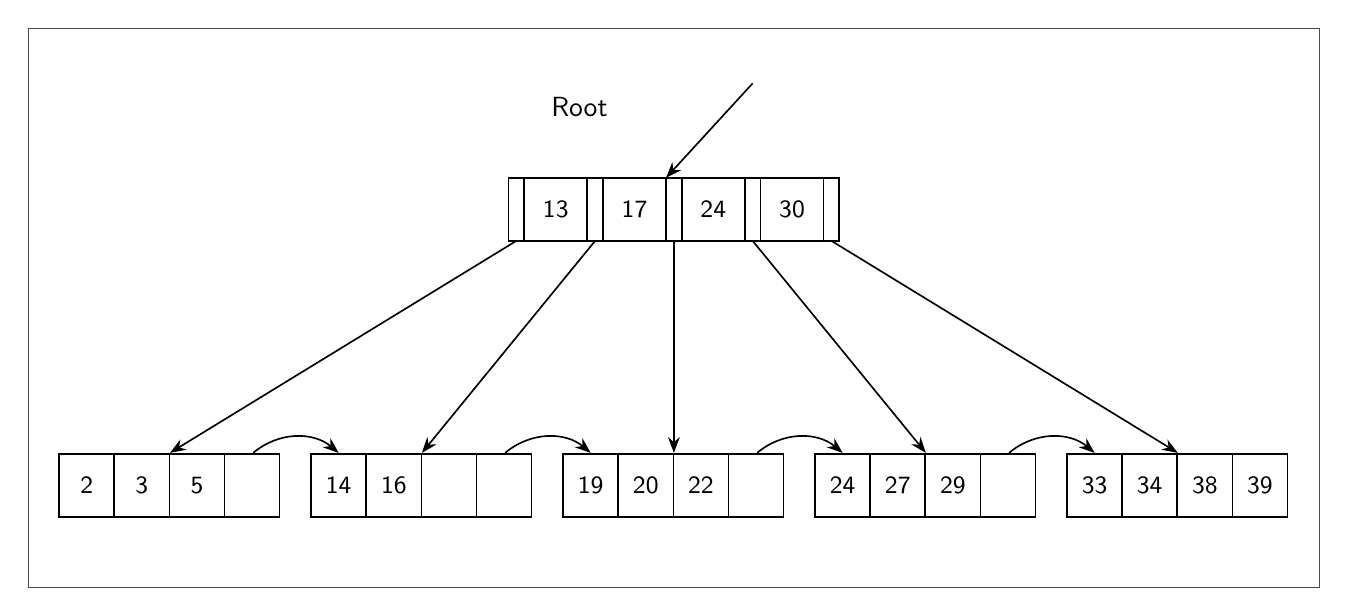
\begin{tikzpicture}[
        >=Stealth,
        arrow_style/.style={->, line width=0.6pt}
    ]

    % =========================================================================
    % 1. LEAF NODES (Bottom Level)
    % =========================================================================
    % Spaced consistently horizontally by 3.2cm centers
    \leafnode{L1}{-6.4, -3.5}{2}{3}{5}{}
    \leafnode{L2}{-3.2, -3.5}{14}{16}{}{}
    \leafnode{L3}{0, -3.5}{19}{20}{22}{}
    \leafnode{L4}{3.2, -3.5}{24}{27}{29}{}
    \leafnode{L5}{6.4, -3.5}{33}{34}{38}{39}

    % =========================================================================
    % 2. ROOT NODE
    % =========================================================================
    \begin{scope}[shift={(0,0)}]
        % Outer boundary for root node
        \draw[line width=0.6pt] (-2.1, -0.4) rectangle (2.1, 0.4);
        
        % Vertical dividers to create thin pointer slots and wide key slots
        \draw[line width=0.6pt] (-1.9, -0.4) -- (-1.9, 0.4); % P1 end
        \draw[line width=0.6pt] (-1.1, -0.4) -- (-1.1, 0.4); % K1 end
        \draw[line width=0.6pt] (-0.9, -0.4) -- (-0.9, 0.4); % P2 end
        \draw[line width=0.6pt] (-0.1, -0.4) -- (-0.1, 0.4); % K2 end
        \draw[line width=0.6pt] ( 0.1, -0.4) -- ( 0.1, 0.4); % P3 end
        \draw[line width=0.6pt] ( 0.9, -0.4) -- ( 0.9, 0.4); % K3 end
        \draw[line width=0.6pt] ( 1.1, -0.4) -- ( 1.1, 0.4); % P4 end
        \draw[line width=0.6pt] ( 1.9, -0.4) -- ( 1.9, 0.4); % K4 end
        
        % Key values in wide slots
        \node[font=\sffamily\small] at (-1.5, 0) {13};
        \node[font=\sffamily\small] at (-0.5, 0) {17};
        \node[font=\sffamily\small] at (0.5, 0) {24};
        \node[font=\sffamily\small] at (1.5, 0) {30};
        
        % Establish precise pointer origin coordinates (bottom center of thin slots)
        \coordinate (P1) at (-2.0, -0.4);
        \coordinate (P2) at (-1.0, -0.4);
        \coordinate (P3) at (0.0, -0.4);
        \coordinate (P4) at (1.0, -0.4);
        \coordinate (P5) at (2.0, -0.4);
    \end{scope}

    % =========================================================================
    % 3. TREE POINTERS (Root to Leaves)
    % =========================================================================
    \draw[arrow_style] (P1) -- (L1.north);
    \draw[arrow_style] (P2) -- (L2.north);
    \draw[arrow_style] (P3) -- (L3.north);
    \draw[arrow_style] (P4) -- (L4.north);
    \draw[arrow_style] (P5) -- (L5.north);

    % =========================================================================
    % 4. HORIZONTAL LEAF LINKS (Curved Arrows)
    % =========================================================================
    % Using out and in angles to create jumping arcs across the nodes
    \draw[arrow_style] ($(L1.north east)+(-0.35, 0)$) to[out=40, in=140] ($(L2.north west)+(0.35, 0)$);
    \draw[arrow_style] ($(L2.north east)+(-0.35, 0)$) to[out=40, in=140] ($(L3.north west)+(0.35, 0)$);
    \draw[arrow_style] ($(L3.north east)+(-0.35, 0)$) to[out=40, in=140] ($(L4.north west)+(0.35, 0)$);
    \draw[arrow_style] ($(L4.north east)+(-0.35, 0)$) to[out=40, in=140] ($(L5.north west)+(0.35, 0)$);

    % =========================================================================
    % 5. ROOT ANNOTATION & OUTER BOUNDARY
    % =========================================================================
    \node[font=\sffamily] at (-1.2, 1.3) {Root};
    \draw[arrow_style] (1.0, 1.6) -- (-0.1, 0.4);

    % Mimics the diagram's outer box frame
    \draw[line width=0.4pt, draw=black!70] (-8.2, -4.8) rectangle (8.2, 2.3);
    
    % Bottom text caption placed inside the frame 

    \end{tikzpicture}
\end{center}

\mk{8} \yr{CSE 303 | L-3/T-1 | 2016--17}

%% Q10 — 2016-17 key properties of B+ tree
\item Write down the key properties of a B$^+$ tree.
\mk{8} \yr{CSE 303 | L-3/T-1 | 2016--17}

\variant{2017--18: same question \mk{8}}

%% Q11 — 2017-18 B+ tree incremental modifications
\item Consider a given B$^+$ tree (Figure for Q4(c)). Modify it incrementally according to the following instructions. For each instruction, draw the final modified state:
\begin{enumerate}
  \item Insert keys 8, 9
  \item Insert keys 24, 27
  \item Remove keys 8, 9
  \item Remove keys 24, 27
\end{enumerate}

\begin{center}
  
    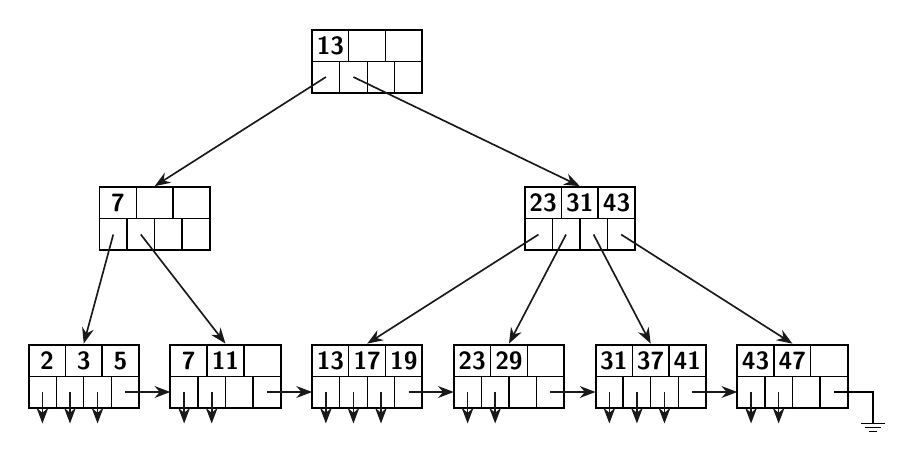
\begin{tikzpicture}[
        >=Stealth,
        arrow_style/.style={->, line width=0.6pt, draw=black!90}
    ]

    % =========================================================================
    % 1. NODE PLACEMENTS (Calculated mathematically for balanced spacing)
    % =========================================================================
    
    % Leaf Level Nodes (y = 0)
    \btnode{Leaf1}{(-4.5, 0)}{2}{3}{5}
    \btnode{Leaf2}{(-2.7, 0)}{7}{11}{}
    \btnode{Leaf3}{(-0.9, 0)}{13}{17}{19}
    \btnode{Leaf4}{(0.9, 0)}{23}{29}{}
    \btnode{Leaf5}{(2.7, 0)}{31}{37}{41}
    \btnode{Leaf6}{(4.5, 0)}{43}{47}{}

    % Level 1 Nodes (y = 2.0)
    \btnode{L1Left}{(-3.6, 2.0)}{7}{}{}
    \btnode{L1Right}{(1.8, 2.0)}{23}{31}{43}

    % Root Node (y = 4.0)
    \btnode{Root}{(-0.9, 4.0)}{13}{}{}


    % =========================================================================
    % 2. CONNECTING POINTERS (Tree Hierarchy Links)
    % =========================================================================
    
    % Root Pointers
    \draw[arrow_style] (Root-p0) -- (L1Left-top);
    \draw[arrow_style] (Root-p1) -- (L1Right-top);

    % Level 1 Left Pointers
    \draw[arrow_style] (L1Left-p0) -- (Leaf1-top);
    \draw[arrow_style] (L1Left-p1) -- (Leaf2-top);

    % Level 1 Right Pointers
    \draw[arrow_style] (L1Right-p0) -- (Leaf3-top);
    \draw[arrow_style] (L1Right-p1) -- (Leaf4-top);
    \draw[arrow_style] (L1Right-p2) -- (Leaf5-top);
    \draw[arrow_style] (L1Right-p3) -- (Leaf6-top);


    % =========================================================================
    % 3. LEAF LEVEL HORIZONTAL POINTERS
    % =========================================================================
    \draw[arrow_style] (Leaf1-p3) -- (Leaf2-leftbtm);
    \draw[arrow_style] (Leaf2-p3) -- (Leaf3-leftbtm);
    \draw[arrow_style] (Leaf3-p3) -- (Leaf4-leftbtm);
    \draw[arrow_style] (Leaf4-p3) -- (Leaf5-leftbtm);
    \draw[arrow_style] (Leaf5-p3) -- (Leaf6-leftbtm);

    % Leaf 6 Ground Terminal Connection
    \draw[line width=0.6pt] (Leaf6-p3) -- ++(0.5, 0) -- ++(0, -0.4) coordinate (gnd);
    \draw[line width=0.6pt] ($(gnd)+(-0.15, 0)$) -- ($(gnd)+(0.15, 0)$);
    \draw[line width=0.6pt] ($(gnd)+(-0.10, -0.05)$) -- ($(gnd)+(0.10, -0.05)$);
    \draw[line width=0.6pt] ($(gnd)+(-0.05, -0.10)$) -- ($(gnd)+(0.05, -0.10)$);


    % =========================================================================
    % 4. DOWNWARD DATA POINTERS (Under active key elements)
    % =========================================================================
    
    % Leaf 1 Pointers
    \draw[arrow_style] (Leaf1-p0) -- ++(0, -0.4);
    \draw[arrow_style] (Leaf1-p1) -- ++(0, -0.4);
    \draw[arrow_style] (Leaf1-p2) -- ++(0, -0.4);

    % Leaf 2 Pointers
    \draw[arrow_style] (Leaf2-p0) -- ++(0, -0.4);
    \draw[arrow_style] (Leaf2-p1) -- ++(0, -0.4);

    % Leaf 3 Pointers
    \draw[arrow_style] (Leaf3-p0) -- ++(0, -0.4);
    \draw[arrow_style] (Leaf3-p1) -- ++(0, -0.4);
    \draw[arrow_style] (Leaf3-p2) -- ++(0, -0.4);

    % Leaf 4 Pointers
    \draw[arrow_style] (Leaf4-p0) -- ++(0, -0.4);
    \draw[arrow_style] (Leaf4-p1) -- ++(0, -0.4);

    % Leaf 5 Pointers
    \draw[arrow_style] (Leaf5-p0) -- ++(0, -0.4);
    \draw[arrow_style] (Leaf5-p1) -- ++(0, -0.4);
    \draw[arrow_style] (Leaf5-p2) -- ++(0, -0.4);

    % Leaf 6 Pointers
    \draw[arrow_style] (Leaf6-p0) -- ++(0, -0.4);
    \draw[arrow_style] (Leaf6-p1) -- ++(0, -0.4);

    \end{tikzpicture}
\end{center}

\mk{16} \yr{CSE 215 | L-2/T-2 | 2017--18}

%% Q12 — 2019-20 B+ tree primary index for relation r, n=3, insert a6
\item Construct a B$^+$ tree primary index for the relation $r$ of question 2(a) (relation $R(A,B,C)$ sorted on primary key $A$, with keys $a_1, a_2, a_3, a_4, a_5, a_7, a_8$) with $n = 3$ by insertion of search keys incrementally in sorted order and splitting of nodes. After construction of the tree, insert $a_6$ and show the tree structure.
\mk{20} \yr{CSE 215 | L-2/T-2 | 2019--20}

%% Q13 — 2020-21 B+ tree n=4, insert 90 down to 20, then delete 20,30,40,50
\item
\begin{enumerate}
  \item Construct a B$^+$ tree index structure with $n = 4$, incrementally inserting the search keys 90, 80, 70, 60, 50, 40, 30, 20.
  \item Show the structures after deletion of 20, 30, 40 and 50.
\end{enumerate}
\mk{20} \yr{CSE 215 | L-2/T-2 | 2020--21}

%% Q14 — 2022-23 degree-3 B+ tree: insert 315, 409, 513; delete 456, 513, 982, 895
\item The following is a degree-3 B$^+$ tree created after some insert/delete operations:
\begin{center}

  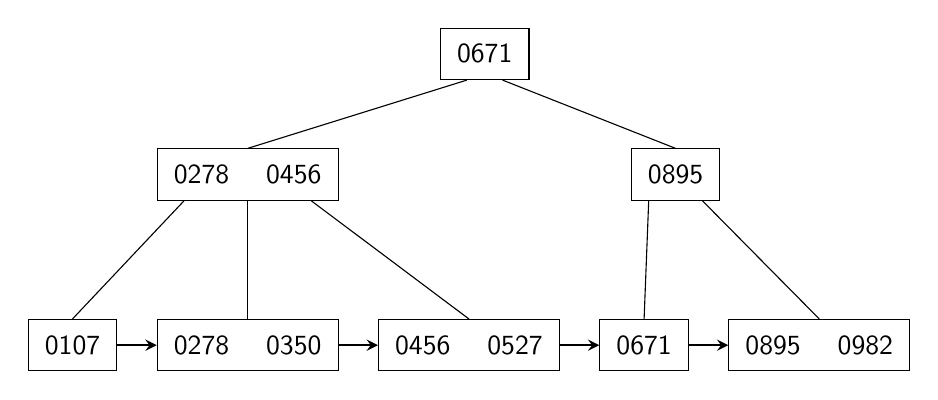
\begin{tikzpicture}[
  bnode/.style={draw, rectangle, minimum height=0.6cm, inner sep=6pt, font=\sffamily},
  >=stealth
]
  % 1. Leaf nodes (Bottom Level)
  \node[bnode] (l1) {0107};
  \node[bnode, right=0.5cm of l1] (l2) {0278 \quad 0350};
  \node[bnode, right=0.5cm of l2] (l3) {0456 \quad 0527};
  \node[bnode, right=0.5cm of l3] (l4) {0671};
  \node[bnode, right=0.5cm of l4] (l5) {0895 \quad 0982};

  % Leaf node horizontal arrows (linked list behavior)
  \draw[->, thick] (l1.east) -- (l2.west);
  \draw[->, thick] (l2.east) -- (l3.west);
  \draw[->, thick] (l3.east) -- (l4.west);
  \draw[->, thick] (l4.east) -- (l5.west);

  % 2. Intermediate Level nodes
  \node[bnode, above=1.5cm of l2] (n1) {0278 \quad 0456};
  \node[bnode, above=1.5cm of l4, xshift=0.4cm] (n2) {0895}; 

  % 3. Root node
  \path (n1) -- (n2) coordinate[midway] (mid);
  \node[bnode, above=1.2cm of mid] (root) {0671};

  % 4. Draw Edges from Root to Level 1
  % Calculating exact points on the bottom of the box for standard B-Tree look
  \draw ($ (root.south west) !0.3! (root.south east) $) -- (n1.north);
  \draw ($ (root.south west) !0.7! (root.south east) $) -- (n2.north);

  % 5. Draw Edges from n1 (0278 | 0456) to leaves
  \draw ($ (n1.south west) !0.15! (n1.south east) $) -- (l1.north);
  \draw ($ (n1.south west) !0.5! (n1.south east) $) -- (l2.north);
  \draw ($ (n1.south west) !0.85! (n1.south east) $) -- (l3.north);

  % 6. Draw Edges from n2 (0895) to leaves
  \draw ($ (n2.south west) !0.2! (n2.south east) $) -- (l4.north);
  \draw ($ (n2.south west) !0.8! (n2.south east) $) -- (l5.north);

\end{tikzpicture}

\end{center}
Draw the state of this B$^+$ tree after each of the following operations:
\begin{enumerate}
  \item Insert 315
  \item Insert 409 and 513
  \item Delete 456
  \item Delete 513
  \item Delete 982 and 895
\end{enumerate}
\mk{20} \yr{CSE 215 | L-2/T-1 | 2022--23}

%% Q15 — 2022-23 height of degree-5 B+ tree for 1 to 100
\item For a degree-5 B$^+$ tree, what will be the height of the B$^+$ tree when the numbers from 1 to 100 are inserted sequentially? \textit{Hint:} A tree with $l$ leaves and internal nodes of degree $d$ has height approximately $\log_d l$.
\mk{5} \yr{CSE 215 | L-2/T-1 | 2022--23}

%% Q16 — 2024-25 B+ tree n=4 (order 4): 10 million records, node size 4KB
\item Given a B$^+$ tree index with 10 million records, node size = 4 kilobytes, search-key size = 8 bytes, disk-pointer size = 4 bytes. Answer the following:
\begin{enumerate}
  \item Given a search-key, how many index blocks need to be read from disk in the best case to find the pointer to the data record?
  \item Given a range query assuming 1000 records will be retrieved, how many index blocks need to be read in the best case?
  \item Given a search-key, how many index blocks need to be read in the best and worst cases if we use a hash index instead? Assume the hash index requires at most three overflow blocks.
\end{enumerate}
\mk{15} \yr{CSE 215 | L-2/T-1 | 2024--25}

%% Q17 — 2024-25 B+ tree n=4: insert 2,3,5,7,11,17,19,23,29,31; delete 23,19
\item Assume a B$^+$ tree index is initially empty and the number of pointers that fit in one node is 4.
\begin{enumerate}
  \item Construct the tree by inserting the following key values in the given order: 2, 3, 5, 7, 11, 17, 19, 23, 29, 31.
  \item Show the final form of the tree after: Delete 23, Delete 19.
\end{enumerate}
\mk{13} \yr{CSE 215 | L-2/T-1 | 2024--25}

\end{enumerate}

%%──────────────────────────────────────────────────────────────────────
\subtopic{cD}{Hash Index}
\label{sub:s5-hash}

\begin{enumerate}

%% Q1
\item Describe static hash file organization with an example. How can bucket overflows be handled?
\mk{10} \yr{CSE 215 | L-3/T-1 | 2010--11}

%% Q2
\item Discuss Linear Hashing and Extensible Hashing with examples. How do they differ from each other?
\mk{13} \yr{CSE 303 | L-3/T-1 | 2012--13}

%% Q3 — 2015-16 dynamic hash index on balance
\item Construct the dynamic hash index structure on the \texttt{balance} attribute for the customer relation (records C0001--C0010, balances 1000--10000). The binary representation of the most significant digit of balance is the hash code. Insert records in descending order of balance.


\medskip
\begin{center}
\small
\begin{tabular}{llllll}
\toprule
\textbf{Record} & \textbf{CustID} & \textbf{Name} & \textbf{Street} & \textbf{City} & \textbf{Balance}\\
\midrule
0 & C0001 & N1 & North & Dhaka & 1000\\
1 & C0002 & N2 & North & Dhaka & 2000\\
2 & C0003 & N3 & North & Dhaka & 3000\\
3 & C0004 & N4 & North & Dhaka & 4000\\
4 & C0005 & N5 & North & Dhaka & 5000\\
5 & C0006 & N6 & South & Dhaka & 6000\\
6 & C0007 & N7 & South & Dhaka & 7000\\
7 & C0008 & N8 & South & Dhaka & 8000\\
8 & C0009 & N9 & South & Dhaka & 9000\\
9 & C0010 & N10 & South & Dhaka & 10000\\
\bottomrule
\end{tabular}
\end{center}

\mk{20} \yr{CSE 303 | L-3/T-1 | 2015--16}

%% Q4 — 2014-15 dynamic hash on employee name
\item Given the \texttt{employee(emp\_id, name, gender, status)} relation with hash values on \texttt{name}, create step by step a dynamic hash index structure for \texttt{name}. Assume a bucket can contain only one record and an overflow bucket can be used.


\begin{center}
  \renewcommand{\arraystretch}{1.3} % Adds padding to match the image layout
    \begin{tabular}{|c|c|c|c|}
        \hline
        E001 & Abid   & Male & Full Time \\ \hline
        E002 & Arif   & Male & Full Time \\ \hline
        E003 & Sajid  & Male & Full Time \\ \hline
        E004 & Rafiq  & Male & Part Time \\ \hline
        E005 & Shahid & Male & Full Time \\ \hline
        E006 & Sajid  & Male & Full Time \\ \hline
        E007 & Karim  & Male & Part Time \\ \hline
        E008 & Zahid  & Male & Full Time \\ \hline
    \end{tabular}
    
    \vspace{0.4cm}
    \textbf{Figure 3:} File containing records of relation \textit{employee}(\textit{emp\_id}, \textit{name}, \textit{gender}, \textit{status})
\end{center}
\vspace{0.5cm}
\begin{center}
  \renewcommand{\arraystretch}{1.3} % Adds padding to match the image layout
    \begin{tabular}{|c|c|}
        \hline
        \textbf{Name} & \textbf{16 bit hash code $h$(Name)} \\ \hline
        Abid   & 0001111100001111 \\ \hline
        Arif   & 0010111100001111 \\ \hline
        Sajid  & 0011111100001111 \\ \hline
        Rafiq  & 0100111100001111 \\ \hline
        Shahid & 0101111100001111 \\ \hline
        Karim  & 1001111100001111 \\ \hline
        Zahid  & 0111111100001111 \\ \hline
    \end{tabular}
    
    \vspace{0.4cm}
    \textbf{Figure 4:} The list of names of figure 3 and corresponding 16 bit hash codes.
\end{center}

\mk{15} \yr{CSE 303 | L-3/T-1 | 2014--15}

%% Q5 — 2013-14 linear hashing
\item Show the state of the linear hashing after inserting items: 0000, 0011, 0010, 0101, 1010, 1011, 1110, and 1111. Then show the state after inserting 1101 and 0111 into the hash table.
\mk{14} \yr{CSE 303 | L-3/T-1 | 2013--14}

%% Q6 — 2016-17 good hash function
\item What is the key property of a good hash function? How can you choose such a function?
\mk{6} \yr{CSE 303 | L-3/T-1 | 2016--17}

%% Q7 — 2016-17 linear hash table step-by-step
\item The following figure shows a linear hash table with 3 records. We assume hash function $h$ produces 4 bits and we represent records by the value produced by $h$ when applied to the search key of the record. Here, $i$ is the number of lower order bits of the hash function currently used and $n$ is the current number of buckets. Each bucket can hold maximum of 2 records. We shall adopt the policy of choosing $n$, so that there are no more than $1.7 n$ records in the file.

\vspace{0.6cm}

\begin{center}
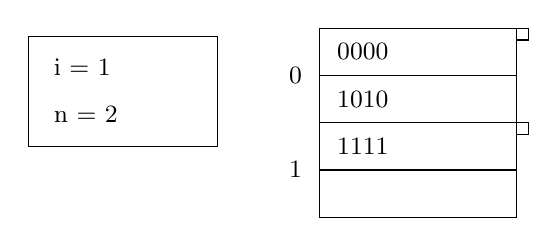
\begin{tikzpicture}[font=\small]
    
    % 1. Left parameter box
    % Centered vertically relative to the buckets
    \node[draw, rectangle, minimum width=2.4cm, minimum height=1.4cm] (box) at (0, 0) {};
    \node[anchor=west] at (-1.0, 0.3) {i = 1};
    \node[anchor=west] at (-1.0, -0.3) {n = 2};

    % 2. Bucket structural coordinates
    % Offset to the right to leave space between box and buckets
    \def\bx{2.5}
    \def\topY{0.8}

    % 3. Bucket 0
    % Main bucket outline
    \draw (\bx, \topY) rectangle (\bx+2.5, \topY-1.2);
    % Center divider for the two slots
    \draw (\bx, \topY-0.6) -- (\bx+2.5, \topY-0.6);
    % Slot records
    \node[anchor=west] at (\bx+0.1, \topY-0.3) {0000};
    \node[anchor=west] at (\bx+0.1, \topY-0.9) {1010};
    % Bucket Label
    \node[anchor=east] at (\bx-0.1, \topY-0.6) {0};
    % Small overflow/tab indicator top right
    \draw (\bx+2.5, \topY) rectangle (\bx+2.65, \topY-0.15);

    % 4. Bucket 1
    \def\bby{-0.4} % Top of bucket 1 is exactly at the bottom of bucket 0
    % Main bucket outline
    \draw (\bx, \bby) rectangle (\bx+2.5, \bby-1.2);
    % Center divider for the two slots
    \draw (\bx, \bby-0.6) -- (\bx+2.5, \bby-0.6);
    % Slot records
    \node[anchor=west] at (\bx+0.1, \bby-0.3) {1111};
    % Bucket Label
    \node[anchor=east] at (\bx-0.1, \bby-0.6) {1};
    % Small overflow/tab indicator top right
    \draw (\bx+2.5, \bby) rectangle (\bx+2.65, \bby-0.15);

\end{tikzpicture}
\end{center}
Now, show (step by step) what happens after successive insertion of 0101, 0001 and
0111. Show the necessary calculation whenever a new bucket is required. Overflow
blocks can be used if necessary.
\mk{15} \yr{CSE 303 | L-3/T-1 | 2016--17}

%% Q8 — 2017-18 extensible hashing with product table
\item Insert all the following data incrementally using the Product Id in an initially empty extensible hashing system using hash function $h(x) = x \bmod 1024$. Show the state of the system after each insertion:

\medskip
\begin{center}
\begin{tabular}{lll}
\toprule
\textbf{Product Id} & \textbf{Quantity} & \textbf{Price per Qty}\\
\midrule
03 & 10 & 5\\
05 & 5 & 90\\
09 & 10 & 1200\\
11 & 12 & 50\\
13 & 11 & 89\\
18 & 2 & 65\\
\bottomrule
\end{tabular}
\end{center}
\mk{9} \\

Insert all the data from the product table above, incrementally using the Product Id in an initially empty linear hashing system. Show the state of the system after each insertion.
\mk{12} \yr{CSE 215 | L-2/T-2 | 2017--18}

%% Q10 — 2021-22 extendable hashing h(x)=x mod 7, bucket size 3
\item Suppose that extendable hashing is being used on a database file that contains records with the following search key values: 2, 3, 5, 7, 11, 17, 19, and 23. Construct the extendable hash structure for this file if the hash function is $h(x) = x \bmod 7$ and each bucket can hold at most three records.
\mk{15} \yr{CSE 215 | L-2/T-2 | 2021--22}

\end{enumerate}

%% ── S6: Query Processing ──────────────────────────────────────────────
\section{S6 --- Query Processing}
\label{sec:S6}
\markboth{S6 --- Query Processing}{}

%%──────────────────────────────────────────────────────────────────────
\subtopic{cD}{Query Processing}
\label{sub:s6-qp}

\begin{enumerate}

%% Q1
\item Discuss the subsystems that are related to query processing in a Database Management System (DBMS).
\mk{10} \yr{CSE 303 | L-3/T-1 | 2012--13}

%% Q2
\item Write the steps of performing a one-pass algorithm for finding the maximum value of an attribute for relation $R$. If the buffer size is $M$, what is the relationship between $R$ and $M$? Derive the relationship between $M$ and $R$ for a two-pass aggregate operation.
\mk{20} \yr{CSE 303 | L-3/T-1 | 2012--13}

%% Q3
\item Derive the total number of disk I/Os for nested loop join of two relations $R$ and $S$, where the number of records in $R$ is smaller than the number of records in $S$.
\mk{5} \yr{CSE 303 | L-3/T-1 | 2012--13}

%% Q4 — 2014-15 external sort-merge
\item Explain external sort-merge with an example. Show that the total number of block transfers for external sorting of a relation $r$ is:
\[b_r\!\left(2\left\lceil\log_{M-1}(C\dfrac{b_r}{M})\right\rceil + 1\right)\]
where $b_r$ is the number of blocks of relation $r$ and $M$ is the size of the main memory buffer.
\mk{15} \yr{CSE 303 | L-3/T-1 | 2014--15}

%% Q5 — 2014-15 nested/block nested loop join cost
\item Let relation $r_1(A, B, C)$ and $r_2(C, D, E)$ have the following properties: $r_1$ has 20,000 tuples, $r_2$ has 45,000 tuples, 25 tuples of $r_1$ fit on one block, and 30 tuples of $r_2$ fit on one block. Estimate the number of block transfers and seeks required using:
\begin{enumerate}
  \item Nested loop join.
  \item Block nested loop join.
\end{enumerate}
\mk{10} \yr{CSE 303 | L-3/T-1 | 2014--15}

%% Q6 — 2014-15 B+ tree query cost
\item Let $t_r$ and $t_s$ be the time to transfer a block of data and the time to seek a block in a disk subsystem, respectively. Estimate the query processing cost for:
\begin{enumerate}
  \item A primary B$^+$ tree index and equality on key.
  \item A primary B$^+$ tree index and comparison on key.
\end{enumerate}
\mk{10} \yr{CSE 303 | L-3/T-1 | 2014--15}

%% Q7 — 2013-14 two-phase multiway merge sort
\item Write down the steps of two-phase multiway merge sort. Consider a system where the block size is $B$ bytes, memory size is $M$ bytes, and record size is $R$ bytes. What is the maximum number of records that can be sorted using two-phase merge sort? If the number of records exceeds this maximum, how can you sort them?
\mk{15} \yr{CSE 303 | L-3/T-1 | 2013--14}

%% Q8 — 2013-14 duplicate elimination
\item Show the steps of duplicate elimination using a two-pass algorithm. Derive the relationship between number of records and memory size in this algorithm.
\mk{15} \yr{CSE 303 | L-3/T-1 | 2013--14}

%% Q9 — 2016-17 sort-based union algorithm
\item Write down the pseudocode for a sort-based union algorithm that computes $R \cup S$. Also mention its runtime and constraints in terms of $B(R)$, $B(S)$ and $M$, where $B(R)$ and $B(S)$ are the number of blocks in $R$ and $S$, and $M$ is the number of blocks of each sublist to be sorted.
\mk{12} \yr{CSE 303 | L-3/T-1 | 2016--17}

%% Q10 — 2017-18 one-pass algorithm for set difference
\item Write the steps of a one-pass algorithm for finding $S - R$, where the number of records in relation $R$ is smaller than the number of records in relation $S$.
\mk{6} \yr{CSE 215 | L-2/T-2 | 2017--18}

%% Q11 — 2018-19 external sort-merge diagram
\item An unsorted relation \texttt{r\_unsorted} has 36 blocks (B1--B36) and the memory size for external sort-merge is 4 blocks. Show the diagram to sort the relation using the external sort-merge algorithm and store it as \texttt{r\_sorted}. Using the diagram, explain the total number of block transfers needed to sort the relation and store it.
  \mk{15} \yr{CSE 215 | L-2/T-2 | 2018--19}

%% Q12 — 2018-19 OR query cost with secondary indices
\item Explain the algorithm used to process the following SQL query given secondary indices on \texttt{salary} and \texttt{district}:
\[\texttt{SELECT * FROM employee WHERE salary = 50000 OR district = 'Comilla'}\]
\mk{7} \yr{CSE 215 | L-2/T-2 | 2018--19}

%% Q13 — 2019-20 external sort-merge: runs, passes, transfers, seeks
\item Memory size is $M$ blocks and the number of blocks of a relation $r$ is $b_r$. Find the number of runs $N$, number of merge passes, number of block transfers, and number of seeks to sort the relation $r$ using the external sort-merge algorithm for the following cases:
\begin{enumerate}
  \item Case 1: $N < M$
  \item Case 2: $N = M$
  \item Case 3: $N > M$
\end{enumerate}
\mk{15} \yr{CSE 215 | L-2/T-2 | 2019--20}

%% Q14 — 2021-22 aggregation and set operations pipelining
\item Describe how aggregation and set operations of an SQL query are processed and whether pipelining can improve their performance.
\mk{10} \yr{CSE 215 | L-2/T-2 | 2021--22}

%% Q15 — 2023-24 two-pass grouping/aggregation using sorting + sort-based union cost
\item Describe the two-pass algorithm for grouping and aggregation using sorting. Suppose the number of blocks in relation $R$ is 50,000 and in relation $S$ is 20,000. Compute the memory and I/O cost for the sort-based union operation $R \cup S$.
\mk{14} \yr{CSE 215 | L-2/T-1 | 2023--24}

%% Q16 — 2024-25 sort-merge passes on given tuples (3 blocks memory)
\item Assume that only one tuple fits in a block and memory holds at most three blocks. Show the runs created on each pass of the sort-merge algorithm when applied to sort the following tuples on the first attribute:
\begin{center}
(kangaroo, 17), (wallaby, 21), (emu, 1), (wombat, 13), (platypus, 3), (lion, 8),\\ (warthog, 4), (zebra, 11), (meerkat, 6), (hyena, 9), (hornbill, 2), (baboon, 12).
\end{center}
\mk{10} \yr{CSE 215 | L-2/T-1 | 2024--25}

\end{enumerate}

%%──────────────────────────────────────────────────────────────────────
\subtopic{cD}{Query Optimization}
\label{sub:s6-qo}

\begin{enumerate}

%% Q1
\item Show a logical query plan for the following query:
\begin{lstlisting}[language=SQL]
SELECT title
FROM StarsIn
WHERE starName IN (
    SELECT name
    FROM MovieStar
    WHERE birthdate LIKE '%1960'
);
\end{lstlisting}
\mk{8} \yr{CSE 303 | L-3/T-1 | 2012--13}

%% Q2 — 2017-18 logical query tree with LIKE and date condition
\item Express the following query using relational algebra and draw the equivalent logical query tree:
\begin{lstlisting}[language=SQL]
SELECT title
FROM StarsIn
WHERE starsName IN (
    SELECT name
    FROM MovieStar
    WHERE name LIKE '%Khan'
      AND birthdate > '18-MAR-1990'
);
\end{lstlisting}
  \mk{9} \yr{CSE 215 | L-2/T-2 | 2017--18}

%% Q3 — 2019-20 expression tree + materialization vs pipeline evaluation
\item The following relations are given:
\begin{center}
\begin{tabular}{l}
\texttt{Student(id, name, CGPA, street, city)}\\
\texttt{takes(id, course-id, semester, year)}\\
\texttt{course(course-id, title, credit)}
\end{tabular}
\end{center}
An SQL statement:
\begin{lstlisting}
SELECT id, name, course-id, title
FROM student s, takes t, course c
WHERE s.id = t.id
  AND t.course-id = c.course-id
  AND s.city = 'Dhaka'
  AND c.credit = 3
\end{lstlisting}
\begin{enumerate}
  \item Construct an expression tree for the given SQL.
  \item Explain materialization evaluation and pipeline evaluation using the expression tree.
\end{enumerate}
 \mk{20} \yr{CSE 215 | L-2/T-2 | 2019--20}

%% Q4 — 2020-21 RA plan for three-way join, push down selections + projections
\item Consider the following database schema:
\begin{center}
\texttt{R(A, B)},\quad \texttt{S(B, C)},\quad \texttt{T(C, D)}
\end{center}
Write a relational algebra plan for the SQL query below. Give the expression first, then convert it to a tree. Finally find the most optimized tree by pushing down selections and projections as much as possible.
\begin{lstlisting}
SELECT R.A, T.D
FROM T, S, R
WHERE T.C = S.C
  AND S.B = R.B
  AND T.D > 20
\end{lstlisting}
 \mk{10} \yr{CSE 215 | L-2/T-2 | 2020--21}

%% Q5 — 2021-22 join size estimation r1 r2 r3
\item Consider the relations $r_1(A, B, C)$, $r_2(C, D, E)$, and $r_3(E, F)$. Assume that there are no primary keys. Let $V(C, r_1) = 900$, $V(C, r_2) = 1100$, $V(E, r_2) = 50$, and $V(E, r_3) = 100$. Assume that $r_1$ has 1000 tuples, $r_2$ has 1500 tuples, and $r_3$ has 750 tuples. Compute the size of $r_1 \bowtie r_2 \bowtie r_3$.
\mk{15} \yr{CSE 215 | L-2/T-2 | 2021--22}

%% Q6 — 2021-22 optimized query plan (Student, Enroll, Class)
\item Construct an optimized query plan for the following query using equivalence rules. Draw the query plan using an expression tree and justify the plan with explanations.


\vspace{0.2cm}
\textbf{Schema:} \\
Student (sid, name, major) \\
Enroll (sid, course, section, term, grade) \\
Class (course, section, term, instructor, room, time)

\vspace{0.2cm}
\hrule
\vspace{0.2cm}

\textbf{Query} \\
\texttt{SELECT S.name, C.instructor, C.term} \\
\texttt{FROM Student S, Enroll E, Class C} \\
\texttt{WHERE S.sid = E.sid AND E.course = C.course} \\
\texttt{AND E.section = C.section AND E.term = C.term} \\
\texttt{AND C.instructor = 'Hinon' AND S.major = 'ML' ;}

\vspace{0.2cm}
\hrule
\vspace{0.2cm}

\textbf{Equivalence Rules (The notations carry usual meaning)}
\begin{enumerate}
    \item $\sigma_{\theta}(E_1 \times E_2) = E_1 \bowtie_{\theta} E_2$
    \item $\sigma_{\theta_0}(E_1 \bowtie_{\theta} E_2) \equiv (\sigma_{\theta_0}(E_1)) \bowtie_{\theta} E_2$
    \item $\sigma_{\theta_1 \wedge \theta_2}(E_1 \bowtie_{\theta} E_2) = (\sigma_{\theta_1}(E_1)) \bowtie_{\theta} (\sigma_{\theta_2}(E_2))$
    \item $\Pi_{L_1 \cup L_2}(E_1 \bowtie_{\theta} E_2) = \Pi_{L_1}(E_1) \bowtie_{\theta} \Pi_{L_2}(E_2)$
    \item $\Pi_{L_1 \cup L_2}(E_1 \bowtie_{\theta} E_2) = \Pi_{L_1 \cup L_2}(\Pi_{L_1 \cup L_3}(E_1) \bowtie_{\theta} \Pi_{L_2 \cup L_4}(E_2))$
\end{enumerate}
\vspace{0.1cm}

\mk{15} \yr{CSE 215 | L-2/T-2 | 2021--22}

%% Q7 — 2023-24 push-down selections + projections on R x S join T
\item Given three relations $R(a, b, c)$, $S(d, e)$, and $T(e, f, g)$, apply query optimization techniques to find the optimized logical plan for the following expression:
\[\sigma_{a>100,\; b=20,\; c=d,\; f<100}\bigl((R \times S) \bowtie T\bigr)\]
\mk{7} \yr{CSE 215 | L-2/T-1 | 2023--24}

%% Q8 — 2023-24 RA equivalence rules (delta-pi, delta-sigma, pi-union)
\item For each of the following statements, determine whether it is true. If it is not, provide a counterexample to justify your answer.
\begin{enumerate}
  \item $\delta(\pi_L(R)) = \pi_L(\delta(R))$
  \item $\delta(\sigma_C(R)) = \sigma_C(\delta(R))$
  \item $\pi_L(R \cup S) = \pi_L(R) \cup \pi_L(S)$
\end{enumerate}
\mk{9} \yr{CSE 215 | L-2/T-1 | 2023--24}

\end{enumerate}

%%──────────────────────────────────────────────────────────────────────
\subtopic{cD}{Joins}
\label{sub:s6-joins}

\begin{enumerate}

\item What is the I/O complexity of needed loop join ?
\mk{3} \yr{CSE 303 | L-3/T-1 | 2013--14} 

%% Q1 — 2022-23 one-and-a-half pass left outer join
\item Construct a one-and-a-half pass algorithm for computing $R \mathbin{\text{LOJ}} S$ (natural left outer join), where $R$ is the smaller relation. Compute the memory and disk I/O requirements.
\mk{10} \yr{CSE 215 | L-2/T-1 | 2022--23}

%% Q2 — 2022-23 I/O cost: block nested loop, sort-based, hash-based join
\item Assume $R$ and $S$ are two database relations with $B(R) = 8000$, $B(S) = 4000$, and the number of available memory buffers $M = 101$. Compute the I/O cost of the natural join operation for the following algorithms:
\begin{enumerate}
  \item Block-based nested loop join.
  \item Sort-based nested loop join.
  \item Hash-based nested loop join.
\end{enumerate}
\mk{8} \yr{CSE 215 | L-2/T-1 | 2022--23}

%% Q3 — 2022-23 two-pass hash-based set difference
\item Give a two-pass hash-based algorithm for computing the set difference $R - S$. Analyse the memory and disk I/O requirements of your algorithm.
\mk{10} \yr{CSE 215 | L-2/T-1 | 2022--23}

%% Q4 — 2023-24 hybrid hash join
\item Describe the hybrid hash join algorithm. Compute the memory and I/O cost of the algorithm.
\mk{11} \yr{CSE 215 | L-2/T-1 | 2023--24}

%% Q5 — 2024-25 nested-loop vs block nested-loop join
\item Differentiate between the Nested-Loop Join algorithm and the Block Nested-Loop Join algorithm.
\mk{5} \yr{CSE 215 | L-2/T-1 | 2024--25}

%% Q6 — 2024-25 hash join vs sort-merge join (no indexes)
\item Assuming no indexes exist, which one would you apply for faster operation: a Hash Join or a Sort-Merge Join? Explain why.
\mk{6} \yr{CSE 215 | L-2/T-1 | 2024--25}

\end{enumerate}


%% ══════════════════════════════════════════════════════════════════════
%%  PART V — TRANSACTION MANAGEMENT & ADVANCED TOPICS
%% ══════════════════════════════════════════════════════════════════════
\secdivider{Part V}{Transaction Management \& Advanced Topics}{cE}{cE}

%% ── S7: Transaction Management ────────────────────────────────────────
\section{S7 --- Transaction Management}
\label{sec:S7}
\markboth{S7 --- Transaction Management}{}

%%──────────────────────────────────────────────────────────────────────
\subtopic{cE}{Transactions \& ACID Properties}
\label{sub:s7-acid}

\begin{enumerate}

%% Q1
\item Explain the transaction states with the state diagram.
\mk{5} \yr{CSE 215 | L-3/T-1 | 2010--11}

%% Q2
\item What do you mean by the ACID properties in a DBMS? Give one example of each property of the ACID.
\mk{12} \yr{CSE 303 | L-3/T-1 | 2011--12}

%% Q3
\item Which two ACID properties are maintained by the Recovery Manager of a DBMS?
\mk{5} \yr{CSE 303 | L-3/T-1 | 2012--13}

%% Q4 — 2013-14
\item What do you mean by the ACID properties of a DBMS? Give real-life examples (one for each property) showing the necessity of these properties.
\mk{8} \yr{CSE 303 | L-3/T-1 | 2013--14}

%% Q5 — 2016-17
\item Briefly explain each of the ACID properties in DBMS.
\mk{8} \yr{CSE 303 | L-3/T-1 | 2016--17}

\variant{2017--18 / 2018--19: ``Explain the ACID properties of a transaction with an example. Why are these properties essential for the concurrent execution of transactions?''}

%% Q6 — 2018-19 concurrent schedule with proof
\item Two transactions are given:
\begin{enumerate}
  \item Transaction $T_1$ transfers the sum of 20\% of balances of accounts $A$ and $B$ to account $C$.
  \item Transaction $T_2$ transfers Tk.\ 2000 from account $D$ to account $C$.
\end{enumerate}
Prepare a concurrent schedule for the above two transactions and prove that the schedule is conflict serializable.
  \mk{15} \yr{CSE 215 | L-2/T-2 | 2018--19}

%% Q7 — 2020-21 ACID properties with example
\item Explain the ACID properties of a transaction with an example.
\mk{5} \yr{CSE 215 | L-2/T-2 | 2020--21}

%% Q8 — 2020-21 memory buffer, transaction work area, disk storage
\item Show the relationship among memory buffer, transaction work area and disk storage. Explain how data $A$ is read from disk for a transaction and data $B$ is written to the disk for a transaction.
\mk{10} \yr{CSE 215 | L-2/T-2 | 2020--21}

\end{enumerate}

%%──────────────────────────────────────────────────────────────────────
\subtopic{cE}{Concurrency Control}
\label{sub:s7-cc}

\begin{enumerate}

%% Q1
\item A concurrent schedule of three transactions $T_1$, $T_2$ and $T_3$ is given in Figure 3. Show the steps to transform the above schedule into an equivalent conflict serial schedule.
\mk{10} \yr{CSE 215 | L-3/T-1 | 2010--11}

%% Q2
\item Explain with examples, the testing of serializability by using precedence graph. Show the cases of both conflict and non-conflict schedules.
\mk{10} \yr{CSE 215 | L-3/T-1 | 2010--11}

%% Q3
\item Explain two-phase locking protocol.
\mk{5} \yr{CSE 215 | L-3/T-1 | 2010--11}

%% Q4
\item Describe the implementation of lock manager using a lock table data structure and show the following locks:
\begin{enumerate}
  \item $T_1$ has granted locks for data items 10, 22, 35 and is waiting for data item 44.
  \item $T_2$ has granted locks for data items 44 and 22.
  \item $T_3$ has been waiting for data item 22.
  \item $T_4$ has been granted locks for data items 8, 10, 22 and is waiting for data item 35.
\end{enumerate}
Also explain how the lock manager processes a lock request using the structure.
\mk{10} \yr{CSE 215 | L-3/T-1 | 2010--11}

%% Q5
\item Explain the rules of performing read and write operations in the timestamp ordering protocol. What are the advantages and disadvantages of this protocol? How is the protocol improved by the Thomas Write Rule?
\mk{10} \yr{CSE 215 | L-3/T-1 | 2010--11}

%% Q6
\item Define serial, serializable, conflict-serializable, and two-phase locking in terms of database transactions.
\mk{8} \yr{CSE 303 | L-3/T-1 | 2011--12}

%% Q7
\item What is the precedence graph of the following schedule?
\[r_1(A);\ r_2(A);\ r_1(B);\ r_2(B);\ r_3(A);\ r_4(B);\ w_1(A);\ w_2(B)\]
Is the above schedule conflict serializable? If so, what are all the equivalent serial schedules?

\mk{12} \yr{CSE 303 | L-3/T-1 | 2011--12}

%% Q8
\item Why is conflict-serializability not necessary for serializability? Explain with an example.
\mk{5} \yr{CSE 303 | L-3/T-1 | 2012--13}

%% Q9
\item If all transactions are well-formed and two-phase, then any legal history will be serializable. Justify this statement.
\mk{6} \yr{CSE 303 | L-3/T-1 | 2012--13}

%% Q10
\item Draw the precedence graph of the following schedule. Is the schedule conflict serializable? If so, what are all the equivalent serial schedules?
\[r_1(A);\ r_2(A);\ r_3(B);\ w_1(A);\ r_2(C);\ r_2(B);\ w_2(B);\ w_1(C)\]

\mk{10} \yr{CSE 303 | L-3/T-1 | 2012--13}

%% Q11
\item Give a counter-example for: $P(S_1) = P(S_2) \Rightarrow S_1,\;S_2$ conflict equivalent.
\mk{4} \yr{CSE 303 | L-3/T-1 | 2012--13}

%% Q12
\item Consider the following schedule of transactions $T_1$, $T_2$ and $T_3$:
\[r_1(A);\ r_2(B);\ r_3(C);\ w_1(B);\ w_2(C);\ w_3(D)\]
Insert shared and exclusive locks and place necessary unlocks in appropriate positions.
\mk{10} \yr{CSE 303 | L-3/T-1 | 2012--13}

%% Q13 — 2015-16 conflict serializability with schedule table
\item Find the equivalent serial schedule for the concurrent schedule of four transactions shown below by swapping non-conflicting instructions. Verify the resulting serial schedule using a precedence graph.

\medskip
\begin{center}
\renewcommand{\arraystretch}{1.3} % Slightly expands row height for better readability
    \begin{tabular}{|c|c|c|c|}
        \hline
        \textbf{T1} & \textbf{T2} & \textbf{T3} & \textbf{T4} \\
        \hline
        READ(A) & & & \\
        \hline
        & READ (C) & & \\
        \hline
        READ(B) & & & \\
        \hline
        & WRITE (C) & & \\
        \hline
        & & READ(C) & \\
        \hline
        & & WRITE (C) & \\
        \hline
        & & & READ(B) \\
        \hline
        & & & READ(A) \\
        \hline
        & & & READ(D) \\
        \hline
        WRITE (A) & & & \\
        \hline
        & & & WRITE (D) \\
        \hline
        READ(B) & & & \\
        \hline
        & & READ(B) & \\
        \hline
    \end{tabular}
    
    \vspace{0.4cm}
    \textbf{Figure 4:} Concurrent schedule of four transactions
\end{center}
\mk{20} \yr{CSE 303 | L-3/T-1 | 2015--16}

%% Q14 — 2015-16 lock table from figure
\item Create a lock table for the following list of data items and their locking status:

\medskip
\begin{center}
\small
\begin{tabular}{llll}
\toprule
\textbf{Data Item} & \textbf{Hash Value} & \textbf{Transactions with Lock} & \textbf{Transactions Waiting}\\
\midrule
A & 5 & T1, T5 & T2\\
S & 3 & T1, T2 & ---\\
D & 5 & --- & T3\\
F & 2 & T2 & T5\\
G & 2 & T2, T3, T4 & T1\\
H & 5 & T4 & ---\\
\bottomrule
\end{tabular}
\end{center}
\mk{15} \yr{CSE 303 | L-3/T-1 | 2015--16}

%% Q15 — 2015-16 timestamp protocol
\item A set of transactions with their timestamps and instructions is given. The timestamp values of data item A are: W-timestamp(A) = 10, R-timestamp(A) = 20. The transactions are:

\medskip
\begin{center}
\begin{tabular}{lll}
\toprule
\textbf{Transaction} & \textbf{Timestamp} & \textbf{Instruction}\\
\midrule
T1 & 5 & READ(A)\\
T2 & 15 & READ(A)\\
T3 & 25 & WRITE(A)\\
T4 & 12 & WRITE(A)\\
\bottomrule
\end{tabular}
\end{center}

Find the status (rollback or executed) of each transaction and the corresponding timestamp values of data item A using the timestamp-based protocol.
\mk{15} \yr{CSE 303 | L-3/T-1 | 2015--16}

%% Q16 — 2015-16 Thomas write rule
\item Explain the Thomas Write Rule with an example.
\mk{5} \yr{CSE 303 | L-3/T-1 | 2015--16}

%% Q17 — 2013-14 locking with multiple granularities
\item What are the tradeoffs of locking with multiple granularities?
\mk{5} \yr{CSE 303 | L-3/T-1 | 2013--14}

%% Q18 — 2013-14 2PL and B+ tree
\item Why does two-phase locking not work for B$^+$ tree index structures? Write down the rules for accessing tree-structured data that ensure a serial order of transactions in a schedule.
\mk{15} \yr{CSE 303 | L-3/T-1 | 2013--14}

%% Q19 — 2013-14 shared/exclusive locks with schedule
\item Consider the following schedule involving transactions $T_1$, $T_2$, and $T_3$:
\[r_1(A),\ r_2(B),\ r_3(C),\ r_1(B),\ r_2(C),\ r_3(D),\ w_1(A),\ w_2(B),\ w_3(C)\]
Insert shared locks, exclusive locks, and unlock actions in appropriate places. Tell what happens when the schedule is run by a scheduler supporting shared and exclusive locks.
\mk{10} \yr{CSE 303 | L-3/T-1 | 2013--14}

%% Q20 — 2013-14 definitions
\item Define the following terms: conflict-equivalent and conflict-serializable.
\mk{5} \yr{CSE 303 | L-3/T-1 | 2013--14}

%% Q21 — 2014-15 conflict serializability
\item A concurrent schedule of transactions $T_1$, $T_2$ and $T_3$ is given in Figure 5. Find the equivalent serial schedule by using conflict serializability. Show the steps.

\begin{center}
  \renewcommand{\arraystretch}{1.4} % Matches the row spacing of the schedule layout
    \begin{tabular}{c|c|c}
        \textbf{Transaction $T_1$} & \textbf{Transaction $T_2$} & \textbf{Transaction $T_3$} \\ \hline
        READ (A) &           &           \\ \hline
                 & WRITE (B) &           \\ \hline
                 & READ (B)  &           \\ \hline
        WRITE (A)&           &           \\ \hline
                 &           & WRITE (C) \\ \hline
                 &           & READ (C)  \\ \hline
                 &           & READ (B)  \\ \hline
                 & READ (C)  &           \\ \hline
        READ(B)  &           &           \\ \hline
                 &           & READ (A)  \\ \hline
    \end{tabular}
    
    \vspace{0.4cm}
    \textbf{Figure 5:} A concurrent schedule of transactions $T_1$, $T_2$ and $T_3$.
\end{center}

\mk{10} \yr{CSE 303 | L-3/T-1 | 2014--15}

%% Q22 — 2014-15 lock compatibility matrix
\item Show and explain the lock compatibility matrix with examples.
\mk{5} \yr{CSE 303 | L-3/T-1 | 2014--15}

%% Q23 — 2016-17 three problems of non-serializable execution
\item Discuss three problems of non-serializable execution with necessary examples.
\mk{9} \yr{CSE 303 | L-3/T-1 | 2016--17}

%% Q24 — 2016-17 no serial schedule conflict-equivalent to S
\item Consider the schedule $S$: $r_2(A); r_1(B); w_2(A); r_2(B); r_3(A); w_1(B); w_3(A); w_2(B)$. Show that there is no serial schedule conflict-equivalent to $S$.
\mk{7} \yr{CSE 303 | L-3/T-1 | 2016--17}

%% Q25 — 2016-17 shared and exclusive lock requirements
\item Mention the requirements of using shared and exclusive locks.
\mk{6} \yr{CSE 303 | L-3/T-1 | 2016--17}

%% Q26 — 2016-17 locks to maximise concurrency
\item Consider the following schedule:
\[r_1(A);\ r_2(B);\ r_3(C);\ w_1(B);\ w_2(C);\ w_3(D)\]
Insert shared and exclusive locks and place necessary unlocks to maximise concurrency.
  \mk{9} \yr{CSE 303 | L-3/T-1 | 2016--17}

%% Q27 — 2017-18 Avenger movie ticket hacking scenario
\item Leonard, Howard, and Raj concurrently hacked a theatre seat reservation system. Leonard read all reservations for the matinee show, made changes and saved. Howard read the same show's reservations and did the same. Leonard then read the night show and made changes. Raj changed the morning show reservations and saved. Howard repeated the same for the same night show. (Different relations exist for morning, matinee and night shows.)
\begin{enumerate}
  \item Construct the schedule of actions using standard notations.
  \item What is a conflict serializable schedule? Show whether the above schedule is conflict serializable without using a Precedence graph.
  \item Show whether the schedule is conflict serializable using a Precedence graph. If not, briefly describe the reason. If yes, determine the serializability order using topological sort.
\end{enumerate}
  \mk{21} \yr{CSE 215 | L-2/T-2 | 2017--18}

%% Q28 — 2017-18 2PL for B+ tree
\item ``Two-phase locking is efficient for B$^+$ tree index structure'' --- Justify this statement using illustrative examples.
\mk{7} \yr{CSE 215 | L-2/T-2 | 2017--18}

%% Q29 — 2019-20 conflict serializability + lock table (hash values A=5, B=1, C=8)
\item Explain conflict serializability with an example. Two transactions $T_2$: READ(A), WRITE(A), COMMIT and $T_1$: READ(A), READ(B), COMMIT are given. Write down the concurrent schedule and the corresponding precedence graph. Using the precedence graph, prove that your schedule is serializable. Find the equivalent serial schedule.
\mk{15} \yr{CSE 215 | L-2/T-2 | 2019--20}

%% Q30 — 2019-20 lock table with hash values
\item The hash values of data items $A$, $B$ and $C$ are 5, 1 and 8 respectively. Show and explain the lock table entries for the following instructions with transactions:
\[\{READ(A), T_1\},\ \{READ(B), T_2\},\ \{READ(C), T_1\},\ \{READ(A), T_2\},\]
\[\{READ(B), T_1\},\ \{READ(C), T_2\},\ \{WRITE(A), T_3\},\ \{WRITE(A), T_4\},\]
\[\{WRITE(B), T_3\},\ \{WRITE(C), T_1\}\]
\mk{15} \yr{CSE 215 | L-2/T-2 | 2019--20}

%% Q31 — 2020-21 two-phase locking with upgrade/downgrade (T1, T2, T3)
\item The list of instructions of transactions $T_1$, $T_2$ and $T_3$ are given in chronological order as follows:
\[T_1(\text{READ }A),\ T_2(\text{WRITE }A),\ T_3(\text{READ }A),\ T_1(\text{WRITE }B),\ T_2(\text{WRITE }B),\]
\[T_1(\text{READ }B),\ T_1(\text{WRITE }P),\ T_3(\text{WRITE }Q),\ T_2(\text{READ }B),\ T_1(\text{WRITE }A)\]
Put appropriate locks on the transactions and show the status of locks. In appropriate places, you can upgrade or downgrade a lock.
  \mk{15} \yr{CSE 215 | L-2/T-2 | 2020--21}

%% Q32 — 2021-22 2PL using lock table with figures and examples
\item With necessary figures and examples, explain how Two-Phase Locking is implemented using a Lock Table.
\mk{10} \yr{CSE 215 | L-2/T-2 | 2021--22}

%% Q33 — 2021-22 weak isolation levels: dirty reads, read committed, repeatable reads
\item The SQL standard defines three weak isolation levels: dirty reads, read committed, and repeatable reads. Compare these three levels with illustrative examples.
\mk{15} \yr{CSE 215 | L-2/T-2 | 2021--22}

%% Q34 — 2021-22 precedence graph + conflict serializability (4 transactions)
\item For the following schedule containing four concurrent transactions shown in chronological order, sketch the precedence graph and determine whether the schedule is conflict serializable. If so, write down the equivalent serial schedule(s).
\[R_1(A),\ W_2(B),\ R_3(C),\ W_3(A),\ R_1(D),\ R_4(B),\ W_4(D),\ W_2(C)\]
  \mk{10} \yr{CSE 215 | L-2/T-2 | 2021--22}

%% Q35 — 2022-23 precedence graphs for S1 and S2 (4 transactions)
\item Assume you are given the following schedules involving four transactions $T_1, T_2, T_3$, and $T_4$:
\begin{align*}
S_1\colon &\ r_1(A); w_2(A); r_2(B); r_4(C); r_3(B); w_2(B); w_3(B); r_4(A); w_4(C); r_1(C)\\
S_2\colon &\ r_1(A); w_2(A); r_2(B); r_4(C); w_2(B); r_3(B); w_3(B); r_4(A); r_1(C); w_4(C)
\end{align*}
Construct precedence graphs for the given schedules $S_1$ and $S_2$. Are the schedules conflict-serializable? Justify your answer.
  \mk{12} \yr{CSE 215 | L-2/T-1 | 2022--23}

%% Q36 — 2022-23 strict 2PL implies ACR (proof)
\item Show that a schedule satisfying strict 2PL (two-phase locking) is ACR (avoids cascading rollback).
\mk{5} \yr{CSE 215 | L-2/T-1 | 2022--23}

%% Q37 — 2022-23 Thomas write rule: schedule + problem
\item Consider the following two transactions: $T_1\colon r_1(A); w_1(A)$ and $T_2\colon w_2(A)$.
\begin{enumerate}
  \item Construct a concurrent schedule of $T_1$ and $T_2$ that utilises the ``Thomas Write Rule''. Show a serial schedule which is equivalent to your given concurrent schedule.
  \item What is the problem of allowing the Thomas Write Rule?
\end{enumerate}
  \mk{18} \yr{CSE 215 | L-2/T-1 | 2022--23}

%% Q38 — 2022-23 deadlock via lock upgrade + update lock fix
\item Consider the following two transactions using shared ($sl_i(X)$) and exclusive ($xl_i(X)$) locks:
\begin{align*}
T_1\colon &\ sl_1(A); r_1(A); xl_1(A); w_1(A); u_1(A); c_1\\
T_2\colon &\ sl_2(A); r_2(A); xl_2(A); w_2(A); u_2(A); c_2
\end{align*}
\begin{enumerate}
  \item Construct a concurrent schedule of $T_1$ and $T_2$ that results in a deadlock due to lock upgrading.
  \item Modify the given transactions using update locks ($ul_i(X)$) to prevent deadlocks.
\end{enumerate}
  \mk{10} \yr{CSE 215 | L-2/T-1 | 2022--23}

%% Q39 — 2022-23 timestamp-based CC: updated timestamps + rollbacks
\item Consider the following schedule of four transactions with start timestamps $TS(T_1)=1$, $TS(T_2)=2$, $TS(T_3)=3$, $TS(T_4)=4$ and initial read/write timestamps $RT(X)=WT(X)=0$ for $X \in \{A,B,C\}$:
\[r_1(A); w_2(A); r_2(B); r_4(C); r_3(B); w_2(B); w_3(B); r_4(A); w_4(C); r_1(C)\]
\begin{enumerate}
  \item For each action, show the timestamp which is updated and show the updated values.
  \item Show the actions for which the scheduler rolls back the relevant transaction.
\end{enumerate}
  \mk{12} \yr{CSE 215 | L-2/T-1 | 2022--23}

%% Q40 — 2022-23 recoverable / ACR / serializable schedules
\item Consider the following two transactions $T_1\colon r_1(A); w_1(A); c_1$ and $T_2\colon r_2(A); c_2$.
\begin{enumerate}
  \item Construct a concurrent schedule of $T_1$ and $T_2$ that is recoverable but not ACR (avoids cascading rollback).
  \item Construct a concurrent schedule of $T_1$ and $T_2$ that is serializable but not recoverable.
  \item Construct a schedule of $T_1$ and $T_2$ that is ACR (avoids cascading rollback).
\end{enumerate}
  \mk{11} \yr{CSE 215 | L-2/T-1 | 2022--23}

%% Q41 — 2023-24 serializability + conflict-serializability for two schedules
\item Determine whether each of the following schedules is serializable or conflict-serializable, or both. If a schedule is serializable or conflict-serializable, specify the equivalent serial order. Construct the precedence graph to justify your answer.
\begin{enumerate}
  \item $w_1(X); w_2(Y); w_1(Y); w_3(X); w_2(X)$
  \item $w_1(X); w_2(Y); w_1(Y); w_2(X); w_3(X)$
\end{enumerate}
  \mk{12} \yr{CSE 215 | L-2/T-1 | 2023--24}

%% Q42 — 2023-24 strict 2PL avoids cascading rollback (proof)
\item Show that a ``strict'' two-phase locking (2PL) schedule avoids cascading rollback.
\mk{5} \yr{CSE 215 | L-2/T-1 | 2023--24}

%% Q43 — 2023-24 2PL implies conflict-serializability (proof)
\item Show that if a schedule follows the two-phase locking (2PL) protocol, then it is conflict-serializable.
\mk{10} \yr{CSE 215 | L-2/T-1 | 2023--24}

%% Q44 — 2023-24 shared/exclusive locks + deadlock + update locks (T1: l(A), T2: l(A))
\item Consider the following transactions $T_1\colon l_1(A), r_1(A), w_1(A), u_1(A)$ and $T_2\colon l_2(A), r_2(A), w_2(A), u_2(A)$.
\begin{enumerate}
  \item Do the transactions cause a deadlock when executed concurrently? Justify your answer.
  \item Use shared and exclusive locks with lock upgrades to improve concurrency. Show the resulting transactions.
  \item After incorporating lock upgrades, show a concurrent schedule that causes a deadlock.
  \item Use update locks to solve the deadlock problem in (iii) above. Show the resulting transactions.
\end{enumerate}
\mk{12} \yr{CSE 215 | L-2/T-1 | 2023--24}

%% Q45 — 2023-24 timestamp-based vs lock-based + MVCC
\item In which scenario does timestamp-based concurrency control perform better than lock-based protocol? In which scenario are lock-based protocols preferable? Discuss the rules of multi-version concurrency control (MVCC) protocol using a suitable example.
\mk{13} \yr{CSE 215 | L-2/T-1 | 2023--24}

%% Q46 — 2023-24 timestamp-based CC: DBMS actions (wait/abort/execute/skip)
\item Suppose timestamp-based concurrency control is used in a DBMS. For each read or write action, the DBMS takes one of the following actions:
\begin{enumerate}
\item Wait: Put the transaction to sleep 
\item Abort: Abort the transaction (does not restart)
\item Execute: Execute the action and continue
\item Skip: Skip the action and continue
\end{enumerate}
For each of the operations in the schedule below, write down the actions of the DBMS. Timestamps: $TS(T_1) < TS(T_2) < TS(T_3) < TS(T_4) < TS(T_5) < TS(T_6)$.
\[r_2(A); w_1(A); w_4(B); r_3(B); w_2(A); r_4(A); w_6(C); w_5(C)\]
\mk{12} \yr{CSE 215 | L-2/T-1 | 2023--24}

%% Q47 — 2024-25 define strict 2PL + show 2PL is conflict-serializable
\item Define the Strict 2PL (two-phase locking) protocol. Show that a 2PL schedule is conflict-serializable.
\mk{9} \yr{CSE 215 | L-2/T-1 | 2024--25}

%% Q48 — 2024-25 conflict-serializability via precedence graphs (2 schedules)
\item Determine whether the following schedules are conflict-serializable by constructing precedence graphs:
\begin{enumerate}
  \item $r_1(A); w_2(A); w_3(A); w_2(B); r_2(C); r_2(B); w_2(C)$
  \item $w_1(A); r_2(A); w_2(B); r_2(B); w_3(C); r_4(C); w_4(D); r_3(D); r_3(C)$
\end{enumerate}
\mk{8} \yr{CSE 215 | L-2/T-1 | 2024--25}

%% Q49 — 2024-25 count serializable/conflict-serializable schedules
\item Consider the two transactions given below:
\begin{align*}
T_1\colon &\ r_1(A); w_1(B)\\
T_2\colon &\ r_2(A); w_2(A); w_2(B)
\end{align*}
Determine the number of possible schedules, number of serializable schedules, and number of conflict-serializable schedules that can be constructed for the given transactions.
\mk{9} \yr{CSE 215 | L-2/T-1 | 2024--25}

%% Q50 — 2024-25 shared/exclusive/update lock deadlock + compatibility matrix
\item Consider the two transactions given below:
\begin{align*}
T_1\colon &\ sl_1(A); xl_1(B); u_1(A); u_1(B)\\
T_2\colon &\ sl_2(B); xl_2(A); u_2(B); u_2(A)
\end{align*}
\begin{enumerate}
  \item Show a schedule that results in a deadlock but is conflict-serializable to $(T_2, T_1)$.
  \item Does introducing update locks solve the deadlock problem? Justify your answer.
  \item Show the lock compatibility matrix for shared, exclusive, and update locks, indicating in each cell whether concurrent locks are allowed (``Yes'') or not allowed (``No'').
\end{enumerate}
\mk{10} \yr{CSE 215 | L-2/T-1 | 2024--25}

%% Q51 — 2024-25 recoverable / ACR for three schedules
\item Determine whether each of the following schedules is recoverable or ACR (avoids cascading rollback). Here $c_i$ represents the commit action of transaction $T_i$.
\begin{enumerate}
  \item $S_1\colon r_1(A); w_1(A); r_2(A); w_2(A); c_2; r_1(B); w_1(B); c_1$
  \item $S_2\colon r_1(A); w_1(A); r_2(B); w_2(B); c_2; r_1(B); w_1(B); c_1$
  \item $S_3\colon r_1(A); w_1(A); r_2(B); w_2(B); r_1(B); c_2; w_1(B); c_1$
\end{enumerate}
  \mk{12} \yr{CSE 215 | L-2/T-1 | 2024--25}

\end{enumerate}

%%──────────────────────────────────────────────────────────────────────
\subtopic{cE}{Deadlock}
\label{sub:s7-deadlock}

\begin{enumerate}

%% Q1
\item What is deadlock in database transaction? Give an example.
\mk{3} \yr{CSE 303 | L-3/T-1 | 2011--12}

%% Q2 — 2016-17
\item What is deadlock in database transaction? Give an example.
\mk{4} \yr{CSE 303 | L-3/T-1 | 2016--17}

\variant{2017--18: same question \mk{5}}

%% Q3 — 2022-23 wound-wait with four transactions (r/w schedule)
\item Consider the following schedule of actions involving four transactions $T_1, T_2, T_3$ and $T_4$:
\[r_1(A); r_2(B); w_1(C); r_3(D); w_3(B); w_2(C); w_4(A); w_1(D); w_1(B)\]
Assume that the deadlock-timestamps of $T_1, T_2, T_3$ and $T_4$ are 1, 2, 3 and 4, respectively. For each action of the given schedule, determine what happens (``wound'' or ``wait'') under the wound-wait deadlock avoidance system. If the action is a ``wound'', do not restart the transaction.
  \mk{10} \yr{CSE 215 | L-2/T-1 | 2022--23}

%% Q4 — 2022-23 wait-for graph + deadlock resolution (4 transactions)
\item Consider the following schedule of actions involving four transactions $T_1, T_2, T_3$ and $T_4$. Shared locks are requested immediately before each read action and exclusive locks immediately before every write action:
\[r_1(A); r_2(B); w_1(C); r_3(D); w_3(B); w_2(C); w_4(A); w_1(D)\]
\begin{enumerate}
  \item Show the wait-for graph after the execution of all actions.
  \item Determine if there is a deadlock. In case of deadlock, choose the highest-numbered transaction ($T_4 > T_3 > T_2 > T_1$) to roll back. Show the resulting wait-for graph after the rollback.
\end{enumerate}
  \mk{12} \yr{CSE 215 | L-2/T-1 | 2022--23}

%% Q5 — 2023-24 wait-die and wound-wait (T1..T4, l_i(X) schedule)
\item Consider the following schedule involving four transactions $T_1, T_2, T_3, T_4$ with $TS(T_1) < TS(T_2) < TS(T_3) < TS(T_4)$:
\[l_2(A); r_2(A); l_2(B); l_1(A); l_3(C); r_3(C); l_3(B); l_4(C); r_4(C); l_1(C); r_1(C)\]
\begin{enumerate}
  \item For each lock action $l_i(X)$, determine what happens under the wait-die scheme.
  \item For each lock action $l_i(X)$, determine what happens under the wound-wait scheme.
\end{enumerate}
  \mk{13} \yr{CSE 215 | L-2/T-1 | 2023--24}

%% Q6 — 2024-25 wound-wait and wait-die (T1..T4, timestamps 100/150/200/250)
\item Consider the following database schedule involving four transactions $T_1, T_2, T_3, T_4$ with deadlock timestamps 100, 150, 200, 250 respectively:
\[S\colon l_1(A); r_1(A); l_2(B); w_2(B); l_1(B); l_3(C); r_3(C); l_2(C); l_4(C); r_4(C); l_1(C)\]
\begin{enumerate}
  \item Determine the actions (wound/wait) taken by the wound-wait deadlock prevention protocol. Assume transactions are not restarted after rollback.
  \item Determine the actions (wait/die) taken by the wait-die deadlock prevention protocol. Assume transactions are not restarted after rollback.
\end{enumerate}
\mk{12} \yr{CSE 215 | L-2/T-1 | 2024--25}

\end{enumerate}

%%──────────────────────────────────────────────────────────────────────
\subtopic{cE}{Recovery Systems}
\label{sub:s7-recovery}

\begin{enumerate}

%% Q1
\item Describe log-based recovery methodology. For the given transactions $\langle T_1, T_2, T_3 \rangle$, write the log records.

\medskip
\begin{center}
\begin{tabular}{lll}
\toprule
\textbf{T1} & \textbf{T3} & \textbf{T2}\\
\midrule
Read(A)      & Read(A)     & Read(B)\\
A = A -- 50  & DISPLAY(A)  & Read(A)\\
Write(A)     &             & B = B + 50\\
             &             & Write(B)\\
             &             & DISPLAY(A+B)\\
\bottomrule
\end{tabular}
\end{center}
\mk{10} \yr{CSE 215 | L-3/T-1 | 2010--11}

%% Q2
\item The following is a sequence of undo/redo-log records written by two transactions $T$ and $U$:
\[\langle T,\,\text{start}\rangle;\ \langle T,A,10,11\rangle;\ \langle U,\,\text{start}\rangle;\ \langle U,B,20,21\rangle;\ \langle T,C,30,31\rangle;\]
\[\langle U,D,40,41\rangle;\ \langle U,\,\text{commit}\rangle;\ \langle T,E,50,51\rangle;\ \langle T,\,\text{commit}\rangle\]
Describe the action of the recovery manager, including changes to both the disk and log, when the last log record to appear on disk is:
\begin{enumerate}
  \item $\langle U,\,\text{commit}\rangle$
  \item $\langle T,E,50,51\rangle$
\end{enumerate}
  \mk{12} \yr{CSE 303 | L-3/T-1 | 2011--12}

%% Q3
\item What properties of a recovery system allow us to recover from a crash while recovering a previous crash? What are the purposes of checkpointing and nonquiescent checkpointing?
\mk{10} \yr{CSE 303 | L-3/T-1 | 2012--13}

%% Q4 — 2015-16 log-based recovery with two serial transactions
\item The initial account balances of $A_1$, $A_2$ and $A_3$ are 1000, 2000 and 3000 respectively. Two serial transactions are given:

\medskip
\begin{center}
\begin{tabular}{ll}
\toprule
\textbf{T20} & \textbf{T21}\\
\midrule
READ($A_1$) &\\
$A_1 = A_1 + 100$ &\\
WRITE($A_1$) &\\
READ($A_3$) &\\
$A_3 = A_3 - 100$ &\\
WRITE($A_3$) &\\
COMMIT &\\
& READ($A_2$)\\
& $A_2 = A_2 + 0.1 \times A_2$\\
& WRITE($A_2$)\\
& COMMIT\\
\bottomrule
\end{tabular}
\end{center}

\begin{enumerate}
  \item Write log records for the above transactions.
  \item Show the log-based recovery if a failure occurs after WRITE($A_3$).
  \item Show the recovery if a failure occurs after WRITE($A_2$).
\end{enumerate}
\mk{15} \yr{CSE 303 | L-3/T-1 | 2015--16}

%% Q5 — 2013-14 undo/redo log recovery (extended cases)
\item The following is a sequence of undo/redo-log records written by two transactions $T$ and $U$:
\[\langle T,\text{start}\rangle;\ \langle T,A,10,11\rangle;\ \langle U,\text{start}\rangle;\ \langle U,B,20,21\rangle;\ \langle T,C,30,31\rangle;\]
\[\langle U,D,40,41\rangle;\ \langle U,\text{commit}\rangle;\ \langle T,E,50,51\rangle;\ \langle T,\text{commit}\rangle\]
Describe the action of the recovery manager, including changes to both disk and the log, if there is a crash and the last log record to appear on disk is:
\begin{enumerate}
  \item $\langle U,\text{start}\rangle$
  \item $\langle U,\text{commit}\rangle$
  \item $\langle T,E,50,51\rangle$
  \item $\langle T,\text{commit}\rangle$
\end{enumerate}
\mk{12} \yr{CSE 303 | L-3/T-1 | 2013--14}

%% Q6 — 2014-15 crash recovery from log
\item After a system crash, the following log records are found:
\[\langle T_0,\text{start}\rangle;\ \langle T_0,\text{commit}\rangle;\ \langle T_1,\text{start}\rangle;\ \langle T_1,C,800,600\rangle\]
Describe the recovery actions for the above log records.
\mk{5} \yr{CSE 303 | L-3/T-1 | 2014--15}

%% Q7 — 2017-18 undo log with checkpoints
\item The following is a sequence of undo log records found on disk after a crash:
\begin{center}
\small\ttfamily
\begin{tabular}{l}
$\langle$START T1$\rangle$; $\langle$T1, A, 10$\rangle$; $\langle$START T2$\rangle$; $\langle$T2, B, 5$\rangle$; $\langle$T1, C, 7$\rangle$;\\
$\langle$START T3$\rangle$; $\langle$T3, D, 12$\rangle$; $\langle$COMMIT T1$\rangle$; $\langle$START CKPT ?\thinspace$\rangle$;\\
$\langle$START T4$\rangle$; $\langle$T2, E, 5$\rangle$; $\langle$COMMIT T2$\rangle$; $\langle$T3, F, 1$\rangle$; $\langle$T4, G, 15$\rangle$;\\
$\langle$END CKPT$\rangle$; $\langle$COMMIT T3$\rangle$; $\langle$START T5$\rangle$; $\langle$T5, H, 3$\rangle$;\\
$\langle$START CKPT ?\thinspace$\rangle$; $\langle$COMMIT T5$\rangle$
\end{tabular}
\end{center}
\begin{enumerate}
  \item What are the correct values of the two ``?''-s in the log record?
  \item Describe the action of the recovery manager, showing changes to both disk and log.
\end{enumerate}
\mk{12} \yr{CSE 215 | L-2/T-2 | 2017--18}

%% Q8 — 2019-20 checkpoint in database recovery
\item Explain checkpoint in database recovery.
\mk{5} \yr{CSE 215 | L-2/T-2 | 2019--20}

%% Q9 — 2020-21 log-based recovery with checkpoint (instructions 1-13)
\item The log records for transactions are given as follows:
\begin{center}
\small\ttfamily
\begin{tabular}{ll}
1. & $\langle T_0 \text{ start} \rangle$\\
2. & $\langle T_0, A, 1000, 200 \rangle$\\
3. & $\langle T_1 \text{ start} \rangle$\\
4. & $\langle T_1, B, 1000, 200 \rangle$\\
5. & $\langle T_1 \text{ commit} \rangle$\\
6. & $\langle T_2 \text{ start} \rangle$\\
7. & $\langle T_2, C, 1000, 200 \rangle$\\
8. & $\langle T_3 \text{ start} \rangle$\\
9. & $\langle T_3, D, 1000, 200 \rangle$\\
10. & $\langle T_3 \text{ commit} \rangle$\\
11. & $\langle T_4 \text{ start} \rangle$\\
12. & $\langle T_3, E, 1000, 200 \rangle$\\
13. & $\langle T_4 \text{ commit} \rangle$\\
\end{tabular}
\end{center}
\begin{enumerate}
  \item Perform a checkpoint after instruction 7 (list all required log entries).
  \item Assume a failure occurs after instruction 13. Run the log-based recovery algorithm to recover the transactions from failure, considering the checkpoint.
\end{enumerate}
  \mk{15} \yr{CSE 215 | L-2/T-2 | 2020--21}

%% Q10 — 2022-23 undo log recovery: three crash points (T,U transactions)
\item The following is a sequence of undo-log records written by two transactions $T$ and $U$:
\begin{center}
\small\ttfamily
$\langle\text{START } T\rangle$; $\langle T, A, 10\rangle$; $\langle\text{START } U\rangle$; $\langle U, B, 20\rangle$; $\langle T, C, 30\rangle$; $\langle U, D, 40\rangle$; $\langle\text{COMMIT } T\rangle$; $\langle T, E, 50\rangle$; $\langle\text{COMMIT } U\rangle$
\end{center}
The recovery manager takes an action $\langle X, V\rangle$ meaning database element $X$ is restored to value $V$ on disk. Determine the actions that will be taken by the recovery manager if there is a crash and the last log record to appear on disk is one of the following:
\begin{enumerate}
  \item $\langle\text{START } T\rangle$
  \item $\langle T, E, 50\rangle$
  \item $\langle\text{COMMIT } T\rangle$
\end{enumerate}
  \mk{9} \yr{CSE 215 | L-2/T-1 | 2022--23}

%% Q11 — 2022-23 undo logging disk-write order rules
\item Suppose you are given the following sequence of log records representing the actions of a transaction $T$:
\begin{center}
\small\ttfamily
$\langle\text{START } T\rangle$; $\langle T, A, 10\rangle$; $\langle T, B, 20\rangle$; $\langle\text{COMMIT } T\rangle$
\end{center}
\begin{enumerate}
  \item For undo logging, what is the last log record that must be sent to disk before updated $A$ is sent to disk?
  \item For undo logging, what is the last log record that must be sent to disk before updated $B$ is sent to disk?
  \item For redo logging, what is the last log record that must be sent to disk before updated $A$ and $B$ are sent to disk?
\end{enumerate}
  \mk{7} \yr{CSE 215 | L-2/T-1 | 2022--23}

%% Q12 — 2022-23 nonquiescent checkpoint: last log record before START CKPT and END CKPT
\item Consider the following sequence of undo log records:
\begin{center}
\small\ttfamily
$\langle\text{START } S\rangle$; $\langle S, A, 60\rangle$; $\langle\text{COMMIT } S\rangle$; $\langle\text{START } T\rangle$; $\langle T, A, 10\rangle$; 
$\langle\text{START } U\rangle$; $\langle U, B, 20\rangle$; $\langle T, C, 30\rangle$; $\langle\text{START } V\rangle$; $\langle U, D, 40\rangle$; $\langle V, F, 70\rangle$; 
$\langle\text{COMMIT } U\rangle$; $\langle T, E, 50\rangle$; $\langle\text{COMMIT } T\rangle$; $\langle V, B, 80\rangle$; $\langle\text{COMMIT } V\rangle$ 
\end{center}
Suppose that we begin a nonquiescent checkpoint immediately after the $\langle U, B, 20\rangle$ log record has been written (in memory). Determine the last log record that must be sent to disk before each of the following events:
\begin{enumerate}
  \item $\langle\text{START CKPT}(\ldots)\rangle$ is written to disk.
  \item $\langle\text{END CKPT}\rangle$ is written to disk.
\end{enumerate}
Also, for a system crash occurring after (i) $\langle V, B, 80\rangle$ and (ii) $\langle T, E, 50\rangle$, determine the oldest log record the recovery manager needs to scan to find all possible incomplete transactions.
  \mk{15} \yr{CSE 215 | L-2/T-1 | 2022--23}

%% Q13 — 2023-24 undo and redo logging recovery + ABORT record necessity
\item Consider the following sequence of log records:
\begin{center}
\small\ttfamily
$\langle\text{START } S\rangle$; $\langle S, A, 60\rangle$; $\langle\text{COMMIT } S\rangle$; $\langle\text{START } T\rangle$; $\langle T, A, 10\rangle$; $\langle\text{START } U\rangle$; $\langle U, B, 20\rangle$; $\langle T, C, 30\rangle$; $\langle\text{START } V\rangle$; $\langle U, D, 40\rangle$; $\langle V, F, 70\rangle$; $\langle\text{COMMIT } U\rangle$; $\langle T, E, 50\rangle$; $\langle\text{COMMIT } V\rangle$; $\langle V, B, 80\rangle$; $\langle\text{COMMIT } T\rangle$;
\end{center}
Assume a system crash happens before $\langle\text{COMMIT } V\rangle$ is recorded in the log.
\begin{enumerate}
  \item Using undo logging, describe the actions the recovery manager will perform after the crash. List each action as $\langle X, A\rangle$ where database element $X$ is written with value $A$.
  \item Answer (i) above for redo logging.
  \item Why is it necessary to write an $\langle\text{ABORT}\rangle$ log record for every uncommitted transaction $T$ after the completion of the recovery operation?
\end{enumerate}
\mk{12} \yr{CSE 215 | L-2/T-1 | 2023--24}

%% Q14 — 2023-24 recoverable schedule + rearranging commits for consistency/ACR
\item Consider the following schedule where $c_i$ represents a commit action for transaction $T_i$:
\[w_1(A); r_2(A); w_2(A); w_2(B); r_3(B); w_3(C); c_3; c_2; c_1\]
\begin{enumerate}
  \item Does the given schedule preserve database consistency in case of system failure? Justify your answer.
  \item Rearrange the commit statements so that the schedule preserves database consistency in case of system failure.
  \item Rearrange the commit statements so that the schedule avoids cascading rollback.
\end{enumerate}
\mk{10} \yr{CSE 215 | L-2/T-1 | 2023--24}

%% Q15 — 2024-25 force/steal policy and redo phase
\item Compare the force policy and steal policy with respect to how modified buffers are written to disk in a database system. Under which policy does the database recovery manager not need to perform any actions during the redo phase?
\mk{7} \yr{CSE 215 | L-2/T-1 | 2024--25}

%% Q16 — 2024-25 redo/undo recovery actions for two crash points (T0, T1, T2)
\item The database recovery manager takes a redo or undo action expressed as $\langle X, V\rangle$, meaning database object $X$ is written with value $V$ on disk. Consider the following log records:
\begin{center}
\small\ttfamily
$\langle T_0\ \text{start}\rangle$; $\langle T_0, A, 40, 60\rangle$; $\langle T_1\ \text{start}\rangle$; $\langle T_1, B, 100, 150\rangle$; $\langle T_0, C, 50, 100\rangle$; $\langle T_2\ \text{start}\rangle$; $\langle T_2, D, 100, 70\rangle$; $\langle T_1, C, 20, 50\rangle$; $\langle T_1\ \text{commit}\rangle$; $\langle T_2, C, 60, 80\rangle$; $\langle T_0\ \text{commit}\rangle$; $\langle T_2\ \text{commit}\rangle$
\end{center}
\begin{enumerate}
  \item For both redo and undo phases, write down the actions of the recovery manager if a system crash happens between $\langle T_2, C, 60, 80\rangle$ and $\langle T_0\ \text{commit}\rangle$.
  \item For both redo and undo phases, write down the actions of the recovery manager if a system crash happens between $\langle T_1, C, 20, 50\rangle$ and $\langle T_1\ \text{commit}\rangle$.
\end{enumerate}
\mk{11} \yr{CSE 215 | L-2/T-1 | 2024--25}

\end{enumerate}

%% ── S8: Advanced Topics ───────────────────────────────────────────────
\section{S8 --- Advanced Topics}
\label{sec:S8}
\markboth{S8 --- Advanced Topics}{}

%%──────────────────────────────────────────────────────────────────────
\subtopic{cE}{Distributed \& Parallel Databases}
\label{sub:s8-dist}

\begin{enumerate}

%% Q1
\item Given relations $R_1(A, B, C, D)$ and $R_2(C, D, E)$ stored in sites $S_1$ and $S_2$. Describe the join operation of $R_1$ and $R_2$ using the semi-join strategy. Give an example of parallel join.
\mk{10} \yr{CSE 215 | L-3/T-1 | 2010--11}

%% Q2 — 2015-16 two-phase commit
\item A distributed database system consists of five sites ($S_1$--$S_5$). A transaction $T_1$ initiated from site $S_1$ reads and writes data items $A$ (fragmented in $S_2$ and $S_4$) and $B$ (fragmented in $S_2$, $S_3$ and $S_5$). Any write operation must be performed to all related sites.
\begin{enumerate}
  \item Show all the messages (e.g.\ $\langle\text{Prepare}\ T_1\rangle$, etc.) passing between $S_1$ and the related sites ($S_2, S_3, S_4, S_5$) for Phase 1 and Phase 2 to \textbf{COMMIT} the transaction $T_1$ using the two-phase commit protocol.
  \item Show all the message passing for Phase 1 and Phase 2 to \textbf{ABORT} the transaction $T_1$ because of an $\langle\text{Abort}\ T_1\rangle$ message sent from $S_5$ to $S_1$.
\end{enumerate}

\begin{center}
  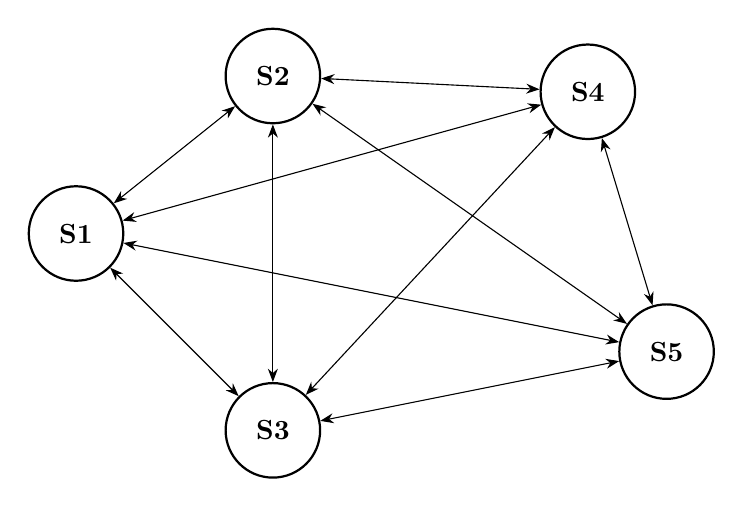
\begin{tikzpicture}[
        >=Stealth, % Arrowhead style
        site/.style={circle, draw, thick, minimum size=1.2cm, font=\bfseries}
    ]
    
    % ==========================================
    % Nodes Placement
    % ==========================================
    \node[site] (S1) at (0, 2) {S1};
    \node[site] (S2) at (2.5, 4) {S2};
    \node[site] (S4) at (6.5, 3.8) {S4};
    \node[site] (S5) at (7.5, 0.5) {S5};
    \node[site] (S3) at (2.5, -0.5) {S3};
    
    % ==========================================
    % Edges (Complete Graph Connections)
    % ==========================================
    
    % Connections from S1
    \draw[<->] (S1) -- (S2);
    \draw[<->] (S1) -- (S3);
    \draw[<->] (S1) -- (S4);
    \draw[<->] (S1) -- (S5);
    
    % Connections from S2
    \draw[<->] (S2) -- (S3);
    \draw[<->] (S2) -- (S4);
    \draw[<->] (S2) -- (S5);
    
    % Connections from S3
    \draw[<->] (S3) -- (S4);
    \draw[<->] (S3) -- (S5);
    
    % Connections from S4
    \draw[<->] (S4) -- (S5);

    \end{tikzpicture}
    
    \vspace{0.5cm}
    \textbf{Figure 1:} Distributed Database System consisting of five sites
    \vspace{0.5cm}

    \renewcommand{\arraystretch}{1.4} % Expands row height slightly for readability
    \begin{tabular}{|c|c|}
        \hline
        \textbf{T1} & \textbf{Data replication} \\
        \hline
        READ (A) & \multirow{5}{*}{%
            \begin{tabular}{c}
                Data item \textbf{A} is fragmented to S2, S4 \\[1em] 
                Data item \textbf{B} is fragmented to S2, S3, S5
            \end{tabular}%
        } \\
        \cline{1-1}
        READ (B) & \\
        \cline{1-1}
        WRITE (A) & \\
        \cline{1-1}
        WRITE (B) & \\
        \cline{1-1}
        COMMIT & \\
        \hline
    \end{tabular}
    
    \vspace{0.4cm}
    \textbf{Figure 2:} A transaction T1 initiated from S1 of Figure 1.

  \end{center}

\mk{20} \yr{CSE 303 | L-3/T-1 | 2015--16}

\end{enumerate}

%%──────────────────────────────────────────────────────────────────────
\subtopic{cE}{Big Data \& XML}
\label{sub:s8-bigdata}

\begin{enumerate}

%% Q1 — 2017-18 XML DTD
\item From the following Document Type Definition (DTD), describe the structure of the data in XML and write a sample XML file using this DTD:
\begin{lstlisting}[language=XML,morekeywords={DOCTYPE,ELEMENT,PCDATA}]
<!DOCTYPE STARS [
  <!ELEMENT STARS (STAR*)>
  <!ELEMENT STAR (NAME, ADDRESS+, MOVIES)>
  <!ELEMENT NAME (#PCDATA)>
  <!ELEMENT ADDRESS (STREET, CITY)>
  <!ELEMENT STREET (#PCDATA)>
  <!ELEMENT CITY (#PCDATA)>
  <!ELEMENT MOVIES (MOVIE*)>
  <!ELEMENT MOVIE (TITLE, YEAR)>
  <!ELEMENT TITLE (#PCDATA)>
  <!ELEMENT YEAR (#PCDATA)>
]>
\end{lstlisting}
\mk{10} \yr{CSE 215 | L-2/T-2 | 2017--18}

%% Q2 — 2017-18 MapReduce framework
\item Briefly describe the Map-Reduce framework.
\mk{5} \yr{CSE 215 | L-2/T-2 | 2017--18}

\end{enumerate}

%%──────────────────────────────────────────────────────────────────────
\subtopic{cE}{Table Partitioning}
\label{sub:s8-partition}

\begin{enumerate}

%% Q1 — 2021-22 table partitioning on Course Registration
\item Suppose BIIS has a large number of records in its Course Registration table, accumulated over the last 20 years. Explain how table partitioning can be done on this table, and what benefits and drawbacks it could offer.
\mk{10} \yr{CSE 215 | L-2/T-2 | 2021--22}

\end{enumerate}
\end{document}